\documentclass[11pt, a4paper, oneside]{book}
\usepackage[english]{babel}
\usepackage[utf8]{inputenc}
\usepackage[T1]{fontenc}
%\usepackage[subfigure]{tocloft}
\usepackage{graphics}
\usepackage[usenames,dvipsnames]{color}
\usepackage{graphicx} 
\usepackage{dcolumn}
\usepackage{bm}
\usepackage{epsfig}
\usepackage{pdflscape}
\usepackage{multirow}
\usepackage{rotating}
\usepackage{longtable}
\usepackage{lineno}
\usepackage[margin=1in,includefoot]{geometry}
\usepackage{fancyhdr}
\usepackage[hyphens]{url}
\usepackage{subcaption}
\usepackage{booktabs}
\usepackage{titlesec}
\usepackage[backend=bibtex]{biblatex}
\usepackage{float}
\usepackage{textcomp}
\usepackage[titletoc]{appendix}

\usepackage{titlesec, blindtext, color}
\definecolor{gray75}{gray}{0.75}
\newcommand{\hsp}{\hspace{20pt}}
\titleformat{\chapter}[hang]{\huge\bfseries}{\thechapter\hsp\textcolor{gray75}{|}\hsp}{0pt}{\huge\bfseries}

\addbibresource{references.bib}

%
%\titleformat{\chapter}[display]
%    {\normalfont\huge\bfseries}{\chaptertitlename\ \thechapter}{20pt}{\Huge}
\titlespacing*{\chapter}{0pt}{-20pt}{20pt} 

\usepackage{sidecap}
\usepackage{wrapfig}
\usepackage[separate-uncertainty = true,multi-part-units=single,detect-weight=true, detect-family=true]{siunitx}
\setlength\parindent{0pt} % No indent
\usepackage{physics}
\usepackage{enumitem}
\usepackage{ulem} % Adds \uline (nicer underline)
\usepackage{mhchem} % For element symbols
\usepackage{multirow} % Have rows spanning multiple columns in tables
\usepackage{pdfpages} % Include pdf in document
\usepackage{amsmath} % Center equations for example with \begin{gather}
\usepackage{amsthm} % Theorems, examples
\theoremstyle{definition} % Non-italic definitions
\usepackage{amssymb} % Adds symbols, e.g. \varnothing
\usepackage{amsfonts} % Natural/real numbers etc
\renewcommand{\labelenumi}{\roman{enumi}.} % Enumerate uses roman numerals
\usepackage{mathtools}
\usepackage{centernot} % Cross symbols, e.g. for does not imply
\usepackage{gensymb} % Adds \degree command
\usepackage{bbm} % Adds bbm fonts with \mathbbm{}
\usepackage{mathrsfs} % Adds e.g. \mathcal (fancy F)
\usepackage[many]{tcolorbox} % Colored boxes around equations
\usepackage{empheq}
\usepackage{microtype}

\newcommand{\Lim}[1]{\raisebox{0.5ex}{\scalebox{0.8}{$\displaystyle \lim_{#1}\;$}}} % Inline lim
\newcommand\myeq{\mathrel{\overset{\makebox[0pt]{\mbox{\tiny H.}}}{=}}} % Equals sign with H. above it

\newcommand{\R}{\mathbb{R}}
\newcommand{\C}{\mathbb{C}}
\newcommand{\Z}{\mathbb{Z}}
\newcommand{\N}{\mathbb{N}}
\newcommand{\Q}{\mathbb{Q}}

%\newcommand{\mathbf}{\vb*}

\pagestyle{fancy}

\renewcommand{\sectionmark}[1]{\markright{\S\;\arabic{section}.\ #1}}
%\renewcommand{\thechapter}{\Roman{chapter}}


\rhead{\nouppercase{\rightmark}}
\lhead{\nouppercase{\leftmark}}
\newcommand*{\rom}[1]{\expandafter\@slowromancap\romannumeral #1@}
\usepackage[colorlinks=true,linkcolor=blue]{hyperref}

\DeclareMathOperator{\arcsinh}{arcsinh}
\DeclareMathOperator{\supp}{supp}
\DeclareMathOperator{\gram}{gram}
\DeclareMathOperator{\rot}{rot}
\DeclareMathOperator{\divt}{div}
\DeclareMathOperator{\sgn}{sgn}

\hypersetup{
  colorlinks,
  citecolor=black,
  linkcolor=blue,
  urlcolor=Blue}
 

\begin{document}
%\begin{titlepage}
%
%\newcommand{\HRule}{\rule{0.88\linewidth}{0.3mm}}
%\newcommand{\HRulebeta}{\rule{\linewidth}{0mm}} % Defines a new command for the horizontal lines, change thickness here
%
%\center % Center everything on the page
% 
%%----------------------------------------------------------------------------------------
%%	HEADING SECTIONS
%%----------------------------------------------------------------------------------------
%\HRulebeta\\[0.5cm]
%
%
%\textsc{\LARGE Universität Zürich}\\[0.6cm] % Name of your university/college
%%\includegraphics[width=5cm]{Figures/universitas_turicensis.png}\\[1cm] % Include a department/university logo - this will require the graphicx package
%%\textsc{\Large Physics Lab Report
%%}\\[0.5cm] % Major heading such as course name
%%\textsc{\large Lab Report}\\[0.5cm] % Minor heading such as course title
%
%{\large Bachelorthesis}\\[0.8cm]
%%----------------------------------------------------------------------------------------
%%	TITLE SECTION
%%----------------------------------------------------------------------------------------
%
%\HRule \\[0.5cm]
%{\Large \bfseries Emergent Black Hole Dynamics in Critcal Floquet Systems} \\[0.2cm] % Title of your document
%\HRule \\[2cm]
%
% 
%%----------------------------------------------------------------------------------------
%%	AUTHOR SECTION
%%----------------------------------------------------------------------------------------
%
%\large Fabian Jaeger
%
%
%% If you don't want a supervisor, uncomment the two lines below and remove the section kukjgfop';ibcxvilywrq;ldpcm378flkmkrhello nathanhi,pdaskfiwhjcxkhdc0ldl,-rn;k3232jhdkas;jl'cf'ggdjjskald.   jjdnxksm.ao;df ja;ookallo. min name iscxh milahallo min name isch mila und du busch bl;d zzzzzzzzzzzzzzzz8                                                                  
%%\Large \emph{Author:}\\
%%John \textsc{Smith}\\[3cm] % Your name
%
%%----------------------------------------------------------------------------------------
%%	DATE SECTION
%%----------------------------------------------------------------------------------------
%
%%{\large October 17, 2017}\\[2cm] % Date, change the \today to a set date if you want to be precise
%
%\vfill % Fill the rest of the page with whitespace
%
%\end{titlepage}

\begin{titlepage}
    \centering
    \vspace*{0.5 cm}
    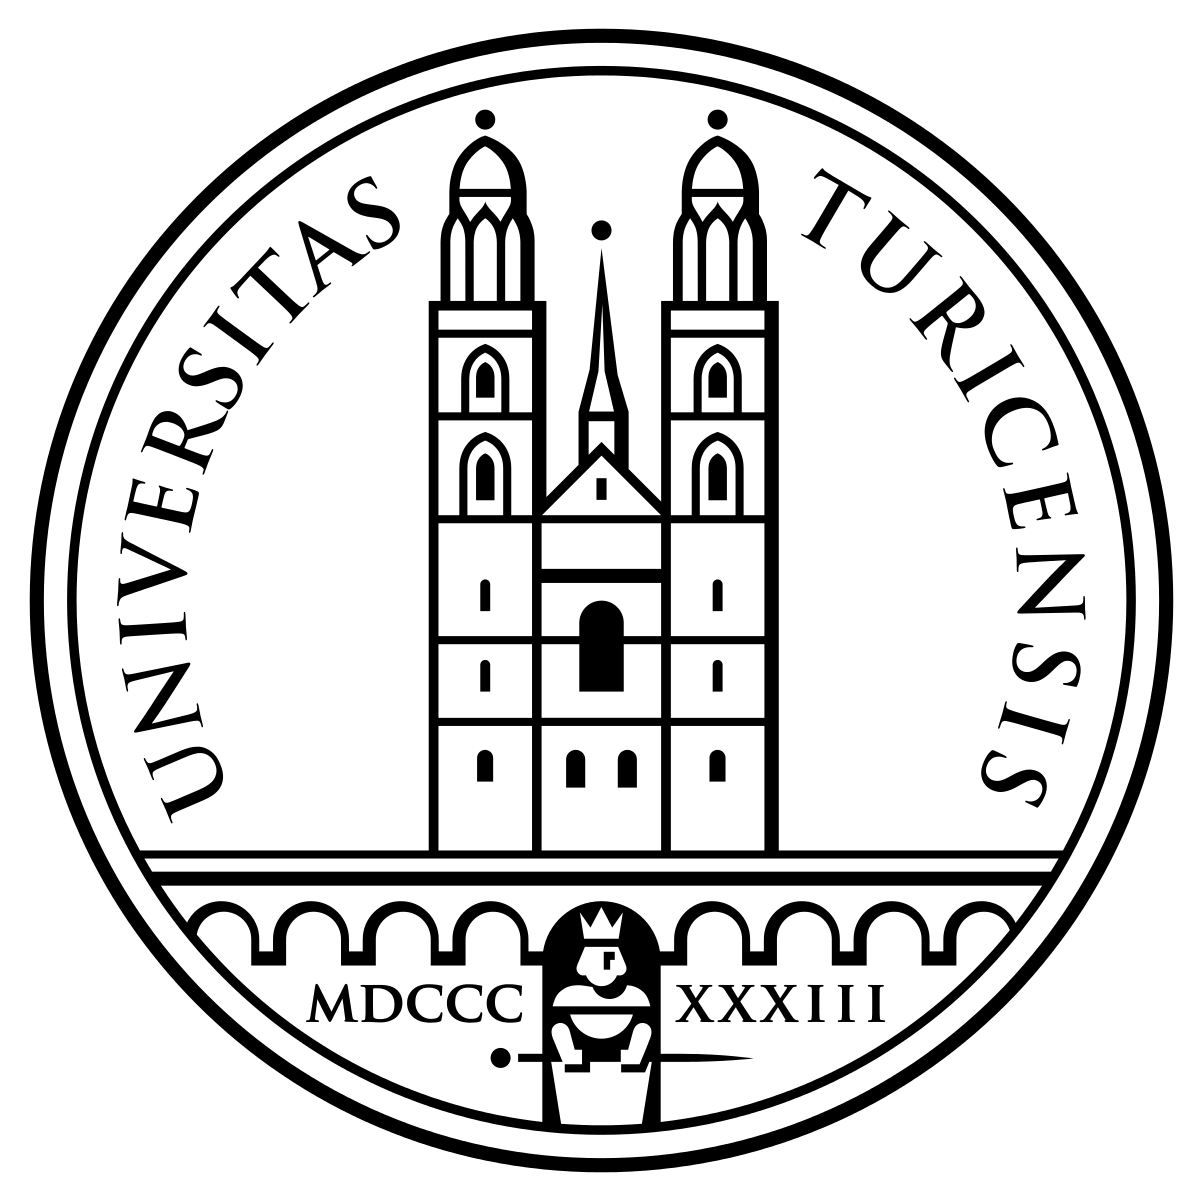
\includegraphics[width =0.34\textwidth]{UZH2.png}\\[1.2 cm]
      \textsc{\Large \textsc{Bachelorthesis}}\\[0.5 cm]

    \rule{\linewidth}{0.3 mm} \\[0.4cm]
    { \Large \bfseries Floquet dynamics of critical systems in one and higher dimensions}\\[0.3 cm]
    \rule{\linewidth}{0.3 mm} \\[1.5 cm]

  
    {\Large Fabian Jaeger}\\[2 cm] 
    
    
    		University of Zurich \\
             \textsc{Institute of Theoretical Physics} \\[1.5cm]
        
             	
    
    
    {\textbf{Supervised by}} \\[0.2cm]
   {\large  Prof. Dr. Titus Neupert} \\
   {\large Bastien Lapierre} \\ [2cm]
    
    {\large \today}\\[2 cm]
 
    \vfill
%    
%      \begin{minipage}{0.4\textwidth}
%        \begin{flushleft} \large
%            \textbf{Student}\\
%            \theauthor
%            \end{flushleft}
%            \end{minipage}~
%            \begin{minipage}{0.4\textwidth}
%            \begin{flushright} \large
%            \textbf{Enrollment Number} \\
%            17-740-325                                   % Your Student Number
%        \end{flushright}
%    \end{minipage}\\[1.2 cm]
    
\end{titlepage}


%\begin{abstract}
%    abstract-text
%\end{abstract}

\tableofcontents


\pagebreak
\hspace{0pt}
\vfill
\begin{center}\textbf{Acknowledgments}
\end{center}

I would like to sincerely thank Professor Titus Neupert for giving me this unique opportunity to work in his group. \\

I also want to express a great deal of gratitude towards my supervisor Bastien Lapierre for answering my questions, helping me in navigating through this difficult topic and generally being an invaluable mentor.\\

Finally, I wish to thank my family for their continued support.
\vfill
\hspace{0pt}
\pagebreak
%\chapter{Introduction}
%One intuition is based on the quasi-particle picture as presented in Sec.3.3. One can find that the existence of fixed point or not in the solution of equation of motion, which determines the system is in heating or non-heating phases, is independent of the introduction of finite temperature $\beta^{-1}$. We expect these two phases will persist even if the system is prepared at a thermal initial state. We leave the detailed study in a future work.
%The heating phase discussed here realizes a highly nonequlibrium state where entangled EPR pairs are continuously produced and localized at specific locations. Given the utility of entanglement as a resource for quantum information processing, experimental realization of the protocols discussed here may be desirable. Indeed given the high tunability of ultracold atomic systems in optical lattices [56], and the ability to measure both energy and entanglement entropy [57], an important future direction will be to find routes to implement these protocols in the lab.

% Write about the general field of Floquet Dyanmics

\chapter{Theory}
%This section serves as an introduction into the tight-binding model, effects of boundary conditions on the measurement of relevant quantities, the sine-square deformation and the Floquet system we will be considering for this thesis. Even though for our considerations, the explicit details of the tight-binding model will not be relevant for most of the thesis, a brief overview is still provided.

\section{Tight-binding model}
In solid-state theory, there are many models used to describe the interactions of electrons and their respective atoms on a lattice. In this thesis we will be considering the so-called tight-binding model, in which the electrons are, in contrast to the free-electron model, modeled to be closely bound to their respective atoms. For a theoretical model, this has the useful consequence, that the interaction of other atoms in the crystal lattice with those tightly bound electrons, can be regarded as negligible.  This tight-binding of the electrons motivates describing the electronic states as atomic orbital wave functions $\phi_A(\mathbf{r})$, rather than the commonly used plane waves $\exp(i \mathbf{k} \cdot \mathbf{r})$ in the free-electron model. Since the electrons are strongly localized to their respective atom, the atomic overlap of the atom wave functions of different atoms in the crystal lattice is therefore expected to be rather small \cite{Titus,Manfred}. \\

%The description of the tight-binding is therefore equivalent to stating the the resulting atomic overlap of the wave functions on different atoms is small
%
%and that the resulting atomic overlap of the wave functions on different atoms is small.
It should be noted that the tight-binding approximation is mainly employed for describing low-lying electron energy states (i.e $s$- or $p$-orbitals) due to their lower spatial extension. In this regime, the  atomic potential plays the vital role in determining the spectrum of our Hamiltonian and the atomic Hamiltonian for an isolated atom at position $\mathbf{R}$ is given by:
\begin{equation}
	\hat{H}_A(\mathbf{r} - \mathbf{R}) = -\frac{\hbar^2}{2m}\nabla^2 + V_A(\mathbf{r} - \mathbf{R})
	\label{eq:single_atomic_potential}
\end{equation}
where $\mathbf{r} - \mathbf{R}$ originates due to the dependence of the rotationally symmetric potential $V_A$ on the distance of the electron $\mathbf{r}$ of the position of the nucleus $\mathbf{R}$. The atomic Hamiltonian fulfills the following eigenvalue equation:
\begin{equation}
	\hat{H}_A \ket{i, \mathbf{R}} = E_A^i \ket{i, \mathbf{R}}
\end{equation}
where we denote $\ket{i, \mathbf{R}}$ to be the $i$-th energy state for the atom at lattice position $\mathbf{R}$ with the atomic orbital wave function:
\begin{equation}
	\braket{\mathbf{r}}{i, \mathbf{R}_j} = \psi_A^i(\mathbf{r} - \mathbf{R})
\end{equation}
Consequently, in the absence of any other atoms, the electrons bind with eigenstates $\psi_A^i(\mathbf{r} - \mathbf{R})$ and with energy $E_A^i < 0$ to the atom\footnote{In analogy to the potential, the eigenstates are functionally dependent on $\mathbf{r} - \mathbf{R}$}. \\

Our interest, however, lies in modeling a lattice of well separated atoms rather than a single isolated atom. To this end we extend our definition of the rotationally symmetric atomic potential $V_A$ to account for a lattice of atoms:
\begin{equation}
	V_\text{lattice}(\mathbf{r}) = \sum_{\mathbf{R}_i} V_A(\mathbf{r} - \mathbf{R}_i)
\end{equation}
 Extending our Hamiltonian to include the coulomb interaction of the electron at position $\mathbf{r}$ with the nucleus of atoms at all possible position $\mathbf{R}_i$ of the crystal lattice, we obtain:
\begin{equation}
	\hat{H} = - \frac{\hbar^2}{2m} \nabla^2 + \sum_{\mathbf{R}_j} V_A(\mathbf{r} - \mathbf{R}_j) = \hat{H}_A + \Delta V_{\mathbf{R}_j}
\end{equation}
where in the second step we split the single atomic potential (\ref{eq:single_atomic_potential}) from the correction term:
\begin{equation}
	\Delta V_{\mathbf{R}_j}(\mathbf{r}) = \sum_{\mathbf{R}_i \neq \mathbf{R}_j} V_A(\mathbf{r} - \mathbf{R}_i)
\end{equation}

Since the electrons at the different positions of the atoms are mostly localized (this refers to the electronic eigenfunctions $\psi_A^i(\mathbf{r})$ having a very small probability one lattice site away) and mainly interact with the closest atom, the correction term $\Delta V$ in the tight-binding approximation can be seen as a small perturbation of the atomic potential at position $\mathbf{R}_j$ due to the coulomb repulsion with the other atoms at the remaining sites $\mathbf{R}_i$, meaning close to each lattice point, the governing Hamiltonian is (\ref{eq:single_atomic_potential}) and, as already established, $\psi_A^i(\mathbf{r} - \mathbf{R})$ is a good approximation for low lying electronic energy state. This consequently motivates the use of a linear combination of atomic orbitals (LCAO):
\begin{equation}
	\psi_{i \mathbf{k}}(\mathbf{r}) = \frac{1}{\sqrt{N}} \sum_{\mathbf{R}_j} e^{i \mathbf{k} \cdot \mathbf{R}_j } \psi_{A}^i(\mathbf{r} - \mathbf{R}_j)
	\label{eq:LCAO_Ansatz}
\end{equation} 
where the normalized coefficient function in front of the atomic orbitals is obtained with the help of Bloch's theorem, stating that in a translationally symmetric system\footnote{Due to the fact that the Potential is assumed to be periodic, i.e $V(\mathbf{r} + a\mathbf{e}_i) = V(\mathbf{r})$}, the following holds:
\begin{equation}
	\psi_{i\mathbf{k}}(\mathbf{r} + \mathbf{R}_j) = e^{i \mathbf{k} \cdot \mathbf{R}_j} \psi_{i\mathbf{k}}(\mathbf{r})
\end{equation}

Electrons which are strongly bound to the atoms, i.e the ones with large binding energies, correspond to low lying energy states, which form the discrete spectrum shown in \ref{fig:illustration_tightbinding} will remain close to their host atoms. Those at higher energies, are more weakly bound and will be closer to free particles and have a chance to tunnel to neighboring atoms due to an overlap of the wave function with a neighboring atomic orbital. The weakly bound electrons which become dislodged from their host atoms are called valence electrons (the same electrons which typically sit in the outer shells) \cite{Singleton}\cite{Simon}\cite{Girvin}
\begin{figure}[h]
	\centering
	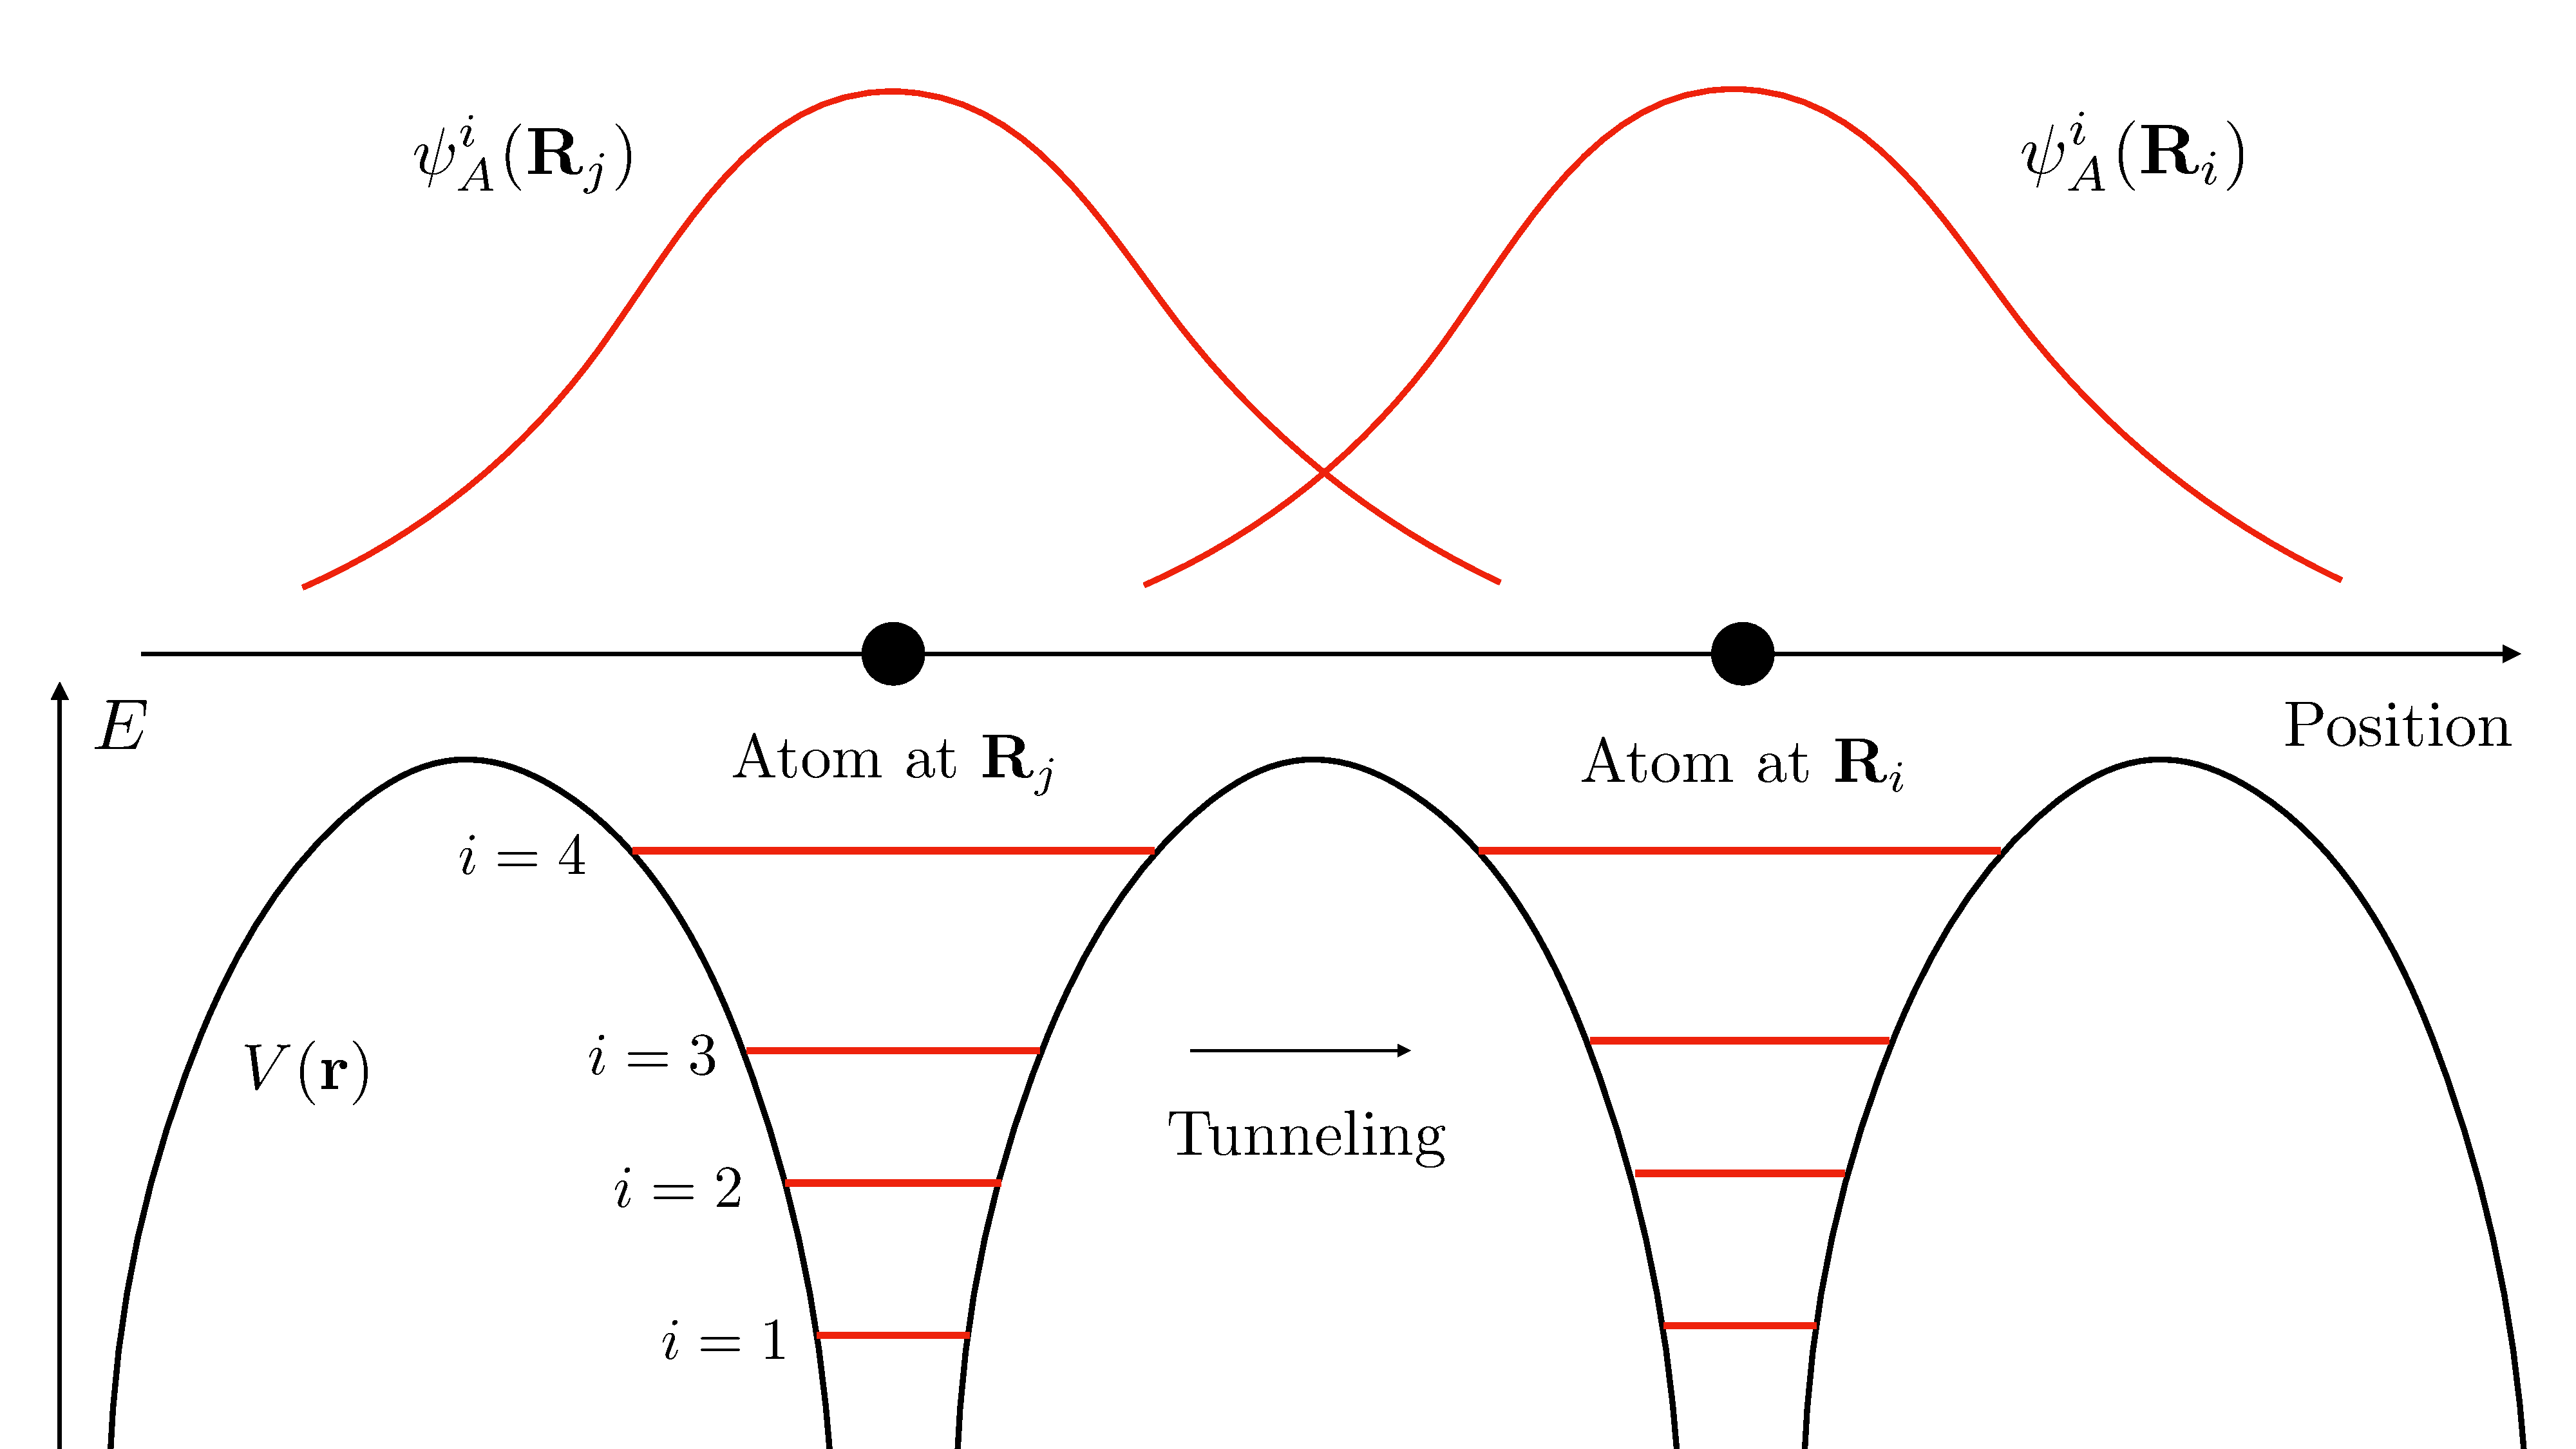
\includegraphics[width = 0.7\textwidth]{TightBindingModel-Illustration}
	\caption{Schematic illustration of the tight-binding model}
	\label{fig:illustration_tightbinding}
\end{figure}
Instead of labelling our energy states with the index $i$ we will use a generalized quantum number denoted by lowercase greek letters, $\alpha, \beta, \dots$ to include all other possible quantum numbers that uniquely determine an atomic orbital eigenstate (in the case of a hydrogen atom we would for example have $\alpha = (n_1,l_1,s_1)$). In Dirac notation, the LCAO ansatz (\ref{eq:LCAO_Ansatz}) then takes the form:
\begin{equation}
	\ket{\psi_{\alpha\mathbf{k}}} = \frac{1}{\sqrt{N}} \sum_{j=1}^N e^{i \mathbf{k} \cdot \mathbf{R}_j} \ket{\alpha, \mathbf{R}_j}
	\label{eq:LCAO_ansatz}
\end{equation}
Since the pre-factor is simply a phase, computing the matrix elements of the Hamiltonian with $\ket{\psi_{\alpha \mathbf{k}}}$ boils down to finding the explicit matrix form of: 
%\begin{equation}
%	\mel{\alpha, \mathbf{R}_j}{\hat{H}}{\beta, \mathbf{R}_i} = \mel{\alpha, \mathbf{R}_j}{\hat{H}_A}{\beta, \mathbf{R}_i} + \mel{\alpha,\mathbf{R}_j}{\Delta \hat{V}_{\mathbf{R}_j}}{\beta, \mathbf{R}_i}
%\end{equation}
\begin{equation}
	\mel{\alpha, \mathbf{R}_j}{\hat{H}}{\beta, \mathbf{R}_i} = E_{\alpha} \delta_{\alpha,\beta} \delta_{\mathbf{R}_j, \mathbf{R}_i} + \mel{\alpha,\mathbf{R}_j}{\Delta \hat{V}_{\mathbf{R}_j}}{\beta, \mathbf{R}_i}
\end{equation}
In further considerations of the tight-binding model we will consider a single orbital for each atom on the lattice (for example the $s$-orbital) and neglect the irrelevant global diagonal energy shift resulting from the first term. If we consider a trivially spin-degenerate system, we can drop the index $\alpha$ and aim to focus entirely on the overlap integral or hopping matrix elements $\mel{\mathbf{R}_j}{\Delta V_{\mathbf{R}_j}}{\mathbf{R}_i}$ \cite{Manfred, Titus}.

%It should be noted that the LCAO approach is variational in its nature, meaning that by increasing the size of the Hilbert space we only improve the accuracy of our model. However a resulting complication is that 
%
%
%
%It should be noted that the solutions are not exakt but rather obtained using a variational approach. By increasing the amount of orbitals and therefore the Hilbert space we can improve the accuracy of the model. If we include more than one orbital per atom, i.e we do not simply have $\ket{\alpha,\mathbf{R}_j}$ but rather a set of $\alpha$'s per atomic site, the assumed orthogonality relation:
%\begin{equation}
%	\braket{\alpha, \mathbf{R}_j}{\beta, \mathbf{R}_j} = \delta_{\alpha\beta} \delta_{\mathbf{R}_j\mathbf{R}_i}
%\end{equation}
%The expected energy for the LCAO state is then the variational Ansatz \cite{Manfred}
 

%% Needs to be rewritten, mostly copied from book Girvin
%If we restrict our attention to this single orbital on each atom, then Bloch's theorem uniquely constrains the form of the eigenfunction in a Bravais lattice with lattice vector $\mathbf{k}$ to be
%\begin{equation}
%	\ket{\psi_{\mathbf{k}}} = \frac{1}{\sqrt{N}} \sum_{j=1}^N e^{i \mathbf{q} \cdot \mathbf{R}_j} \ket{\alpha, \mathbf{R}_j}
%\end{equation}
%To see why this is, consider
%\begin{align}
%	\braket{\mathbf{r}}{\psi_{\mathbf{k}}} &= \psi_{\mathbf{k}}(\mathbf{r}) = \frac{1}{\sqrt{N}} \sum_j e^{i \mathbf{k} \cdot \mathbf{R}_j} \phi_A^{\alpha}(\mathbf{r} - \mathbf{R}_j) \\
%	&= e^{i \mathbf{k} \cdot \mathbf{r}} u_{\mathbf{k}}(\mathbf{r})
%\end{align}
%with
%\begin{equation}
%	u_{\mathbf{k}}(\mathbf{r}) = \frac{1}{\sqrt{N}} \sum_{j=1}^N e^{-i\mathbf{k} \cdot (\mathbf{r} - \mathbf{R}_j)} \phi_A^\alpha(\mathbf{r} - \mathbf{R}_j)
%\end{equation}
%We can check that the same periodicity of the potential $V(\mathbf{r} + \mathbf{a}) = V(\mathbf{r})$ holds for the function $u_{\mathbf{k}}(\mathbf{r} + \mathbf{a}) = u_{\mathbf{k}}(\mathbf{r})$
%\begin{equation}
%	u_k(\mathbf{r} + \mathbf{a}) = \frac{1}{\sqrt{N}} \sum_{j=1}^N e^{i \mathbf{k} \cdot (\mathbf{r} + \mathbf{a} - \mathbf{R}_j)} \phi(\mathbf{r} + \mathbf{a} - \mathbf{R}_j) = \frac{1}{\sqrt{N}} \sum_{i=1}^N e^{i \mathbf{k} \cdot (\mathbf{r} - \mathbf{R}_{i})} \phi_{A}^\alpha(\mathbf{r} - \mathbf{R}_i)
%\end{equation}
%which is equivalent to stating that $\psi_{\mathbf{k}}(\mathbf{k} + \mathbf{a}) =e^{i \mathbf{k} \cdot \mathbf{a}} \psi_{\mathbf{k}}(\mathbf{x})$.




%\begin{equation}
%	E(\mathbf{k}) = \frac{\mel{\psi_{n\
%\end{equation}
%\subsection{Solution to tight-binding model in 1D}
%To obtain our energy expectation values
%
%\begin{equation}
%	\mel{\alpha, \mathbf{R}_j}{\hat{H}}{\beta, \mathbf{R}_i} =  \epsilon_0 + \Lambda(\mathbf{k})
%\end{equation}
%
%
%which means for the matrix elements we consider
%\begin{equation}
%	H_{n,m} = \epsilon_0 \delta_{n,m} - t(\delta_{n+1, m} + \delta_{n-1},m)
%\end{equation}
%
%%\begin{equation}
%%	\mel{\alpha, \mathbf{R}_j}{\Delta V_{\mathbf{R}_j}}{\beta, \mathbf{R}_i} = \begin{cases}
%%		V_0 \quad 
%%	\end{cases}
%%\end{equation}


\subsection{Tight-binding model in second quantized formalism}
Instead of working in first quantized form, it is beneficial to instead work in second quantization form. In second quantization the state of the lattice is expressed in terms of the occupation number of electrons at a given site. For a lattice with $N$ sites labeled by the lattice vectors $\mathbf{R}_j$ with $j = 1, \dots N$ we have the occupation number representation $\ket{n_1, \dots n_N}$. We define  the fermionic creation- $\hat{c}^\dagger_{\mathbf{R}_j}$ and annihilation $\hat{c}_{\mathbf{R}_j}$ operators in position space which create or annihilate a particle in the $j$-th site in a given orbital (we again assume we have a single orbital), which satisfy the fermionic anti-commutation relations
\begin{equation}
	\{\hat{c}_{\mathbf{R}_j}, \hat{c}_{\mathbf{R}_i}^\dagger\} = \delta_{ij} \qq{and} \{\hat{c}_{\mathbf{R}_j}, \hat{c}_{\mathbf{R}_i}\} = \{\hat{c}_{\mathbf{R}_j}^\dagger, \hat{c}_{\mathbf{R}_i}^\dagger\} = 0
	\label{eq:anti_commutation_relations_fermions}
\end{equation}
We note that the electron state depends mostly on the Fourier pre-factor
\begin{equation}
	\phi_j = \frac{1}{\sqrt{N}} e^{i \mathbf{k} \cdot \mathbf{R}_j}
\end{equation}
rather than the explicit form of the orbital, which means our study will mainly involve $\phi_j$. It should however always remembered that the exact electron state is given by the product of $\phi_j$ with the orbital at the position $\mathbf{R}_j$.
In position space, the tight-binding Hamiltonian in second quantization is then given by:
\begin{equation}
	\hat{H}_\text{tight-binding} = \sum_{j} E_0 \hat{c}_{\mathbf{R}_j}^\dagger \hat{c}_{\mathbf{R}_j} + \sum_{\mathbf{R}_i, \mathbf{R}_j} t_{ij} \hat{c}_{\mathbf{R}_i}^\dagger \hat{c}_{\mathbf{R}_j} + \text{h.c}
	\label{eq:tight_binding_Hamiltonian}
\end{equation}
The 'h.c' in this case denotes the hermitian conjugate, i.e the adjoint operator. The matrix elements $t_{ij} = t_{ji}$ are referred to as hopping elements where $t_{ij}^2$ determines the probability that an electron on site $i$ hops to site $j$ and is of the dimension of energy. The hermitian conjugate then describes the inverse operation, i.e the annihilation of the electron at position $\mathbf{R}_i$ and subsequently a creation of the electron at site $\mathbf{R}_j$. Since the operator product $\hat{c}_i^\dagger \hat{c}_j$ annihilates an electron on site $\mathbf{R}_j$ and creates one on site $\mathbf{R}_i$, it represents the kinetic energy of the electron. Instead of considering all possible interactions with the potentials at all sites, we want to restrict ourselves to identical nearest neighbor interactions at every position $\mathbf{R}_j$, meaning we set:
\begin{equation}
	t_{ij} = \mel{\mathbf{R}_j}{\Delta \hat{V}_{\mathbf{R}_j}}{\mathbf{R}_l} = \begin{dcases}
		-t \quad &\text{if $\mathbf{R}_j$ and $\mathbf{R}_i$ are nearest neighbors }\\
		0 \quad & \text{otherwise}
		\end{dcases}
\end{equation}
and the Hamiltonian (\ref{eq:tight_binding_Hamiltonian}), without the irrelevant global energy shift, takes the following form:
\begin{equation}
	\hat{H}_{\text{tight-binding}} = - t \sum_{\expval{\mathbf{R}_j, \mathbf{R}_i}} \hat{c}_{\mathbf{R}_j}^\dagger \hat{c}_{\mathbf{R}_i} + \text{h.c} = -\frac{t}{2} \sum_{j}\sum_{\bm{\delta}} (\hat{c}_j^\dagger \hat{c}_{j + \bm{\delta}} + \hat{c}_{j + \bm{\delta}}^\dagger \hat{c}_j)
	\label{eq:general_tight_binding_secondquant}
\end{equation}
where in the second step we expanded the nearest neighbor sum $\expval{\mathbf{R}_j,\mathbf{R}_i}$ and included the factor 1/2 to avoid double counting. For a $d$-dimensional Bravais lattice without diagonal hoppings, $\sum_{\bm{\delta}}$ sums over all the $q = 2d$ unique nearest neighbor vectors $\bm{\delta}_1, \bm{\delta}_2, \dots \bm{\delta}_q$ for any lattice site $j$.

%\begin{equation}
%	t_{ij} = \mel{\mathbf{R}_j}{\Delta \hat{V}_{\text{atom, \mathbf{R}_j}}}{\mathbf{R}_l} = \begin{dcases}
%		-t \quad &if $\mathbf{R}_j$ and $\mathbf{R}_l$ are nearest neighbors \\
%		0 \quad &otherwise
%	\end{dcases}
%\end{equation}
%To emphasize, we generally would have to include the spin degrees of freedom but we simply consider a trivially spin degenerate system in this thesis.

\subsection{Momentum space representation}
\label{sec:monentum_space_representation}
Instead of labeling the state of the lattice with the positions of the electrons we can also express it with the number of electrons with a given momenta $\ket{\mathbf{k}}$. It should be noted, that $\hbar \mathbf{k}$ is not the electron moment but rather the crystal momentum, i.e the momentum of the system (for a discussion, see for example \cite{Singleton}, section 5.2.1). It's better to think of it as the quantum number which uniquely determines a Bloch state. For a second quantized operator, a change of basis corresponds to:
\begin{equation}
	\hat{c}_\alpha^\dagger = \sum_\beta \braket{\beta}{\alpha} \hat{c}_\beta^\dagger \qq{and} \hat{c}_\alpha = \sum_\beta \braket{\alpha}{\beta} \hat{c}_\beta
\end{equation}
where $\{\ket{\alpha} \}$ and $\{\ket{\beta}\}$ are a full set of orthonormal basis states that span the Hilbert space. The relevant element is the projection of the basis elements of one space onto the other, which in case of the Fourier space results in the following inner product between basis elements:
\begin{equation}
	\braket{\mathbf{k}}{j} = \psi_{\mathbf{k}}^*(\mathbf{R}_j) = \frac{1}{\sqrt{N}} e^{-i \mathbf{k} \cdot \mathbf{R}_j} \qq{and} \braket{j}{\mathbf{k}} = \psi_\mathbf{k}(\mathbf{R}_j) = \frac{1}{\sqrt{N}} e^{i \mathbf{k} \cdot \mathbf{R}_j}
\end{equation}
where $\ket{j} = \hat{c}_{\mathbf{R}_j}^\dagger \ket{0}$ is the state with an electron on the $j$-th site. Here $\ket{0}$ defines the vacuum state. The creation and annihilation operators in momentum space then have following representation:
\begin{equation}
	\hat{c}_{\mathbf{k}} = \frac{1}{\sqrt{N}}  \sum_{\mathbf{k}} e^{-i \mathbf{k}\cdot \mathbf{R}_j} \hat{c}_{\mathbf{R}_j} \qq{and} \hat{c}_\mathbf{k}^\dagger = \frac{1}{\sqrt{N}} \sum_\mathbf{k} e^{i \mathbf{k} \cdot \mathbf{R}_j} \hat{c}_{\mathbf{R}_j}^\dagger
\end{equation}
where the sum over momentums $\mathbf{k}$ is taken over the first brillouin zone. In 1D, this would mean, $\mathbf{k} = 2\pi n/ N$ with $n = 0, \dots, N$ where $L = Na$. The inverted expression then yields us:
\begin{equation}
	\hat{c}_{\mathbf{R}_j} = \frac{1}{\sqrt{N}} \sum_{\mathbf{k}} e^{i \mathbf{k}\cdot \mathbf{R}_j} \hat{c}_\mathbf{k} \qq{and} \hat{c}_{\mathbf{R}_j}^\dagger = \frac{1}{\sqrt{N}} \sum_{\mathbf{k}} e^{-i\mathbf{k}\cdot \mathbf{R}_j} \hat{c}_\mathbf{k}^\dagger
\end{equation}
Rewriting the Hamiltonian (\ref{eq:general_tight_binding_secondquant}) in terms our momentum space operators yields:
\begin{equation}
\begin{split}
	\hat{H}_{tb} &= - \frac{t}{2N} \sum_j \sum_{\bm{\delta}, \mathbf{k}, \mathbf{k}'} (e^{-i \mathbf{k} \cdot \mathbf{R}_j} e^{i \mathbf{k}' \cdot (\mathbf{R}_j + \bm{\delta})} \hat{c}^\dagger_{\mathbf{k}} \hat{c}_{\mathbf{k}'} + e^{-i \mathbf{k}' \cdot (\mathbf{R}_j + \bm{\delta})} e^{i \mathbf{k} \cdot \mathbf{R}_j} \hat{c}_{\mathbf{k}}^\dagger \hat{c}_{\mathbf{k}'} ) \\
	&= -\frac{t}{2} \sum_{\bm{\delta}, \mathbf{k}} (e^{i \mathbf{k} \cdot \bm{\delta}} +  e^{_-i\mathbf{k} \cdot \bm{\delta}}) \hat{c}_{\mathbf{k}}^\dagger \hat{c}_{\mathbf{k}} = - \frac{t}{2} \sum_{\bm{\delta}, \mathbf{k}} \cos(\mathbf{k} \cdot \bm{\delta}) \hat{c}_{\mathbf{k}}^\dagger\hat{c}_{\mathbf{k}}
\end{split}
\end{equation}
where we used the relation:
\begin{equation}
	\sum_{\mathbf{k}} e^{i(\mathbf{k} - \mathbf{k}')\mathbf{R}_j} = N \delta_{\mathbf{k},\mathbf{k}'}
\end{equation}
The diagonalized Hamiltonian in momentum space can then be written as:
\begin{equation}
	\hat{\mathcal{H}}_{\text{tight-binding}} = \sum_{\mathbf{k}} \epsilon_{\mathbf{k}} \hat{c}_{\mathbf{k}}^\dagger \hat{c}_{\mathbf{k}}
\end{equation}
with the dispersion relation
\begin{equation}
	\epsilon_{\mathbf{k}} = -t\sum_{\bm{\delta}} \cos(\mathbf{k} \cdot \bm{\delta})
	\label{eq:dispersion_relation}
\end{equation}
This allows us to directly see, that the eigenstates of $\hat{H}_{tb}$ are then uniquely defined by giving the occupation number $n_{\mathbf{k}} = \hat{c}_{\mathbf{k}}^\dagger \hat{c}_{\mathbf{k}} = \{0,1\}$ for every single particle state. The associated eigenvalue $E_a$ for an arbitrary state $\ket{A}$ is then given by $E_a = \sum_{\mathbf{k}} \epsilon_\mathbf{k}$ with the sum running over the state in $\ket{A}$ for which $n_{\mathbf{k}} = 1$. For a system with a fixed number of electrons $N_g$, the occupation number satisfy the constraint
\begin{equation}
	\sum_{\mathbf{k}} n_{\mathbf{k}} = N_g
\end{equation}
and the ground state $\ket{G}$ corresponds to the system in which the states with the smallest energies $\epsilon_{\mathbf{k}}$ are filled. The $k$-states that will be filled are the ones up to the Fermi wavevector $\mathbf{k}_F$. Thus we write the ground state generally as:
\begin{equation}
	\ket{G} = \prod_{\mathbf{k} < \mathbf{k}_F} \hat{c}_{\mathbf{k}}^\dagger \ket{0}
\end{equation}
where $\ket{0}$ denotes the vacuum state, i.e the state in which no electrons are present. The explicit form of the dispersion relations is obtained, once a proper lattice structure has been determined. In our thesis, we will consider both the one-dimensional chain and the two-dimensional square lattice at half filling.

\subsection{One dimensional chain}
For a simple one-dimensional chain, for each lattice site,  the nearest neighbor vectors are \cite{Utermohlen}
\begin{equation}
	\delta_1 = a, \qq{and} \delta_2 = -a
\end{equation}
with the lattice constant $a$, resulting in the following Hamiltonian in real space:
\begin{equation}
	\hat{H}_{\text{tight-binding}} = -\frac{t}{2}\sum_{j=1}^N(\hat{c}_j^\dagger \hat{c}_{j + a} + \hat{c}_{j + a}^\dagger \hat{c}_j)
\end{equation}
The energy dispersion relation is obtained by correctly inserting the nearest neighbors into equation (\ref{eq:dispersion_relation}):
\begin{equation}
	\epsilon_k = -t \left[ \cos(ka) + \cos(-ka)\right] = -2t\cos(ka)
\end{equation}
and the tight binding hamiltonian in momentum space for a single orbital is:
\begin{equation}
	\hat{\mathcal{H}}_{\text{tight-binding}} = -2t \sum_{k} \cos(ka) \hat{c}_{k}^\dagger \hat{c}_{k}
\end{equation}
Since, the dispersion relation is periodic in $k \rightarrow k + 2\pi/a$, we restrict ourselves to the first Brillouin zone. Similar to the phonon case, and unlike the free-particle model, the electrons have a minimum and maximum energy within a given band and a vanishing group velocity at the Brillouin zone boundary: $v_G  = \partial{E}/\partial{k}\eval_{k = k_F} = 0$. If $N \rightarrow \infty$, the wavevector $k$ has values from the first Brillouin zone, i.e in the range $[-\pi/a, \pi/a]$. The negative $k$ vectors correspond to electrons moving to the right, while positive $k$ vectors correspond to electrons moving to the left  \cite{Simon}\cite{Singleton}. The dispersion relation is seen plotted in Figure \ref{fig:dispersion_relation1D}.\\

For an even system size, the ground state $\ket{G}$ for the chain at half filling, corresponds to the state, in which all the first $N/2$ $k$-states are occupied:
\begin{equation}
	\ket{G} = \sum_{k = 1}^{N/2} \hat{c}_k^\dagger\ket{0}
\end{equation}
and the ground state energy is simply obtained by summing up all negative eigenvalues, which for the spinless fermion model with $n_k = \{1,0\}$, corresponds to summing up to $N/2$:
\begin{equation}
	E_0 = \sum_{k=1}^{N/2} \epsilon_{k}
\end{equation}
In our computations, we will simply set the lattice constant to be equal to $a=1$ and the tight-binding Hamiltonian takes the form:
\begin{equation}
	\hat{H}_{\text{tb}} = - \frac{t}{2} \sum_{j=1}^{L-1}[\hat{c}_j^\dagger \hat{c}_{j+1} + \hat{c}_{j + 1}^\dagger \hat{c}_j]
\end{equation}

\subsection{Two-dimensional square lattice}
	\begin{figure}
		\centering
		\begin{subfigure}[t]{0.49\textwidth}
		\centering
			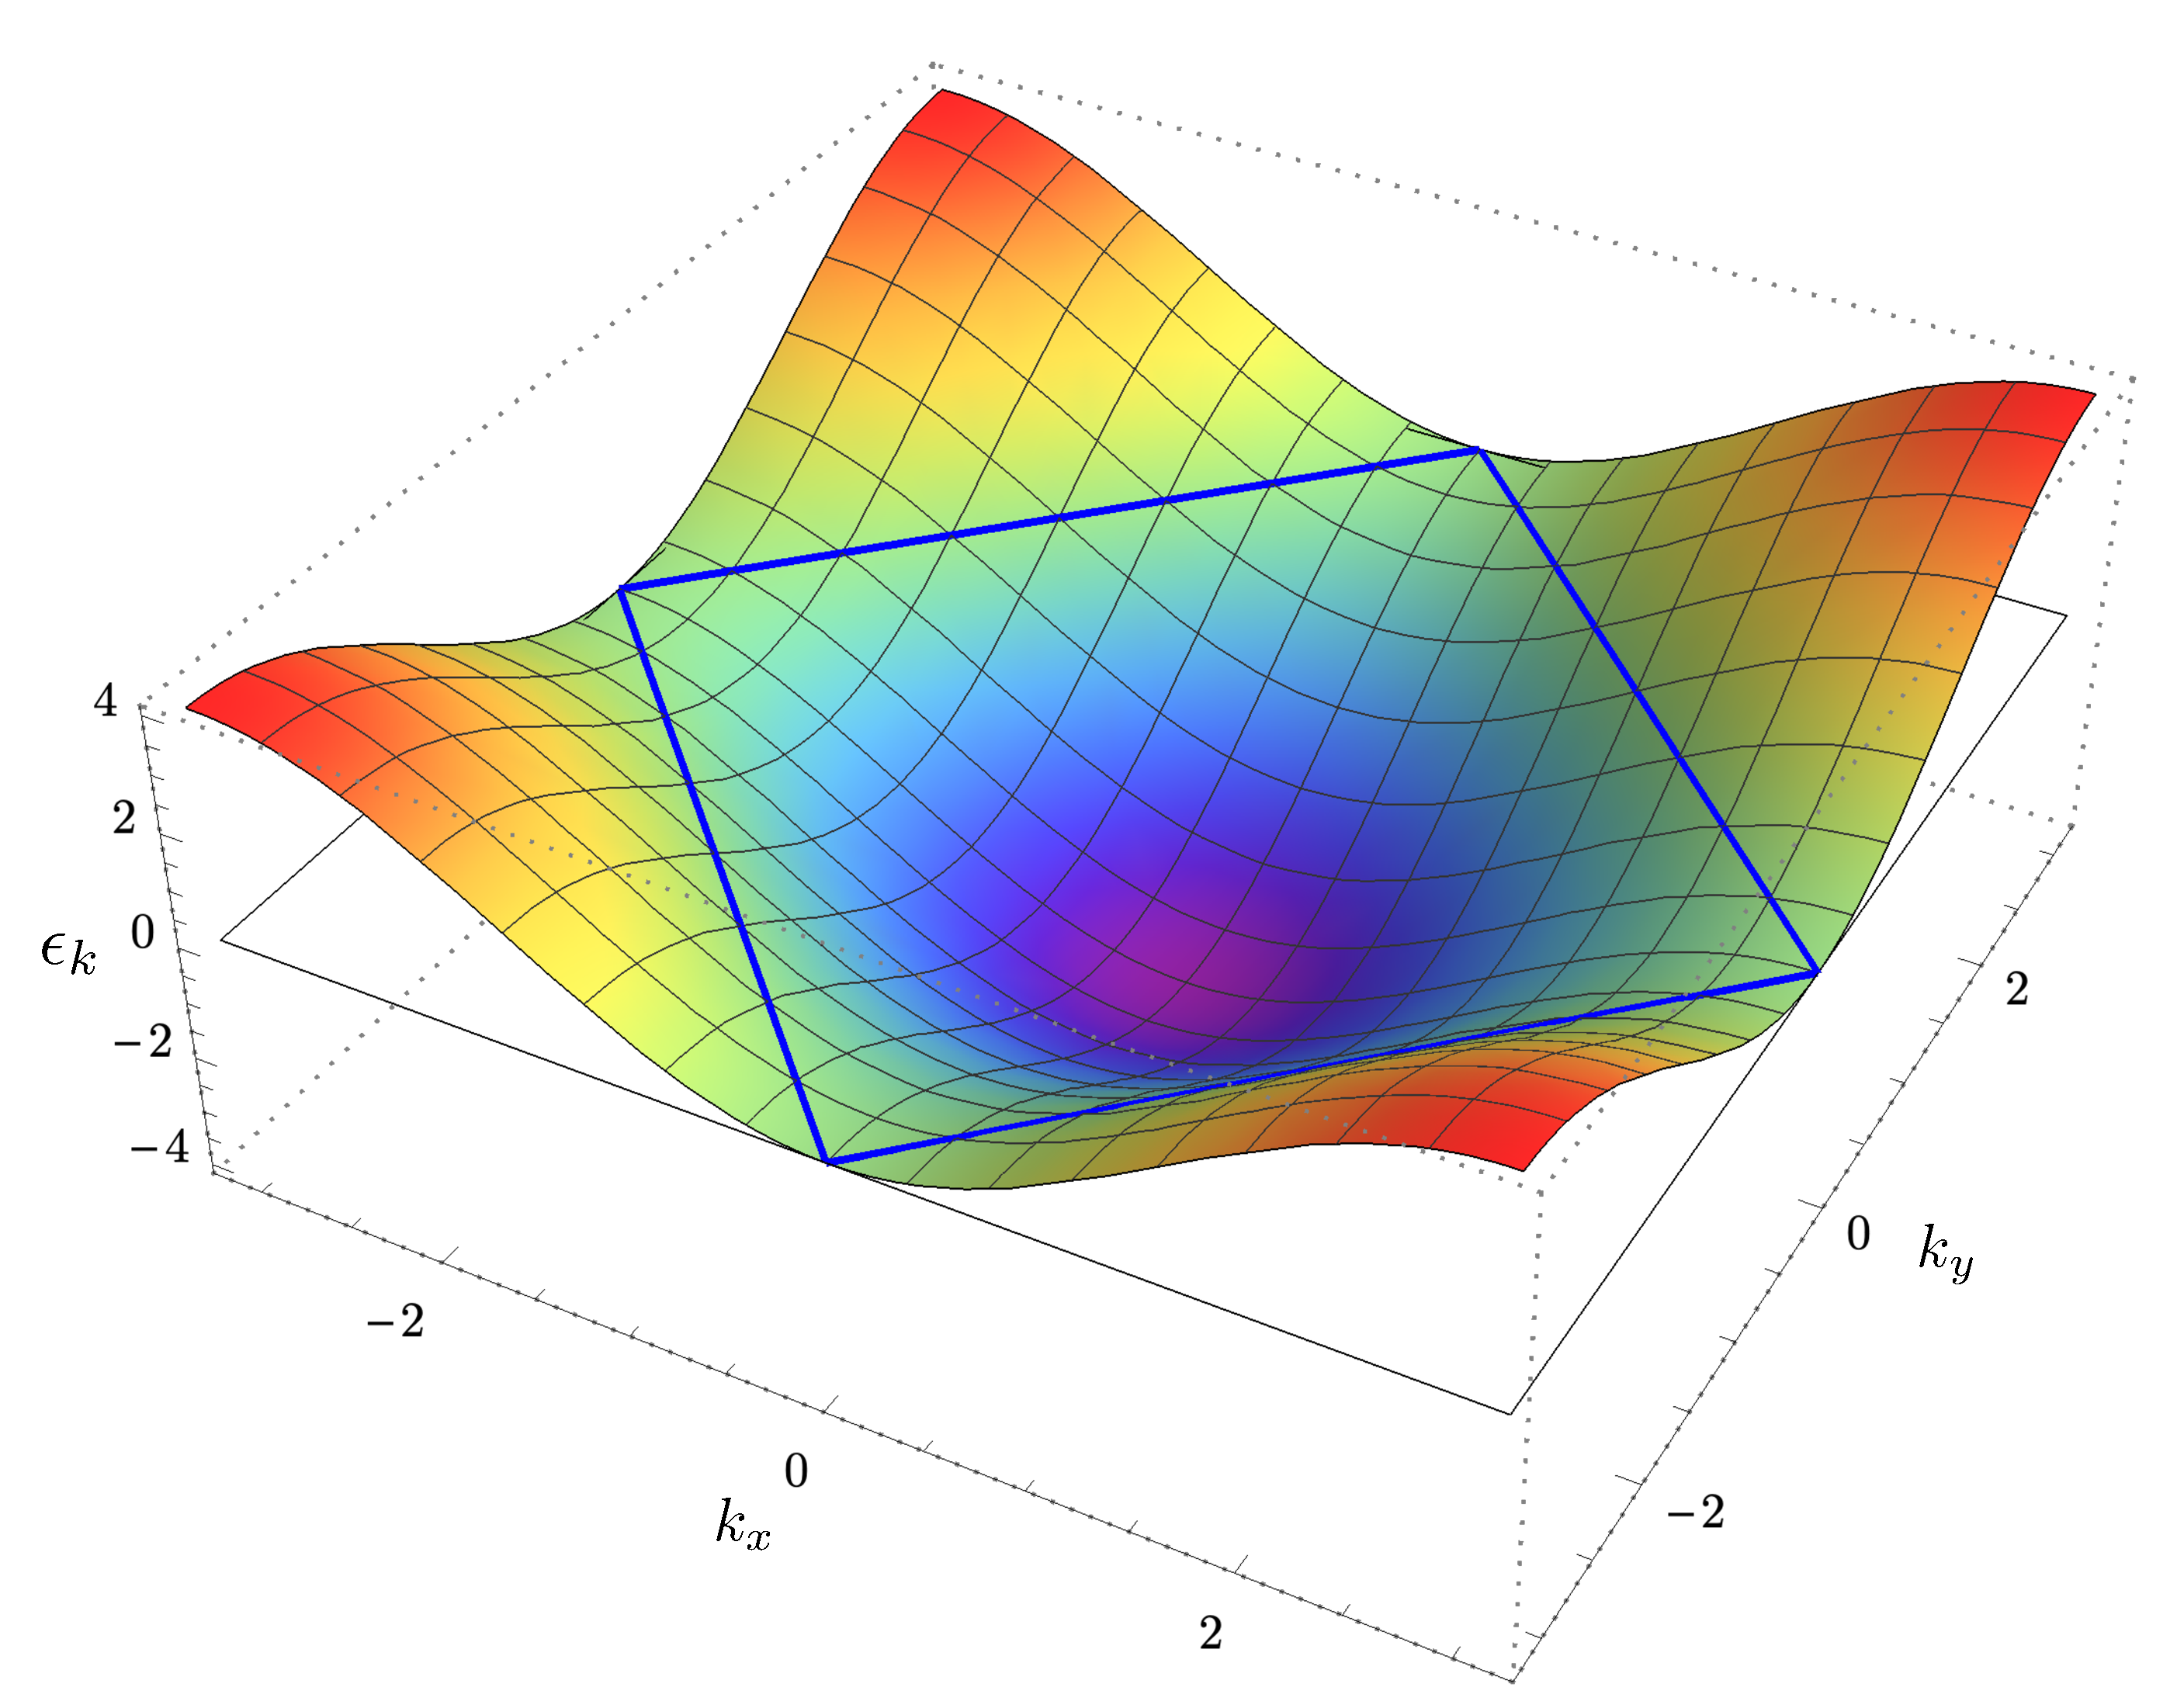
\includegraphics[width =\textwidth]{Dispersion_relation2d}
			\caption{}
		\end{subfigure}
		\begin{subfigure}[t]{0.49\textwidth}
		\centering
			\includegraphics[width =0.8\textwidth]{Dispersion_Relation2d_Top}
			\caption{}
		\end{subfigure}
		\caption{Dispersion Relation for a 2D tight binding Hamiltonian; (a) Dispersion relation for the tight binding Hamiltonian in two-dimensions for the first Brillouin zone. Up to the blue lines around the Energy $\epsilon_{\mathbf{k}} = 0$ the states are filled in the ground state. The Fermi surface separates the occupied states from the non-occupied ones.}
	\end{figure}
For a 2D square lattice, we have the following nearest neighbor vectors \cite{Utermohlen}:
\begin{equation}
	\bm{\delta}_1 = a \hat{\mathbf{x}}, \quad \bm{\delta}_2 = -a \hat{\mathbf{x}}, \quad \bm{\delta}_3 = a \hat{\mathbf{y}}, \quad \bm{\delta}_4 = -a \hat{\mathbf{y}}
\end{equation}
where again, $a$ represent the lattice constant, so the energy dispersion relation (\ref{eq:dispersion_relation})  is:
\begin{equation}
	\begin{split}
		\epsilon_{\mathbf{k}} &= -t \left[\cos(k_x a) + \cos(-k_x a) + \cos(k_y a) + \cos(-k_y a) \right] \\
		&= -2t\left[\cos(k_x a) + \cos(k_y a) \right]
	\end{split}
\end{equation}
and the tight-binding Hamiltonian in momentum space reads:
\begin{equation}
\begin{split}
	\hat{\mathcal{H}}_{\text{tb}} &= -2t\sum_{\mathbf{k}} (\cos(k_xa) + \cos(k_ya))\hat{c}^\dagger_{\mathbf{k}}\hat{c}_{\mathbf{k}}\\
	&= -2t\sum_{k_x, k_y} (\cos(k_xa) + \cos(k_ya))\hat{c}^\dagger(k_x, k_y)\hat{c}(k_x, k_y)
\end{split}
\end{equation}
If we again set the lattice constant in the square lattice model to be $a= 1$, the tight-binding model will take the form:
\begin{equation}
\begin{split}
\hat{H}_0 =  \sum_{i = 1}^{L_x-1} \sum_{j=1}^{L_y-1}& \Big( -\frac{t_1}{2} \left[ \hat{c}^\dagger(i, j) \hat{c}(i+1, j) + \hat{c}^\dagger(i+1, j)\hat{c}(i, j) \right] \\
	&-\frac{t_2}{2} \left[\hat{c}^\dagger(i,j) \hat{c}(i,j+1) + \hat{c}^\dagger(i, j+1)\hat{c}(i,j) \right] \Big) \\
\end{split}
\label{eq:tight_binding_2d_Hamiltonian}
\end{equation}


	

%
%Strictly speaking in a general tight-binding model we will additionally have to take into account the chemical potential $\mu$. For the one-dimensional lattice we therefore obtain
%\begin{equation}
%	\hat{H} = - t \sum_{j=1}^{L-1} \hat{c}_j^\dagger \hat{c}_{j+1} + \hat{c}_{j + 1}^\dagger \hat{c}_j - \mu \hat{c}_j^\dagger \hat{c}_j - \alpha t( \hat{c}_{L}^\dagger \hat{c}_1 + \hat{c}_1^\dagger \hat{c}_L)
%\end{equation}
%The parameter $\alpha$ serves to specify which boundary conditions we are using. For OBC we have $\alpha = 0$ and for PBC, $\alpha = 1$.  \\
%
%
%\begin{equation}
%\end{equation}
%The momentum-space representation of the tight-binding Hamiltonian is therefore
%\begin{equation}
%	\hat{H}_{tb} = \sum_{\mathbf{k}} \epsilon_{\mathbf{k}} \hat{c}_{\mathbf{k}}^\dagger \hat{c}_{\mathbf{k}}
%\end{equation}
%where
%\begin{equation}
%	\epsilon_{\mathbf{k}} = -t \sum_{\mathbf{\delta}} \cos(\mathbf{k} \cdot \mathbf{\delta})
%\end{equation}
%is the system's energy dispersion relation.
%\begin{equation}
%	\epsilon(l) = \begin{cases}
%		- 2t\cos(\frac{\pi l}{N+1}) &\qq{for OBC } (\alpha = 0) \\[10pt]
%		- 2t\cos(\frac{2\pi l}{N}) &\qq{for PBC } (\alpha = 1)
%	\end{cases}
%\end{equation}
%Often more compactly we write $\epsilon(k) = -2t\cos(ka)$ where the states with $k < 0$ represent electrons moving to the right and $k>0$ electrons moving to the left.
%

\section{Boundary conditions and sine-square Deformation}


%
%
%For any numerical study in this thesis our aim will be to obtain the properties of the system at the bulk and in the thermodynamic limit $N \rightarrow \infty$. In infinite systems, i.e in the thermodynamic limit, observables . Of interest will be to study how much the observables in the finite systems deviate from the ones in the thermodynamic limit, as those are ultimately the ones we wish to obtain. Finite size corrections can 


Observables for systems in the thermodynamic limit $N \rightarrow \infty$ are believed to be independent on the choice of boundary conditions. In this limit, we expect macroscopic thermodynamics to hold and all thermodynamic quantities to be only dependent on thermodynamic quantities, such as pressure and energy. However in numerical studies, which involve finite system sizes, the expectation values in the bulk of the system and the physical properties will crucially depend on the choice of boundary conditions. This is due to the fact that in finite systems, boundary conditions determine the topology of a system and the topology dictates the propagation of particles and information \cite{Hikihara}. Up until now, we often implicitly assumed periodic boundary conditions, to guarantee the analytical solvability of the model. Periodic boundary conditions are also employed, to suppress the boundary induced modulations resulting from open boundary conditions, which often present themselves as an obstacle in obtaining the expectation values in the bulk \cite{Hotta}\cite{Maruyama}\cite{Gendiar}. \\

  For the tight-binding model on a one-dimensional chain, the choice of boundary conditions, can then for example, be introduced with the variable $\alpha = \{1,0\}$:
\begin{equation}
	\hat{H} =  \sum_{j=1}^{L-1} \left[- \frac{t}{2} (\hat{c}_j^\dagger \hat{c}_{j+1} + \hat{c}_{j + 1}^\dagger \hat{c}_j)  - \mu\hat{c}_j^\dagger \hat{c}_j \right] - \alpha t( \hat{c}_{L}^\dagger \hat{c}_1 + \hat{c}_1^\dagger \hat{c}_L)
\end{equation}
where for completeness, the chemical potential $\mu$ is also included. Open boundary conditions, then correspond to $\alpha = 0$ and periodic boundary conditions to $\alpha = 1$, which we will from now on abbreviate with OBC and PBC, respectively. Topologically this means, that periodic boundary conditions, transform the system from a chain or cylinder to a ring or torus. The effects of the boundary conditions on the expectation value of an observable can for example be seen by considering the particle density $\expval{n_j} = \mel{G}{\hat{c}_j^\dagger \hat{c}_j}{G}$ in the ground state of the one-dimensional tight binding model at half-filling. For both OBC and PBC the relation:
\begin{equation}
	N_g = \sum_{i=1}^L \expval{n_j}
\end{equation}
always holds. However, for a translationally invariant system such as for PBC, the particle density is furthermore, as evident in Figure \ref{occupation_numer1_PBC}, a spatially uniform quantity corresponding to $N_g/L$. Additionally, as expected for open boundary conditions, in Figure \ref{fig:occupation_number1_OBC} we observe prominent oscillations around the open edges of the system \cite{Hotta}. \\
\begin{figure}[h]
\centering
\begin{subfigure}[t]{0.49\textwidth}
	\centering
	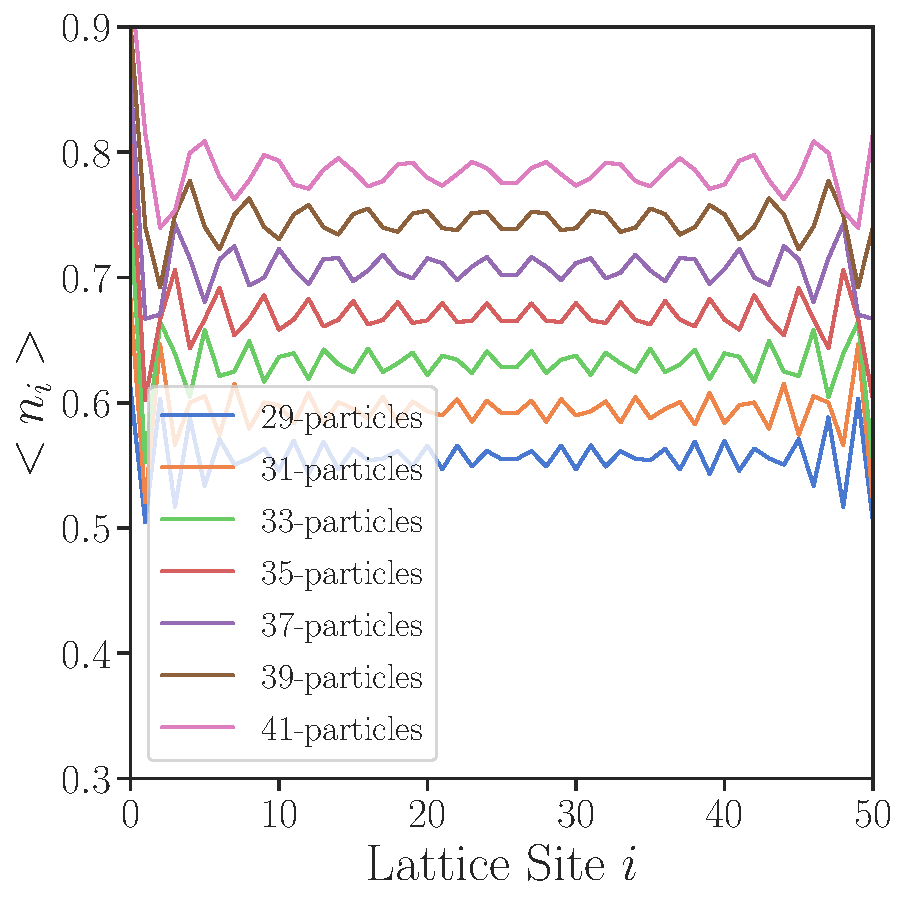
\includegraphics[width =\textwidth]{Occupation_number_H0_OBC}
	\caption{}
	\label{fig:occupation_number1_OBC}
\end{subfigure}
\begin{subfigure}[t]{0.49\textwidth}
	\centering
	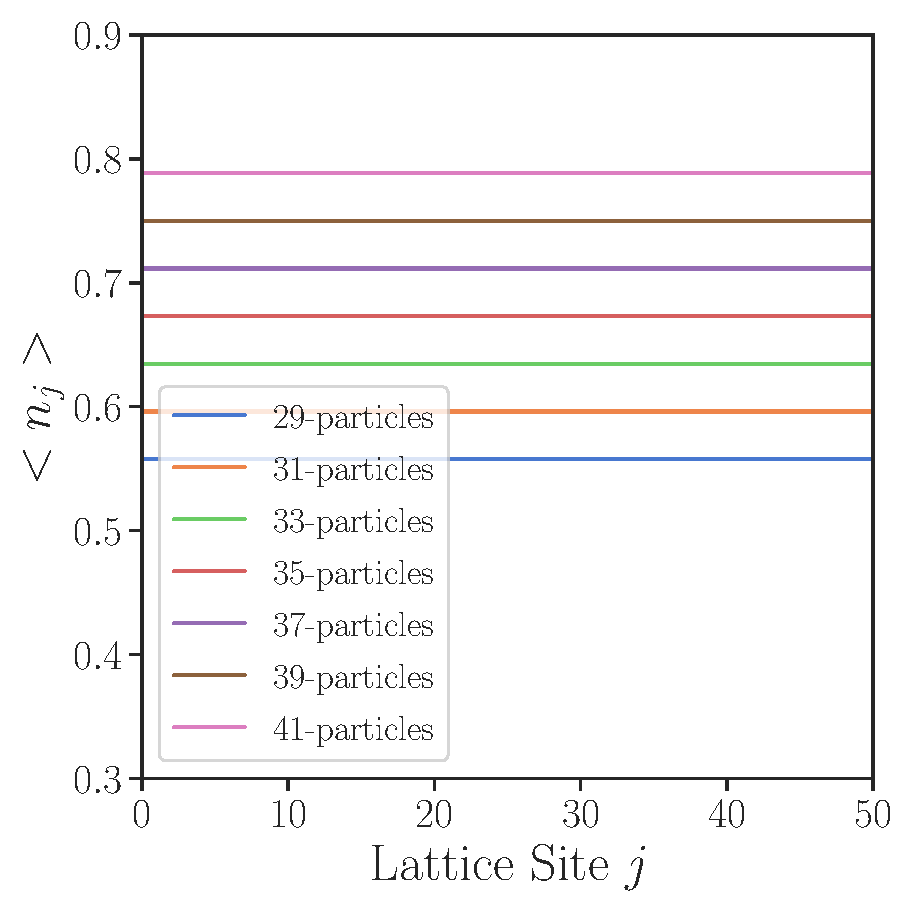
\includegraphics[width =\textwidth]{Occupation_number_H0_PBC}
	\caption{}
	\label{occupation_numer1_PBC}
\end{subfigure}
\caption{Occupation number $\expval{n_j}$ with different total particle numbers $N_g$ for (a) open-boundary conditions (b) periodic boundary conditions.}
\label{fig:occupation_number1d}
\end{figure}

In addition to periodic boundary conditions, so-called smooth boundary conditions can be employed, to efficiently suppress unwanted boundary effects and finite size errors resulting from open boundary conditions \cite{Hikihara}. Such models, are employed, when an open system is favored such as in the density matrix renormalization group or because it allows a Floquet system to be analytically solvable. One such model is the so called sine-squared deformation where an arbitrary Hamiltonian is locally rescaled according to the function \cite{Katsura2}:
\begin{equation}
	f_x = \sin^2\left[\frac{\pi}{L} \left(x -\frac{1}{2} \right)\right]
	\label{eq:scaling_function_SSD}
\end{equation}
Here $x$ denotes the local position and $L$ the length of the system. Unlike the case with PBC, the system with the sine-squared Hamiltonian is not translationally invariant, since it breaks the link between the sites $x=1$ and $x=L$. To construct the explicit form of the sine-squared deformed Hamiltonian for a one-dimensional chain of length $L$, we introduce the chiral deformation \cite{Maruyama, Katsura2}:
\begin{equation}
	\hat{H}^{(\pm)} = - \frac{t}{2} \sum_{j=1}^L e^{\pm i \delta x} [\hat{c}_j^\dagger \hat{c}_{j+1} + \text{h.c}] - \mu \sum_{j=1}^L e^{\pm i \delta(x - 1/2)} \hat{c}^\dagger_j \hat{c}_j
\end{equation}
where $\delta = 2\pi/L$. Each term in the sum of the chiral Hamiltonian is the discrete Fourier transformation of the local Hamiltonian. The sine-squared deformed tight-binding Hamiltonian can then be constructed as follows:
\begin{equation}
	\hat{H}_{\text{SSD}} = \frac{1}{2} \hat{H}_0 - \frac{1}{4} \left[\hat{H}^{(+)} + \hat{H}^{(-)}\right] = -\frac{t}{2} \sum_{j=1}^{L-1} f\left(j + \frac{1}{2}\right)[\hat{c}^\dagger_j \hat{c}_{j+1} + \text{h.c}] - \mu \sum_{j=1}^L f(j) \hat{c}_j^\dagger \hat{c}_j
	\label{eq:SSD_Hamiltonian_chiral}
\end{equation}
where $f(j)$ corresponds to the scaling function defined in equation (\ref{eq:scaling_function_SSD}). \\

\begin{figure}[h]
\centering
\begin{subfigure}[t]{0.49\textwidth}
	\centering
	\includegraphics[width =\textwidth]{BondEnergy2}
	\caption{}
	\label{BondEnergy}
\end{subfigure}
\begin{subfigure}[t]{0.49\textwidth}
	\centering
	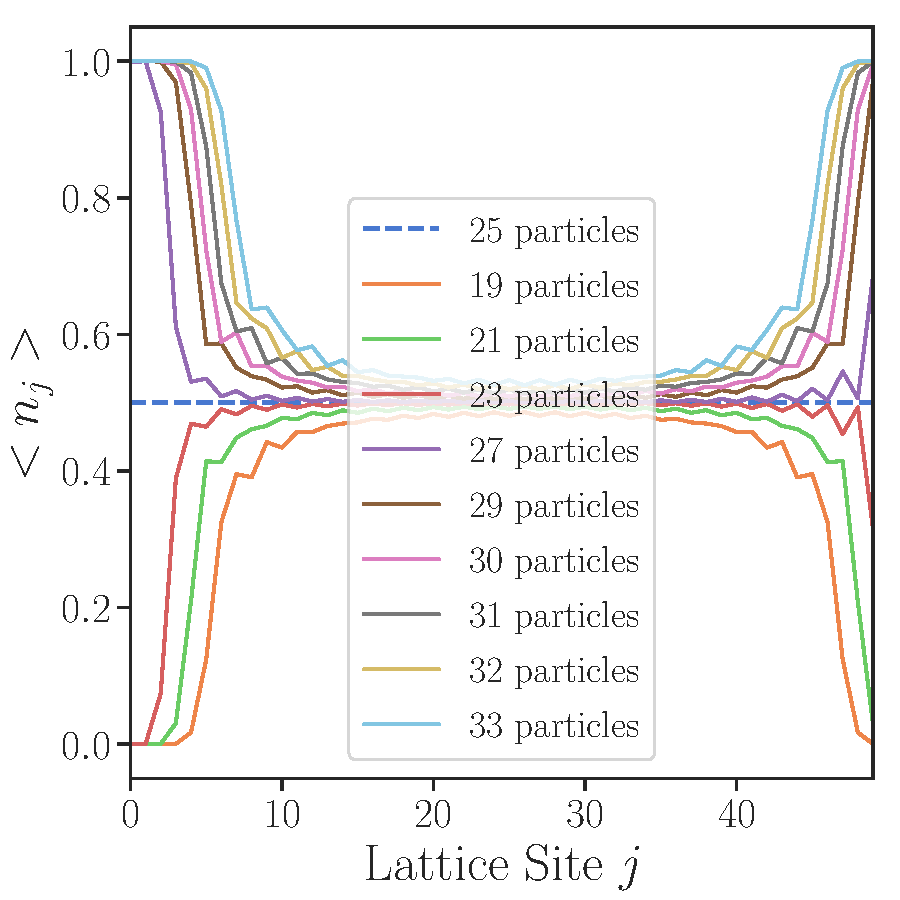
\includegraphics[width =\textwidth]{Occupation_number_H1}
	\caption{}
	\label{Occupation_number_H1}
\end{subfigure}
\caption{(a) Expectation Value of the Bond Energy in the Ground state with half filling as a function of the lattice site (b) The Occupation number $n_j(\epsilon_l) = \abs{\varphi_{l,i}}^2$ as a function of the energy index $l$ and the lattice site close to the chemical potential $\mu = 0$ for $L = 50$.}
\end{figure}	

 As can be seen in Fig. \ref{BondEnergy}, employing the sine-squared deformation to a tight-binding model greatly reduces the boundary modulations of the bond-energy $\expval{\hat{c}_j^\dagger\hat{c}_{j+1} + \hat{c}_{j+1}^\dagger \hat{c}_j}$ in the ground state for a half filled one-dimensional chain of size $L=100$. Furthermore, we observe that in the bulk of the system, the bond strength becomes translationally invariant. By investigating the occupation number $\expval{n_j} = \mel{G}{\hat{c}_j^\dagger \hat{c}_j}{G}$, we further observe that the variation in the total number of electrons, changes the edges of the system and leaves the bulk mainly unchanged. The results are shown in Fig. \ref{Occupation_number_H1}. Interestingly, for particle numbers smaller than the system size, the particles accumulate close to the center of the system and away from the edges. At the crossing to particle numbers larger than the system size, the excess particles start accumulating near the edges of the system \cite{Hotta}.  \\

%Nonetheless, quantities such as the bond energy and particle density obtained from the two-point correlation function, are translationally invariant
%
%
%Nonetheless, quantities such as the bond energy and particle density which are obtained from the two-point correlation function, share the same overall properties as the translationally invariant periodic boundary system.
%
%
%
%however nonetheless manages to create a position-independent two-point correlation function which shows translational invariance in the bulk of the system.  For periodic boundary conditions, the system is translationally invariant. Surprisingly, even though the sine-squared deformation breaks the translational invariance, it can be shown that they share the same \\



 
 
In addition to the different effects resulting from the choice of boundary conditions, we briefly note that they also share different finite-size error scaling behaviors. The finite size errors are defined to be the deviation from the expectation value of an observable in the thermodynamic limit. As was shown in Ref. \cite{Gendiar} and Ref. \cite{Gendiar2}, the finite size error correction for the ground state energy for OBC are $1/N$ and $1/N^2$ for PBC and SSD. This means that the finite-size corrections decreases faster for a system with periodic boundary conditions or sine-squared deformations than with open boundary conditions. The finite size errors are therefore expected to be negligible for the one-dimensional chain, but sizable for the square lattice model, due to the exponentially increasing numerical cost in scaling a system to large lattice sites in two-dimensions.   \\

\begin{figure}
\centering
\begin{subfigure}[t]{0.49\textwidth}
	\centering
	\includegraphics[width =\textwidth]{Eigenstates_ProfileH0}
	\caption{}
\end{subfigure}
\begin{subfigure}[t]{0.49\textwidth}
	\centering
	\includegraphics[width =\textwidth]{Eigenstates_ProfileSSD}
	\caption{}
	\label{fig:Eigenstates_ProfileSSD}
\end{subfigure}
\caption{Profile of the unnormalized eigenstates $|\varphi(l,j)|^2$ shown here for different energy levels $l$ as a function of $j$ for the (a) tight-binding Hamiltonian (b) sine-squared deformed Hamiltonian}
\label{fig:eigenstates_1d}
\end{figure}

%It can be shown that applying the sine-square deformation to the one-dimensional free fermion system with open boundary conditions completely removed unwanted boundary effects such as the Friedel oscillation. This resulted in position-independent two-point correlation functions such as the bond-strength and particle density/occupation number in the ground state (in the bulk of the system). 

%
%If one is interested in the bulk properties of the system, we wish to eliminate the  boundary effects as fast as possible. In addition to using PBC to suppress said effects, so-called smooth boundary conditions can be used, which turn of interactions smoothly at the edges of the system without linking sites at the opposite ends of the system.

%and therefore require a careful investigation on its effects on the observables. The resulting finite size errors, which are defined to be the deviation from the observed quantity in the thermodynamic limit, will be less of a problem numerically for the one-dimensional case but due the increasing computational constraint, scaling the two-dimensional square lattice system to large system sizes, is a more formidable task. 
%
%
%Often, periodic boundary conditions are imposed to suppress the boundary induced finite size effects, such as of Friedel oscillations, caused by open boundary conditions. 


%In general, solving a many-body quantum mechanical system involves understanding the physical properties of the bulk of the system. In general the measured bulk quantities are independent of the boundary condition. For finite systems finite size corrections of these boundary conditions however makes the choice of boundary condition relevant for the understanding of the bulk properties. This will be less of a problem numerically for the one-dimensional case but due to computational constraints, scaling a 2d dimensional system to higher lattice sites to minimize the finite-size error corrections is a formidable task. It is therefore important to study the effect of the boundary conditions on the physical properties of the system. \cite{Hotta} \\

%In finite systems such as the models treated in this thesis the choice of boundary conditions will have a direct effect on the properties of the system. In general, there are two choices of boundary conditions, periodic-boundary conditions and open-boundary conditions. In general, open boundary conditions introduce boundary oscillations such as Friedel oscillations,
%




\subsection{Sine-Square Deformation in momentum space}
In the $k$-Basis where the tight-binding Hamiltonian is diagonal, the chiral Hamiltonian takes the form:
\begin{equation}
	\hat{\mathcal{H}}^{(\pm)} = \sum_k e^{\mp i \delta/2} \epsilon(k \mp \delta/2) \hat{c}_k^\dagger \hat{c}_{k \mp \delta}
\end{equation}
The Hamiltonian includes terms that describe momentum transfers $\Delta k = \pm \delta$ only for nearest neighbor sites in $k$ space. Due to the Pauli exclusion principle, applying this Hamiltonian on the Fermi sea of the tight-binding model, restricts the possible momentum transfers to only include those across the Fermi point $k = \pm k_F$. It should therefore be evident, that the chiral Hamiltonian can generate excited states of $\hat{H}_{\text{tb}}$\cite{Hotta}. \\

If however, the chemical potential $\mu$ is fined-tuned such that $\epsilon(k_F \mp \delta/2) = 0$, no active excitation processes exist\footnote{In our one-dimensional numerical studies, setting $\mu = 0$ generated such a scenario}. Then, the Fermi sea of the tight-binding model with PBC is also an exact eigenstate of the chiral Hamiltonian \cite{Maruyama}.\\

\begin{figure}
\centering
\begin{subfigure}[t]{0.4\textwidth}
	\centering
	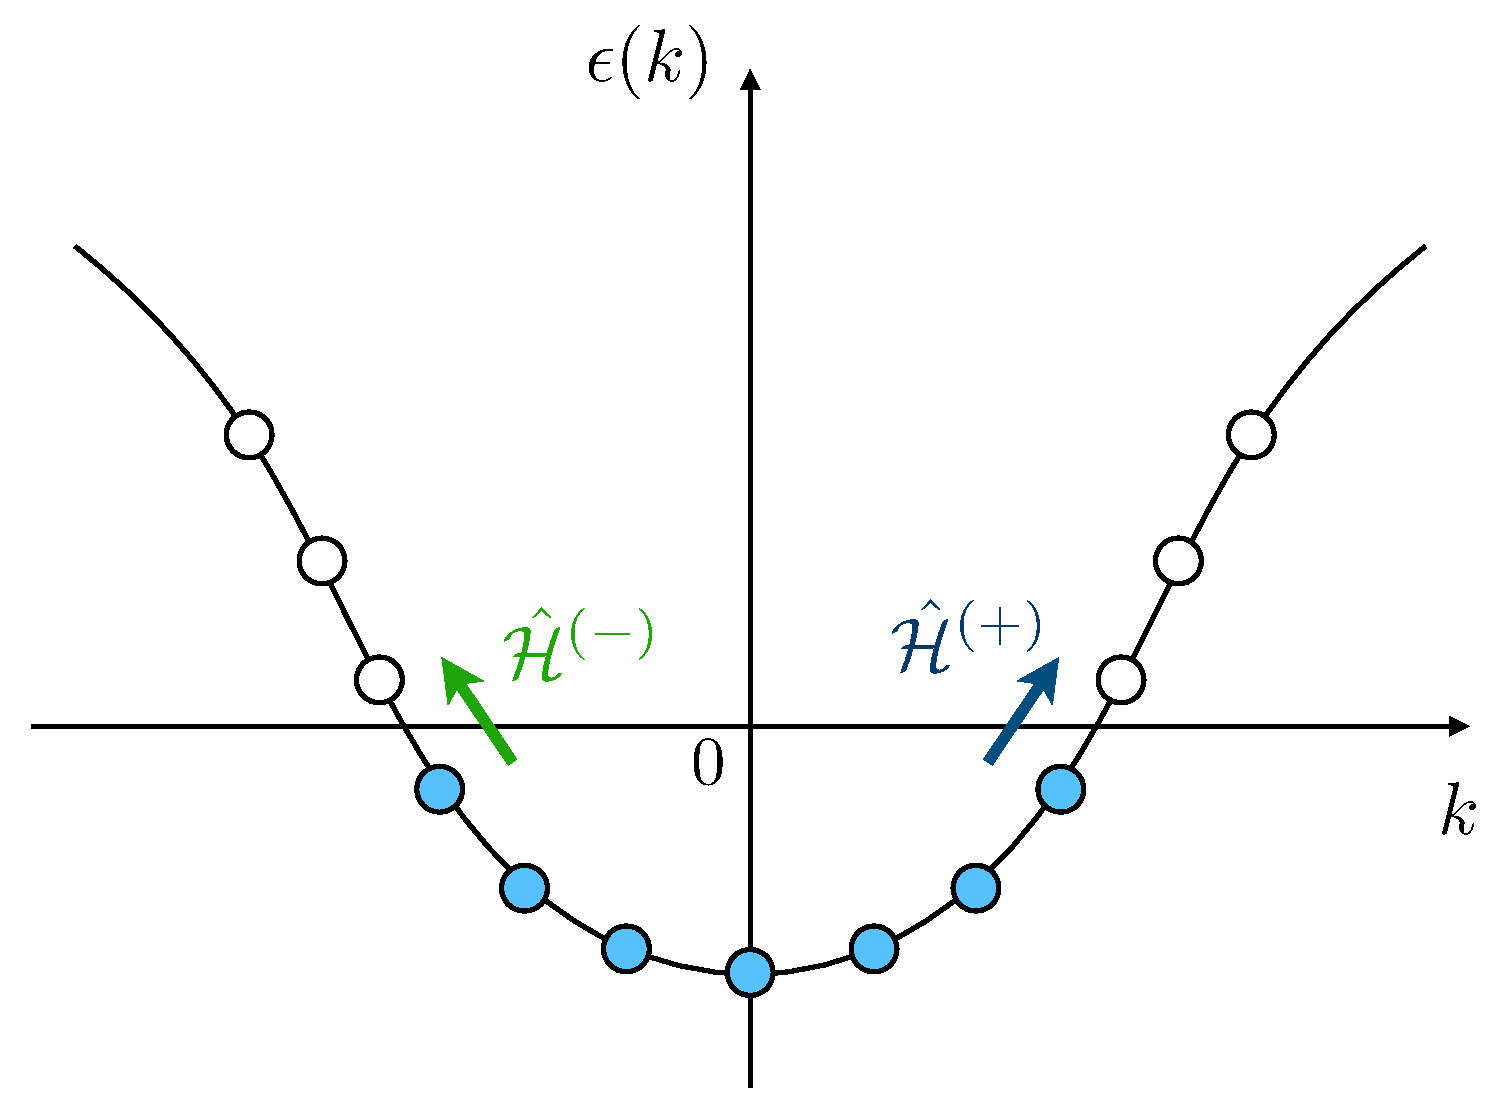
\includegraphics[width =\textwidth]{SSD_Construction}
	\caption{}
\end{subfigure}
\begin{subfigure}[t]{0.4\textwidth}
	\centering
	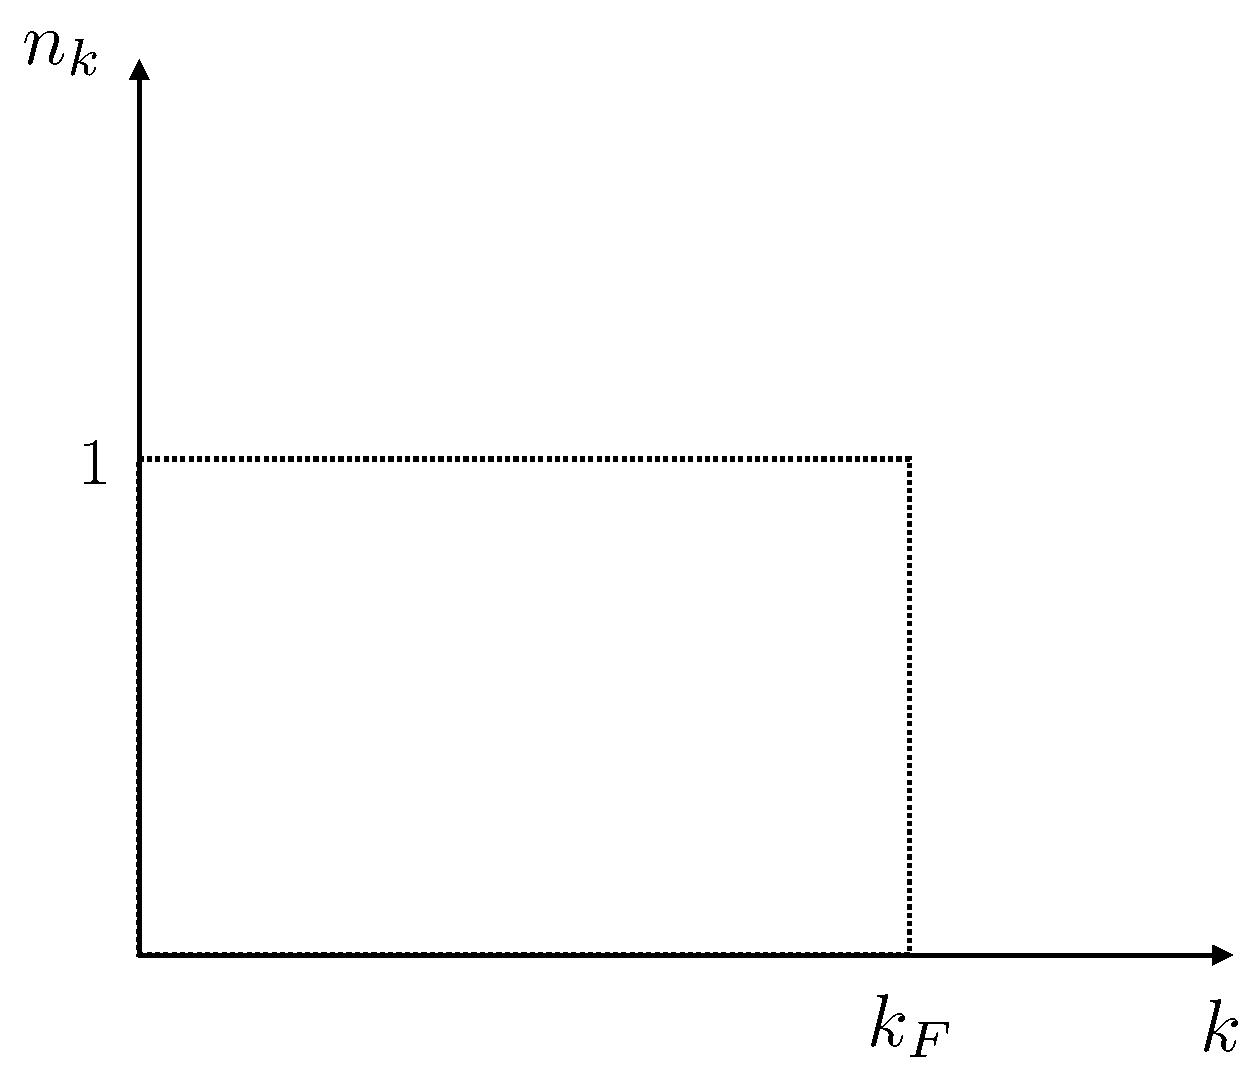
\includegraphics[width =\textwidth]{Disperion_relation1D}
	\caption{}
	\label{Fermi-Dirac-DistributionT=0}
\end{subfigure}
\caption{(a) Schematic representation of the allowed chiral $\hat{\mathcal{H}}^{(+)}$ (blue arrow) and anti-chiral $\hat{\mathcal{H}}^{(-)}$ (green arrow) excitations in momentum space. Due to the Pauli principle these processes are heavily restricted and only processes at the Fermi momentum $k_F$ are allowed (b) Occupation number for the ground state at zero temperature.}
\label{fig:dispersion_relation1D}
\end{figure}


More notable, it can be shown, that the Fermi sea is not only an exact eigenstate of the PBC system, but also corresponds to the exact ground state of the SSD Hamiltonian \cite{Katsura}\cite{Maruyama}. This is the reason, we observe that the SSD deformation recovers the translational symmetry of the PBC system. \\

The probability distribution of the eigenfunctions $\abs{\varphi(l,j)}^2$ are shown in Fig. \ref{fig:eigenstates_1d}. As expected, for the tight-binding model with periodic boundary conditions, the eigenfunctions are plane waves with different crystal momenta $k$. For the sine-squared Hamiltonian, the wave number $k$ is not a good quantum number anymore, due to the mixing term in the chiral Hamiltonian. We observe, that the eigenstates are rather a superposition of plane waves with different $k$ values\footnote{Also commonly referred to as a wave packet} localized at different locations in real space \cite{Hotta}. For increasing energies, the peaks of the wave packets shift left and right until around the zero energy level $\epsilon = \mu = 0$ (which for a half filled system, corresponds to $l = 500$ in Fig. \ref{fig:Eigenstates_ProfileSSD}), where the packets become localized around the edges of the system. With the help of the dispersion relation \ref{fig:dispersion_relation1D}, we can conclude, that eigenstates around the concentrated $\epsilon = \mu = 0$ level, correspond to localized edge states \cite{Hotta}. As was shown in \cite{Hotta}, the wave packets in the center have large energy and a light mass, forming the bulk of the system. The ones at the edges have a heavy mass and can hardly move, serving as reservoir or particle bath. This helps explains why changing the particle number incrementally around the $N_g = L/2$ value, only drastically changes the particle density near the system edges (as seen in Fig. \ref{Occupation_number_H1}) but maintains the optimal value\footnote{corresponding to the value obtained in a PBC system at the thermodynamic limit} in the bulk \cite{Hotta}.
\begin{figure}[h]
\centering
\begin{subfigure}[t]{0.49\textwidth}
	\centering
	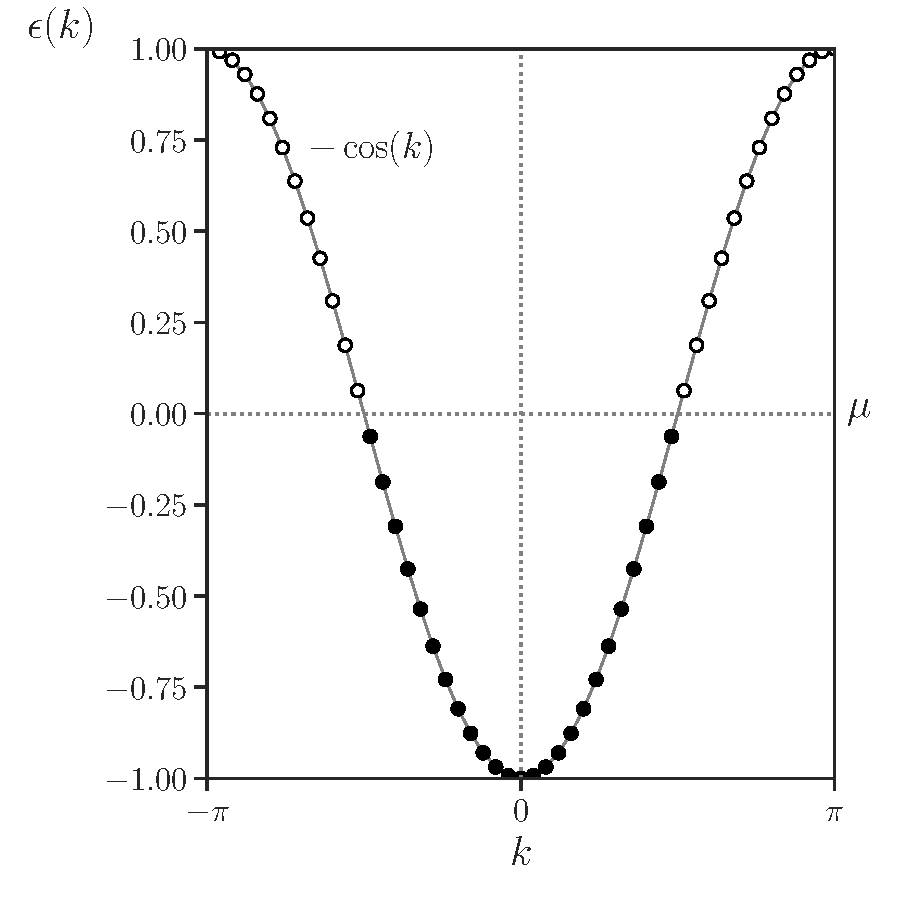
\includegraphics[width =\textwidth]{dispersionrelationH0}
\end{subfigure}
\begin{subfigure}[t]{0.49\textwidth}
	\centering
	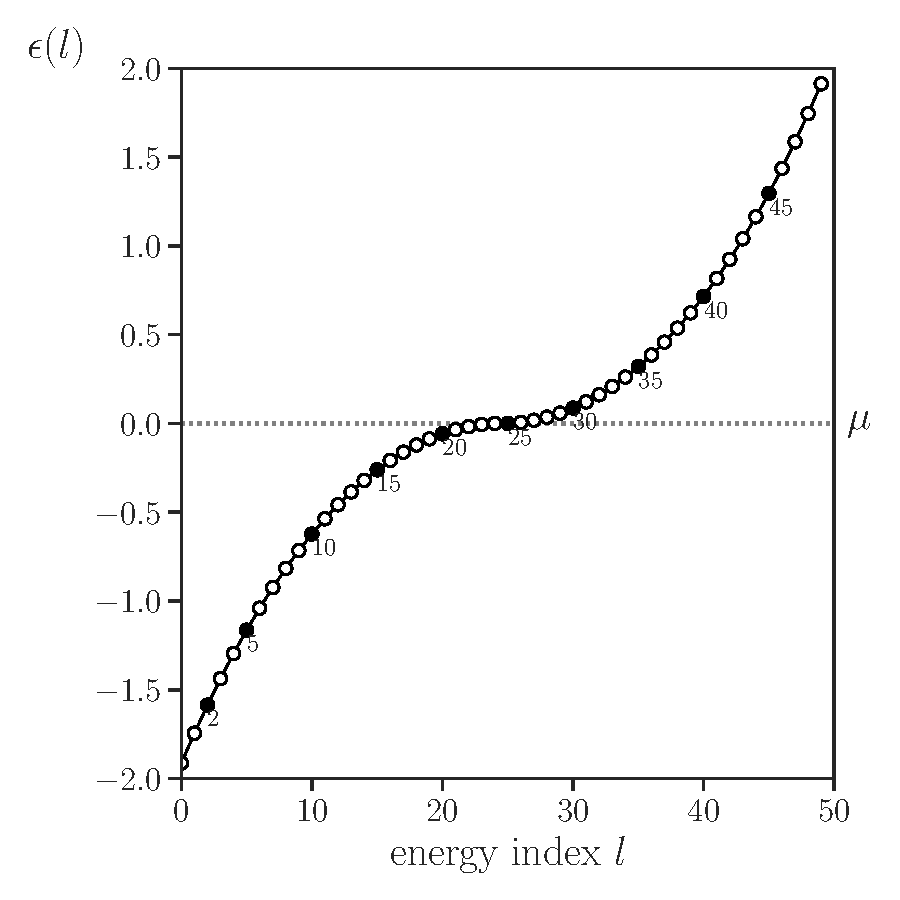
\includegraphics[width =\textwidth]{dispersionrelationSSD}
\end{subfigure}
\caption{(left) Dispersion relation $\epsilon(k) = -2t\cos(ka)$ for the tight-binding Hamiltonian for $L=50$, chemical potential $\mu = 0$, lattice constant $a = 1$ and hopping parameter $t = 1/2$. Represented is the half-filled ground state occupation up to the Fermi level $\epsilon_F = \mu =0$ for spinless fermions. (right) energy-eigenvalues for the sine-squared deformed Hamiltonian $\hat{H}_{\text{SSD}}$ for $L = 50$ and $\mu = 0$.}
\label{fig:dispersion_relation1D}
\end{figure}




\subsubsection{In two-dimensions}
The construction of the sine-squared deformed Hamiltonian in two-dimensions for a square lattice follows analogously to the one-dimensional case with the introduction of a chiral Hamiltonian \cite{Maruyama}:
\begin{equation}
\begin{split}
	\hat{H}^{(\pm)} = & \sum_{\mathbf{r}}\Big( -\frac{t_1}{2}  \exp(\pm i[\delta_x x + \delta_y( y - 1/2)]) \left[\hat{c}^\dagger(x,y) \hat{c}(x+1, y) + \text{h.c}\right] \\
		&- \frac{t_2}{2} \exp(\pm i [\delta_x(x-1/2) + \delta_y y]) \left[\hat{c}^\dagger(x,y) \hat{c}(x, y+1) + \text{h.c} \right] \Big)
\end{split}
\end{equation}
where $t_1$ corresponds to the hopping in $x$-direction and $t_2$ in $y$-direction. Similarly, the diagonal chiral Hamiltonian in momentum space is:
\begin{equation}
	\hat{\mathcal{H}}_{\bm{\delta}}^{(\pm)} = \sum_{\mathbf{k}} e^{\mp i/2(\delta_x + \delta_y)} \epsilon(\mathbf{k} + \bm{\delta}/2)\hat{c}_{\mathbf{k}}^\dagger \hat{c}_{\mathbf{k} \mp \bm{\delta}}
\end{equation}
which again describes the active processes connecting the sites $\mathbf{k}$ and $\mathbf{k} \pm \bm{\delta}$. The difference to the 1d case however here is that $\epsilon(\mathbf{k} + \bm{\delta}/2) = 0$ cannot be achieved by tuning the parameter $\mu$ which means that the Fermi sea is only an approximate eigenstate of the chiral Hamiltonian and an exact correspondence is only achieved in the thermodynamic limit $L_{x,y} \rightarrow \infty$\cite{Maruyama}. The sine squared Hamiltonian in the two-dimensional case is then constructed analogously to the one-dimensional case with $\hat{H}_{\text{SSD}} = \hat{H}_0/2 - [\hat{H}^{(+)} + \hat{H}^{(-)}]/4$:
\begin{equation}
\begin{split}
\hat{H}_\text{SSD} = \sum_{i=1}^{L_x} \sum_{j=1}^{L_y} & \Big(t_1 \mathcal{F}\left(x+\frac{1}{2}, y\right) \left[ \hat{c}^\dagger(x,y)\hat{c}(x+1, y) + \hat{c}^\dagger(x+1,y) \hat{c}(x,y)\right] \\
&+ t_2 \mathcal{F}\left(x, y+ \frac{1}{2}\right) \left[\hat{c}^\dagger(x, y) \hat{c}(x, y + 1) + \hat{c}^\dagger(x, y+1) \hat{c}(x,y) \right] \Big)
\end{split}
\label{eq:SSD_Hamiltonian2D}
\end{equation}
where we used to following modified function for our deformation:
\begin{equation}
	\mathcal{F}(x,y) = f_x(x)f_y(y) = 4\sin(\frac{\pi x}{L})^2\sin(\frac{\pi y}{L})^2
	\label{eq:sine_squared_deformation2d}
\end{equation}
This expression is best generalized as a sum over the two index coordinate tuple $(i, j)$, as done in equation (\ref{eq:tight_binding_2d_Hamiltonian}):
\begin{equation}
	\begin{split}
		\hat{H}_\text{SSD} = \sum_{i=1}^{L_x-1} \sum_{j=1}^{L_y-1} & \Big(t_1 \mathcal{F}\left(i+\frac{1}{2}, j\right) \left[ \hat{c}^\dagger(i,j)\hat{c}(i+1, j) + \hat{c}^\dagger(i+1,j) \hat{c}(i,j)\right] \\
&+ t_2 \mathcal{F}\left(i, j + \frac{1}{2}\right) \left[\hat{c}^\dagger(i, j) \hat{c}(i, j + 1) + \hat{c}^\dagger(i, j+1) \hat{c}(i,j) \right]\Big)
	\end{split}
\end{equation}





\subsection{Evolution of ground state from PBC to SSD}
In this section, we aim to analyze how the ground state of the PBC system changes, if we apply a sine-squared deformation, similarly to the analysis done in Ref \cite{Maruyama}. This was done by introducing the toy-Hamiltonian:
\begin{equation}
	\hat{H}(a) = (1-a)\hat{H}_\text{tb} + a \hat{H}_{\text{SSD}}
\end{equation}
with the variable parameter $a =[0,1]$. For $a=0$ we recover the Hamiltonian with PBC conditions and for $a=1$ we obtain the SSD Hamiltonian. For simplicity, we replace the deformation function $\mathcal{F}(x,y)$ in the SSD Hamiltonian (\ref{eq:SSD_Hamiltonian2D}) by:
\begin{equation}
	\mathcal{F}(x,y) \rightarrow \mathcal{F}(x;a) = (1-a) + af_x(x) 
\end{equation}
where $f_x(x)$ corresponds to the function defined in equation (\ref{eq:scaling_function_SSD}). In Fig. \ref{EvolutionEnergies1D} we observe that for a half-filled one-dimensional lattice, the ground state for $a=0$ is also a ground state for $a=1$. However as can be seen in \ref{EvolutionEnergies2D}, for the two-dimensional system, this is not the case since at around $a = 0.69$ we observe a level crossing over the Fermi Energy $E_F = \mu =0$, meaning the number of particles with $E<0$ changes and the Fermi sea at $a=0$ is not the ground state for $a=1$, but an excited state. Furthermore, we note, that in both one-dimension and in two-dimension, the sine-squared deformation changes the degeneracy of the eigenstates \cite{Maruyama}.

\begin{figure}[h]
\begin{subfigure}{.5\textwidth}
  \centering
  \includegraphics[width=\linewidth]{EvolutionEnergies1D.pdf}
  \caption{}
  \label{EvolutionEnergies1D}
\end{subfigure}
\begin{subfigure}{.5\textwidth}
  \centering
  \includegraphics[width=\linewidth]{EvolutionEnergies2D.pdf}  
  \caption{}
  \label{EvolutionEnergies2D}
\end{subfigure}
\caption{(a) Evolution of the energy eigenvalues for the one-dimensional lattice with $L = 10$, (b) Evolution of energy eigenvalues for the two-dimensional square lattice with $L_x = L_y = 5$.}
\end{figure}




%To observe the change of the ground state of a system with PBC once the SSD is applied, we introduce the toy hamiltonian \cite{Maruyama}:






%\begin{figure}[h]
%	\centering
%	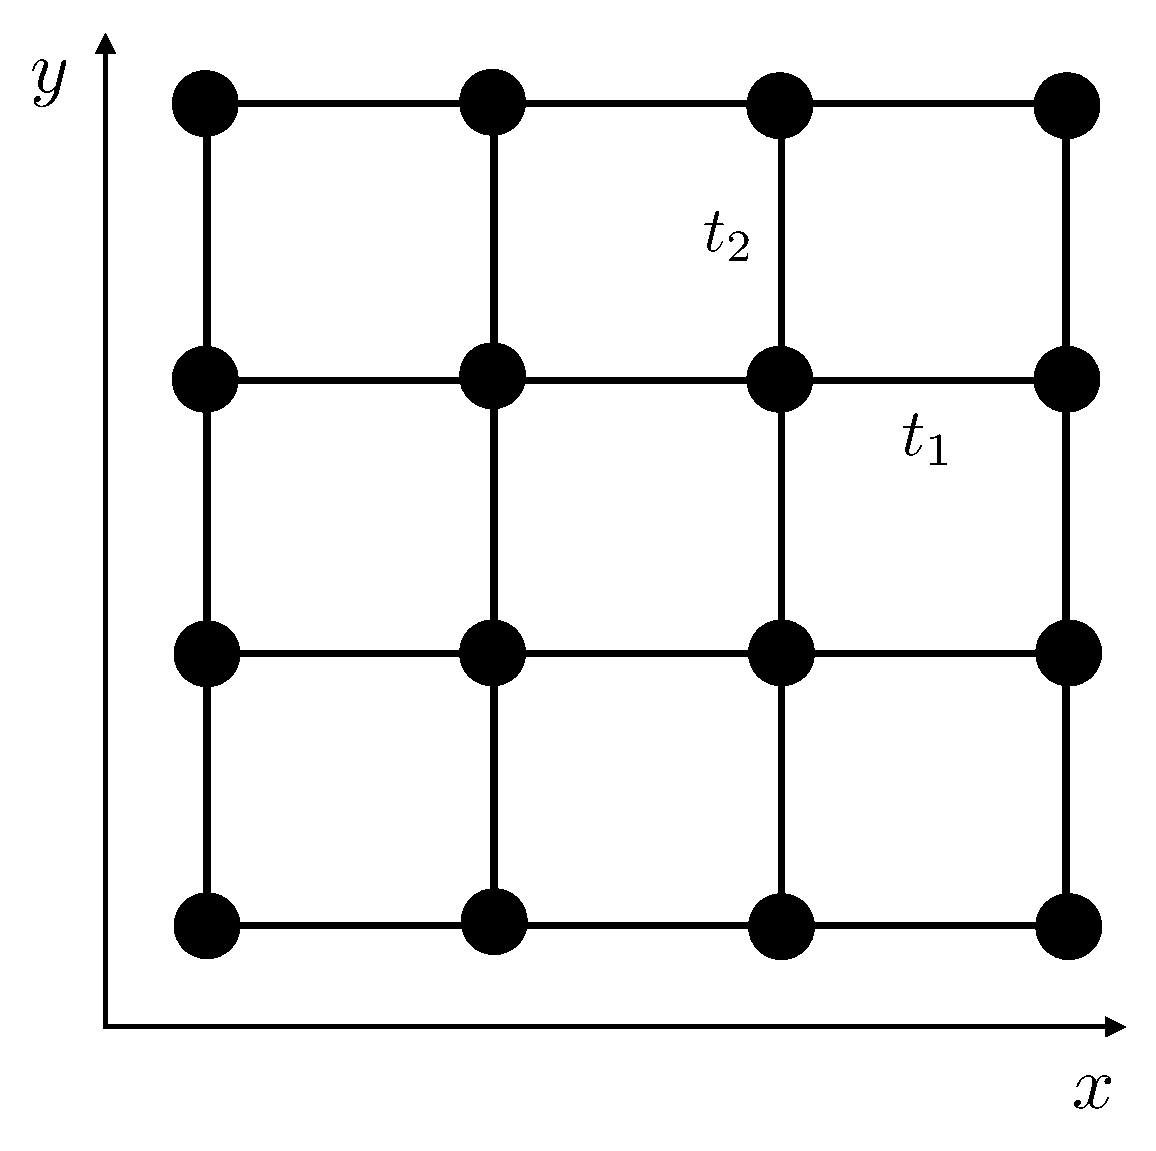
\includegraphics[width = 0.4\textwidth]{Square_Lattice}
%	\caption{}
%\end{figure}

%\begin{figure}
%	\centering
%	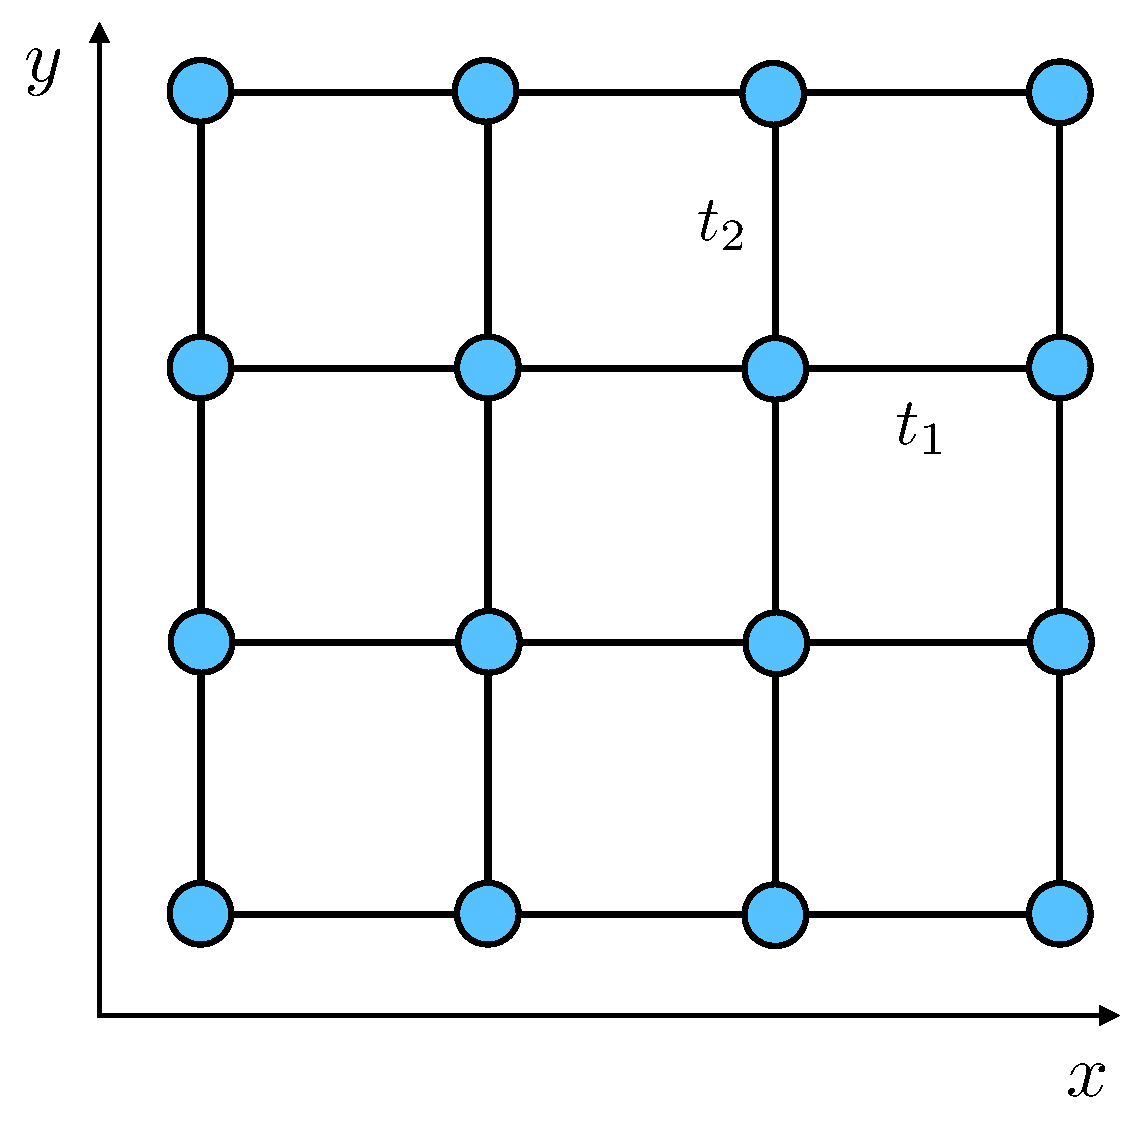
\includegraphics[width = 0.8\textwidth]{Square_Lattice2}
%	\caption{}
%\end{figure}

%\subsubsection{Energy corrections}
%
%For open boundary conditions the ground state energy at half filling is obtained by summing up all the negative eigenvalues:
%\begin{equation}
%	E_O^{N} = \sum_{i = 1}^{N/2} \epsilon_m = t\left[1 - \left(\sin(\frac{\pi/2}{N+1}) \right)^{-1} \right]
%\end{equation}
%The subscript in this case will denote the different possible cases, $O$ for OBC, $P$ for PBC and $S$ for SSD.
%Expanding the right hand side with respect to $N$, one finds the form
%\begin{equation}
%	\frac{E_O^N}{N} \sim - \frac{2 t}{\pi} + \frac{t}{N}\left( \frac{2}{\pi} - 1\right) + \mathcal{O}\left(\frac{1}{N^2}\right)
%\end{equation}
%Compared with the energy per site in the thermodynamic limit:
%\begin{equation}
%	\lim_{N \rightarrow \infty} \frac{E_O^N}{N} = \frac{1}{\pi} \int_{0}^{\pi/2} -2t \cos(k) \dd k = - \frac{2}{\pi} t 
%\end{equation}
%where we chose the integration limit to be from 0 to $\pi/2$ to include all $k$-modes with negative Energies in the case for $N \rightarrow \infty$. That this holds can be seen from the dispersion relation. The finite-size correction to the energy per site (or even the energy per bond) is of the order of $1/N$.
%
%
%It is expected that the ratio $E_S^N/ B^N$ rapidly converges to $-2t/\pi$ which is the expectation value $\expval{c_j^\dagger c_{j+1}^\dagger + \hat{c}_{j+1}^\dagger \hat{c}_j}$ in the thermodynamic limit, which in the case of $t = -1/2$ corresponds to the $0.636$ seen in the plot (\ref{BondEnergy}) 
%%\begin{equation}
%%	
%%\end{equation}
%
%
%%\begin{equation}
%%	\mel{0}{\hat{c}_m}{i} = \frac{1}{\sqrt{N}} \exp[i
%%\end{equation}

%\begin{equation}
%	\psi_
%\end{equation}


%	\begin{figure}[h]	
%		\centering
%		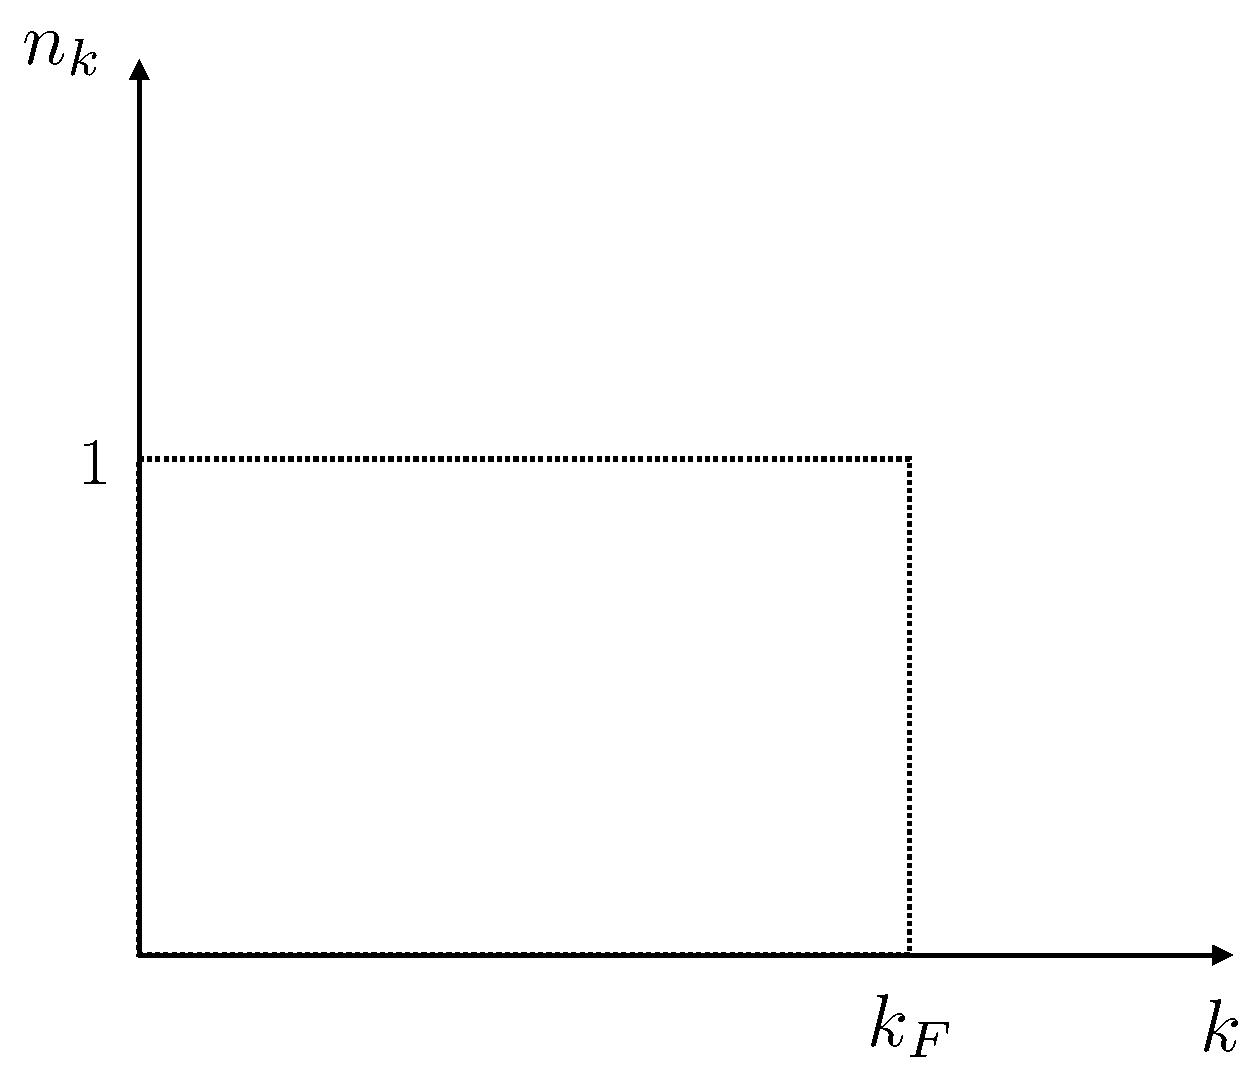
\includegraphics[width=0.8\textwidth]{Disperion_relation1D}
%		\caption{Dispersion relation and Occupation for a free fermion system (without spins) in one-dimension}
%	\end{figure}
%	

%\newpage
  
\section{Time evolution and Floquet theory}
In this section, we aim to introduce the Floquet framework, which will serve as the theoretical basis, in understanding the Floquet systems treated in this thesis. In general terms, Floquet theory investigates the behavior of quantum systems with time-dependent Hamiltonians satisfying the periodicity constraint: 
	\begin{equation}
		\hat{H}(t) = \hat{H}(t+ T)
	\end{equation}
Here $T$ denotes the period of the driving cycle\footnote{Evidently, all Floquet systems are therefore invariant under time translation}. The dynamics of a quantum system are fully captured in the time-dependent Schrödinger equation:
	\begin{equation}
		i\hbar \dv{t} \ket{\psi(t)} = \hat{H}(t) \ket{\psi(t)}
	\end{equation}
which can analogously be written in terms of the time-evolution operator $\hat{U}(t,t_0)$:
	\begin{equation}
		\ket{\psi(t)} = \hat{U}(t,t_0) \ket{\psi(t_0)}
	\end{equation}
The periodicity of the Hamiltonian is equivalent to the time-evolution operator satisfying:
\begin{equation}
	\hat{U}(t + T, t_0 + T) = \hat{U}(t, t_0)
\end{equation}
In the following, we will simply notation by choosing $t_0 = 0$ and setting $\hat{U}(t, t_0) = \hat{U}(t)$. In general, the time-dependent Hamiltonian will not commute with itself at different times, i.e  $\comm*{\hat{H}(t)}{\hat{H}(t')} \neq 0$ and the time-evolution operator has to be written as a time-ordered series\footnote{Also referred to as Dyson expansion}:
	\begin{equation}
	\begin{split}	
	\hat{U}(t) &= \mathcal{T} \exp(	-\frac{i}{\hbar} \int_{t_0}^t \dd t' \hat{H}(t'))\\
	&= \mathbbm{1} + \left(- \frac{i}{\hbar}\right) \int_{t_0}^t \dd t_1 \hat{H}(t_1) + \left(-\frac{i}{\hbar}\right)^2 \int_{t_0}^t \dd t_1 \hat{H}(t_1) \int_{t_0}^{t_1} \dd t_2 \hat{H}(t_2) + \dots
	\end{split}
	\label{eq:time_evolution_operator}
	\end{equation}
	where $\mathcal{T}$ stands for the time-ordered product. This guarantees that the $n$-th term in the Dyson expansion corresponds to the ordered product $\hat{H}(t_1)\hat{H}(t_2)\dots \hat{H}(t_n)$ of non-commuting Hamiltonians \cite{Santoro}. 





%\begin{figure}[h]
%    \centering
%    \subfigure[]{\includegraphics[width=0.24\textwidth]{ColorMapMatrix_PBC}} 
%    \subfigure[]{\includegraphics[width=0.24\textwidth]{ColorMapMatrix_OBC}} 
%    \subfigure[]{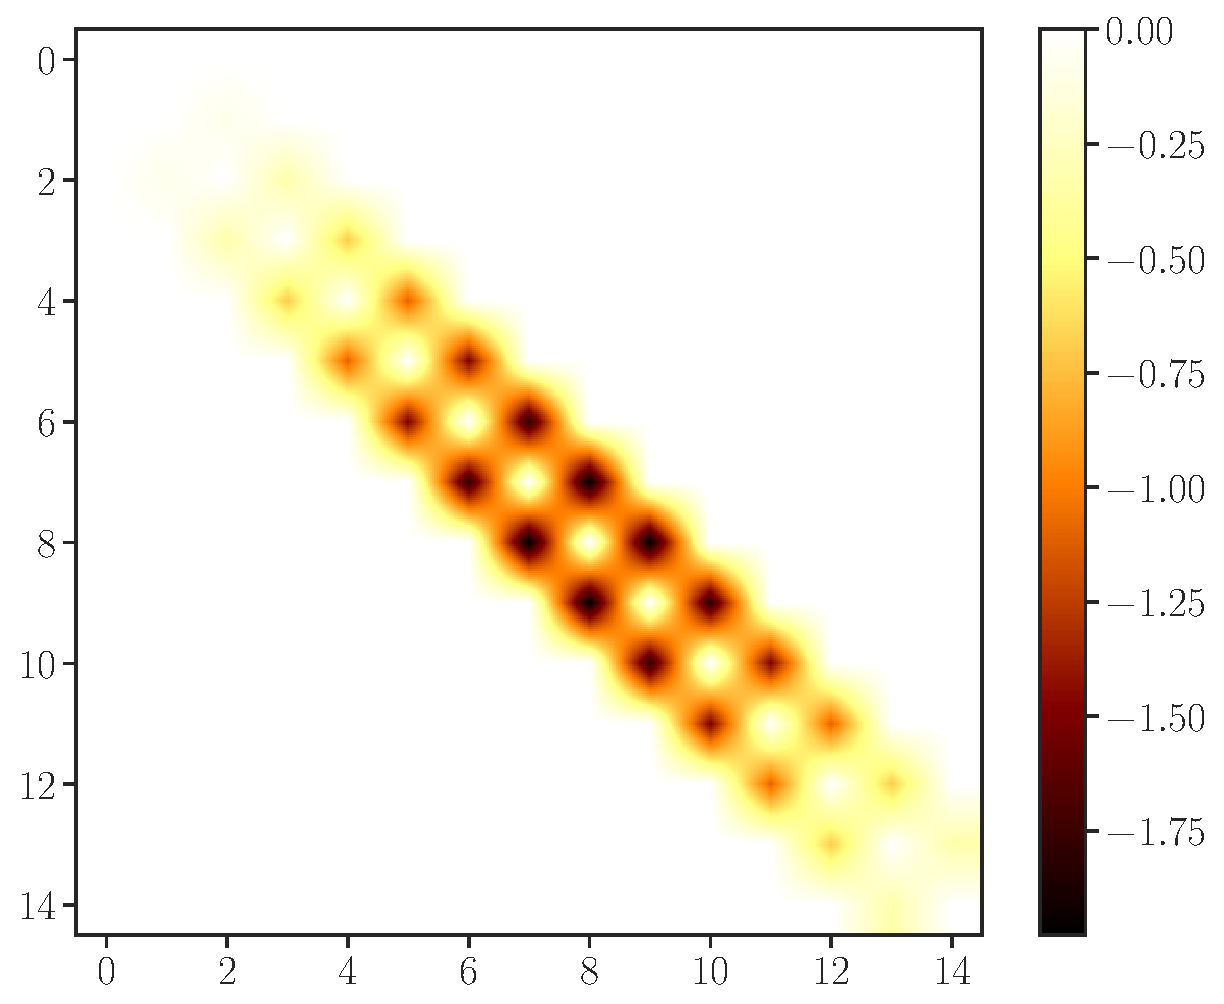
\includegraphics[width=0.24\textwidth]{ColorMapMatrix_SSD}}
%    \caption{(a) blah (b) blah (c) blah (d) blah}
%    \label{fig:foobar}
%\end{figure}

%\begin{figure}[H]
%   \subfloat[\label{genworkflow}]{%
%      \includegraphics[trim=20 40 50 30,clip, width=0.3\textwidth]{ColorMapMatrix_PBC}}
%\hspace{\fill}
%   \subfloat[\label{pyramidprocess} ]{%
%      \includegraphics[trim=10 40 10 30,clip, width=0.3\textwidth]{ColorMapMatrix_OBC}}
%\hspace{\fill}
%   \subfloat[\label{mt-simtask}]{%
%      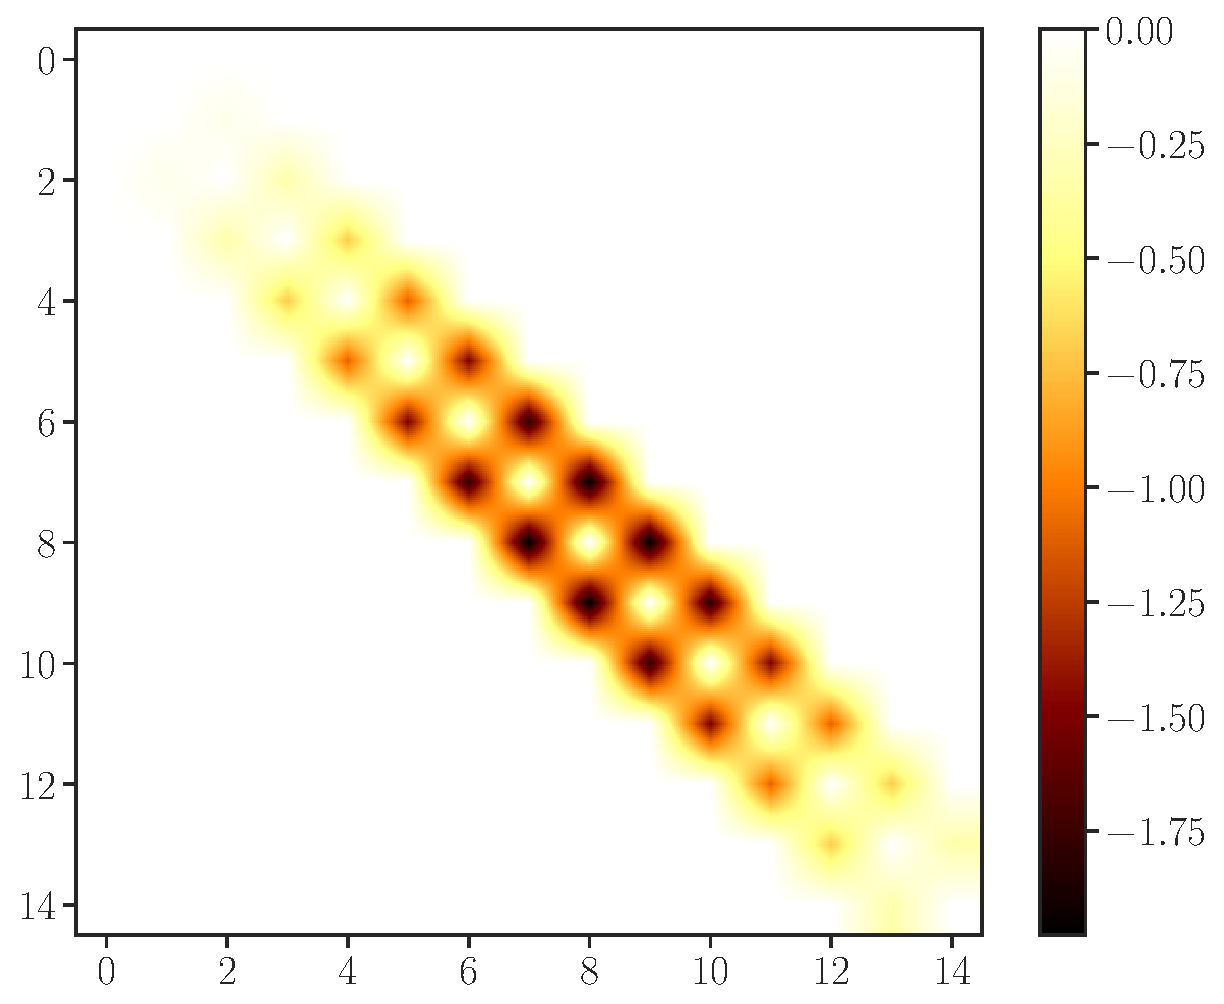
\includegraphics[trim=30 40 30 30,clip, width=0.3\textwidth]{ColorMapMatrix_SSD}}\\
%\caption{\label{workflow}The overall approach. (a) figa; (b) Workflow for figb; (c) Workflow for figc.}
%\end{figure}

%\begin{figure}
%	\centering
%	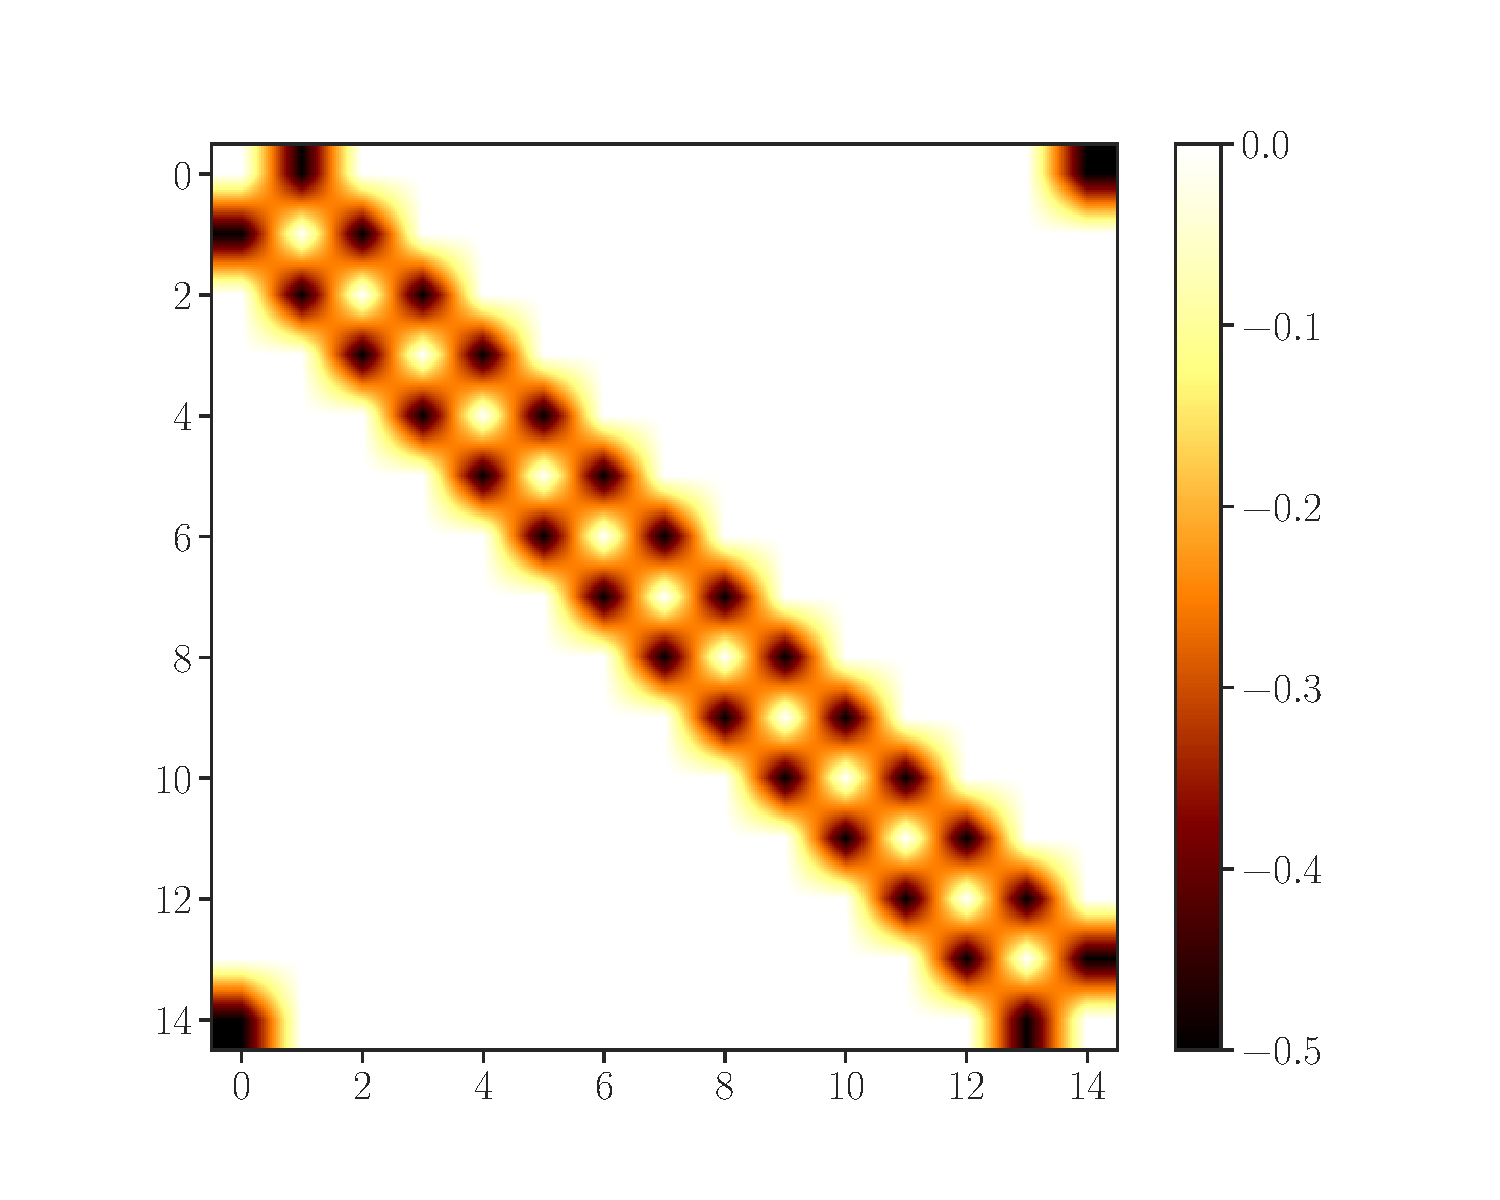
\includegraphics[width = 0.8\textwidth]{ColorMapMatrixH0_PBC}
%\end{figure}


%\begin{figure}[h]
%	\centering
%	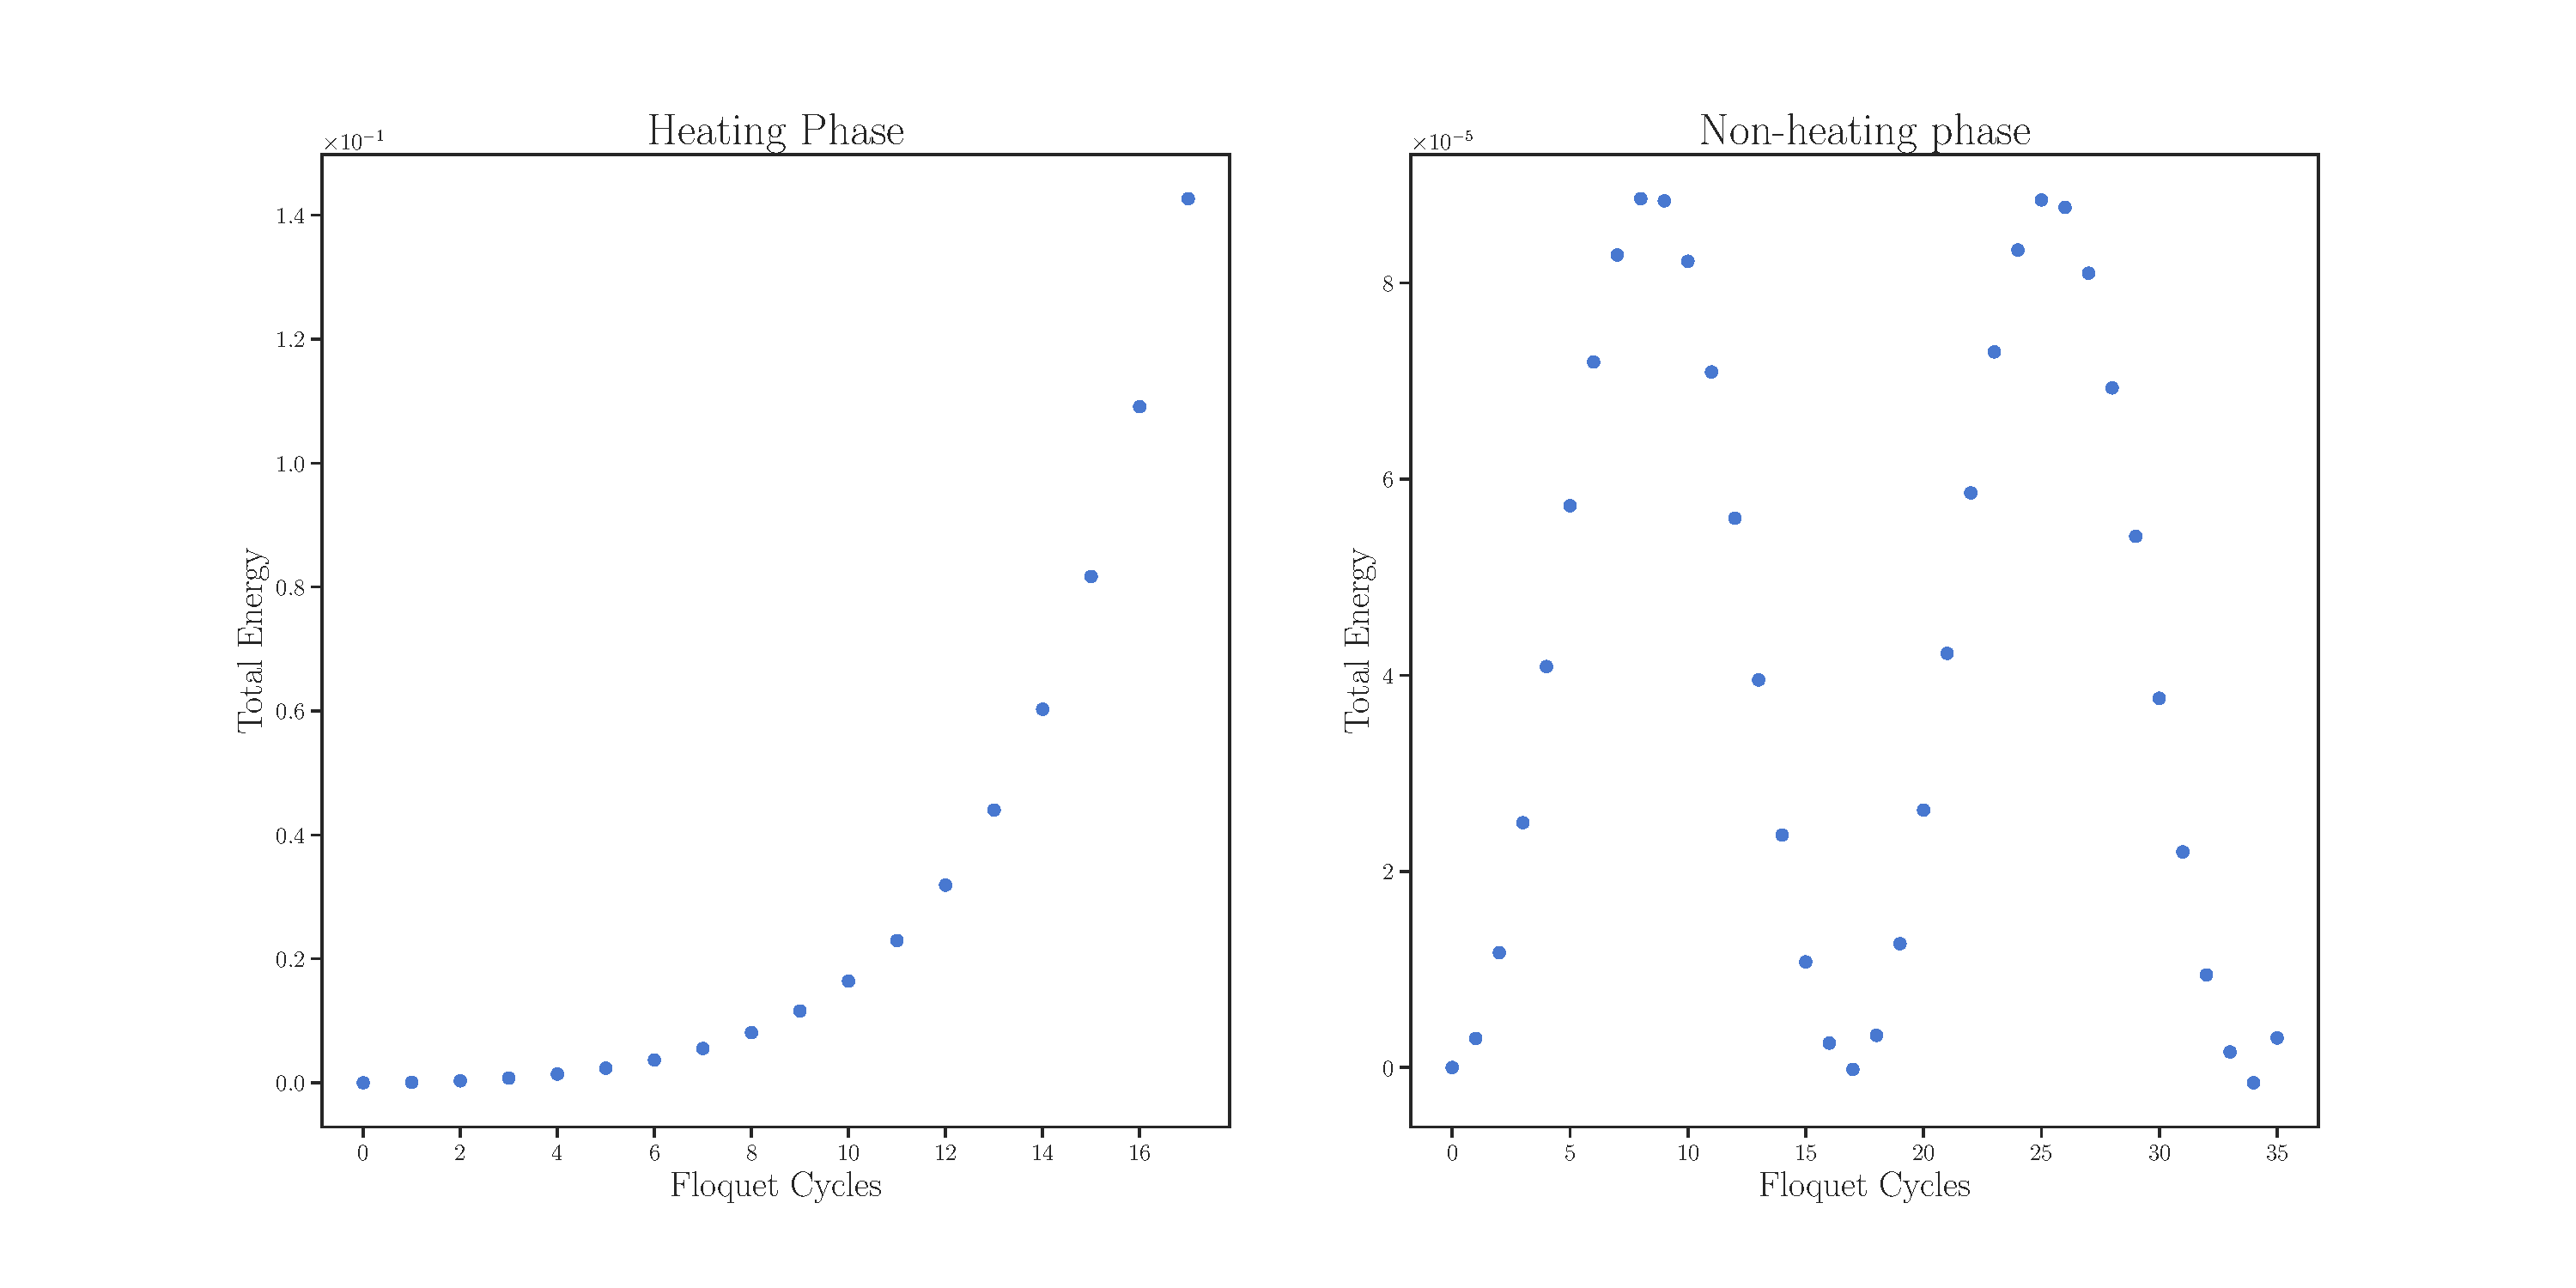
\includegraphics[width=1\textwidth]{Total_Energy1d}
%\end{figure}




\chapter{Floquet system in one-dimension}
Floquet systems have become a popular way to study statistical dynamics beyond equilibrium \cite{Andersen}. However, very few analytically solvable Floquet systems are available and the setting necessary for the formation of phases is not well understood. Generally, the periodic driving of a Floquet system, results in heating up the system towards a featureless infinite temperature state in which no notion of distinct phases can be observed \cite{Potter}. \\

 One analytically solvable Floquet system with a novel phase structure was proposed in a Paper published by Wen and Wu in 2018 \cite{Xueda}, in which the Floquet dynamics of the system were captured by a $(1+1)$-dimensional (periodically bulk driven) conformal field theory. On a lattice, such a system is best modeled with the free fermion chain at half filling and the time-dependent Hamiltonian:
	\begin{equation}
	\hat{H}(t) = 
		\begin{dcases}
		\hat{H}_\text{1} = \sum_{i=1}^{L-1} \sin^2\left( \frac{\pi(i + 1/2)}{L}\right) \left[ \hat{c}_i^\dagger c_{i+1} + \hat{c}_{i+1}^\dagger \hat{c}_i \right] \quad &0<t< T_1 \\
		\hat{H}_0 = \frac{1}{2} \sum_{i=1}^{L-1} [\hat{c}_i^\dagger \hat{c}_{i+1} + \hat{c}_{i+1}^\dagger \hat{c}_{i} + \alpha ( \hat{c}_{L}^\dagger \hat{c}_1 + \hat{c}_1^\dagger \hat{c}_L)]  &T_1 < t < T_1 + T_0
		\end{dcases}
		\label{eq:Floquet_Hamiltonian1d}
	\end{equation}
where the transition amplitude is set to $t=1$ and $\alpha = \{1,0\}$ determines the imposed boundary condition. The initial state of the system is chosen to be the ground state $\ket{G}$ of $\hat{H}_0$.
\begin{figure}[h]
\centering
		\begin{subfigure}[b]{0.45\textwidth}
			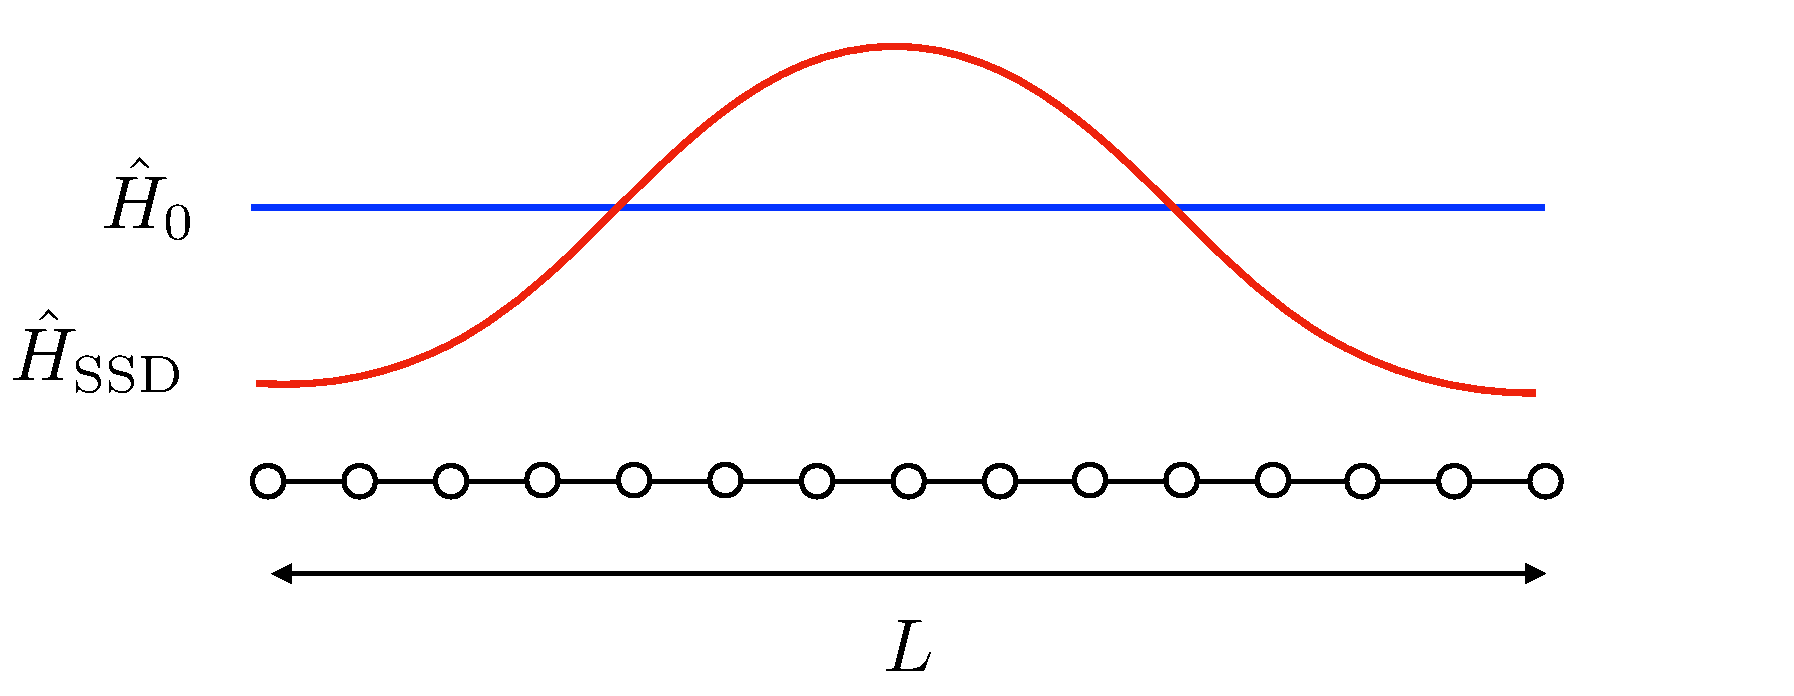
\includegraphics[width=\textwidth]{Floquet_Drive1D_Deformation.pdf}
			\caption{}
		\end{subfigure}
		\begin{subfigure}[b]{0.45\textwidth}
			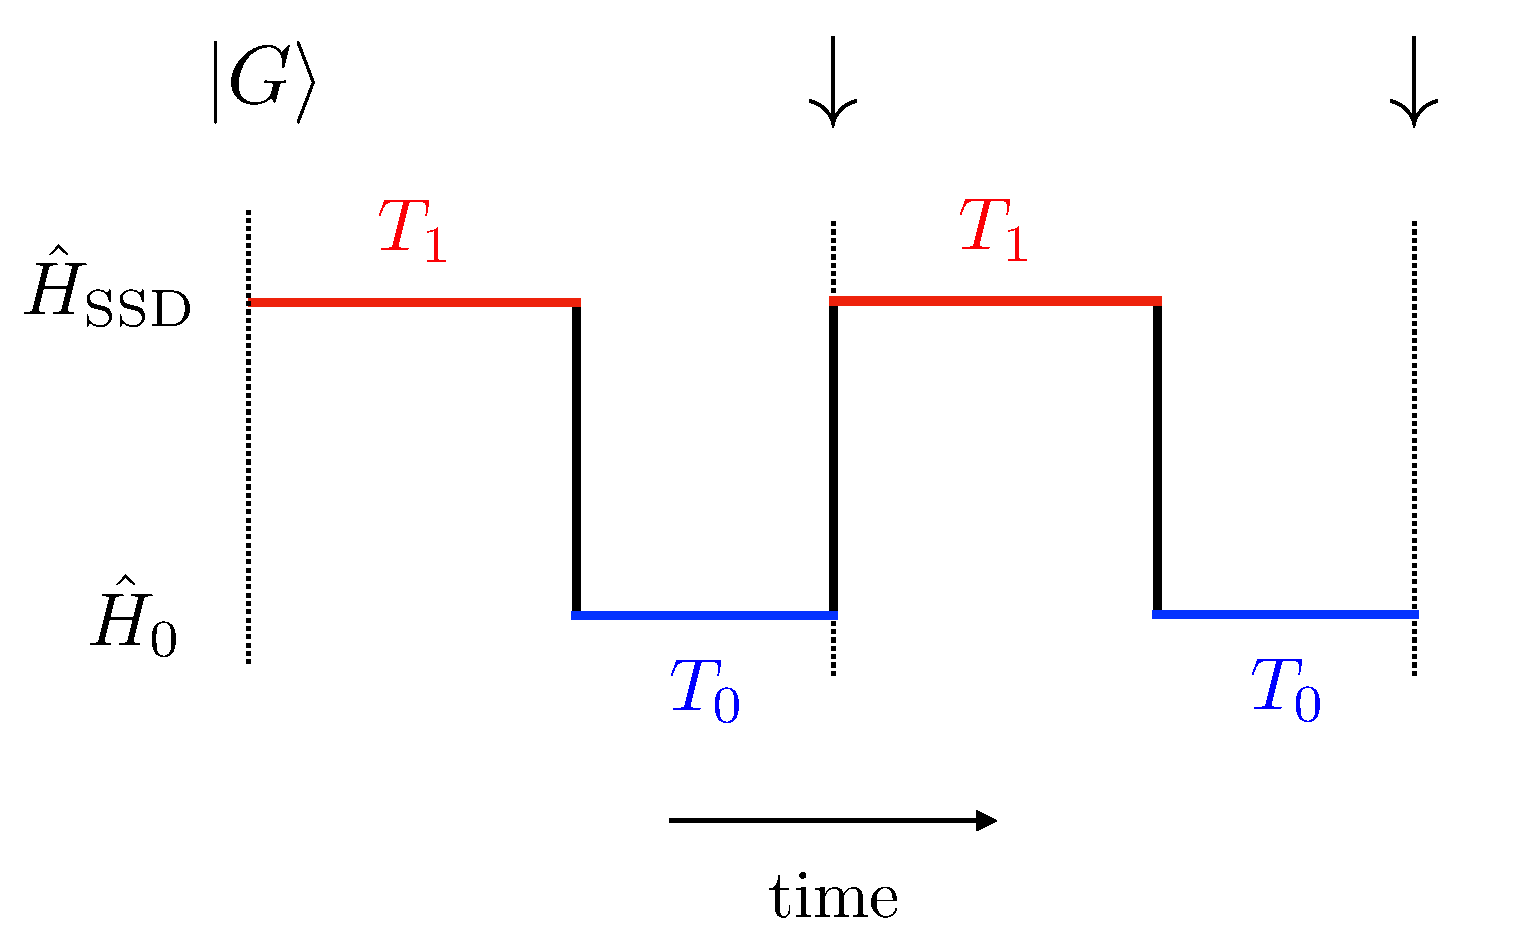
\includegraphics[width=0.95\textwidth]{Floquet_Drive.pdf}
			\caption{}
		\end{subfigure}
		\caption{(a) Hamilton densities for the tight-binding Hamiltonian and SSD deformation (b) The Floquet drive, where the black arrows indicate stroboscopic times.}
		\label{fig:Floquet_system_1d}
\end{figure}
 Then for time $T_1$, we evolve the state with $\hat{H}_1$, followed by an evolution with $\hat{H}_0$ for time $T_0$, to complete one cycle $T = T_0 + T_1$. For this step-wise, one cycle, driving protocol, the time-evolution operator \ref{eq:time_evolution_operator} simplifies to the following form: 
\begin{equation}
	\hat{U}(T) = \mathcal{T}\exp(-i \int_{0}^T \hat{H}(t) \dd t') = e^{-i \hat{H}_0 T_0} e^{-i \hat{H}_1 T_1}
	\label{eq:time_evolution_operator1d}
\end{equation}
The resulting time-evolved state $\ket{\psi(t)}$ is $\ket{\psi(T)} = \hat{F}(T) \ket{G}$, where we defined the Floquet operator $\hat{F}(T)$, which corresponds to the time-evolution operator over one period. The state $\ket{\psi(nT)}$ after $n$-cycle driving is then given by:
\begin{equation}
	\ket{\psi(nT)} = \hat{F}(nT) \ket{G}
\end{equation}
where similarly to \ref{eq:time_evolution_operator1d}, the Floquet operator is given by:
\begin{equation}
\begin{split}
		\hat{F}(nT) = \mathcal{T} \exp(-i \int_{0}^{nT} \hat{H}(t') \dd t') &= e^{-i \hat{H}_0 T_0}e^{i \hat{H}_1 T_1}\dots e^{-i \hat{H}_0 T_0} e^{-i\hat{H}_1 T_1} \\
		&= \left( e^{-i \hat{H}_0 T_0} e^{-i \hat{H}_1 T_1} \right)^n
\end{split}
\label{eq:Floquet_operator_n_cycles}
\end{equation}
The dynamical characterization of the Floquet system after $n$-cycle driving then requires the studying of the two-point correlation function $\mel{\psi(nT)}{\hat{c}_m^\dagger \hat{c}_n}{\psi(nT)}$, from which, as we will show later, observables such as energy density, total energy and entanglement entropy can be obtained. To obtain the two-point correlation function, we closely follow the results in \cite{Xueda}.

\section{Correlation function}
\label{sec:correlation_function_1d}

To numerically implement the Floquet system, we require the matrix form of the Hamilton operator $\hat{H}_0$ and $\hat{H}_1$ in the occupation number basis. We recall, that in the second quantized formalism, a one-particle operator is defined as:
	\begin{equation}
		\hat{A} = \sum_{\mu, \nu} \mel{\nu}{\hat{A}}{\mu} \hat{a}_\nu^\dagger \hat{a}_\mu
	\end{equation}
	and as such we require the evaluation of the following matrix elements:
	\begin{equation}
		H_{mn} = \mel{m}{\hat{H}_0}{n} = \mel{0}{\hat{c}_m\hat{H}_0 \hat{c}_n^\dagger}{0}
		\label{eq:Matrixelements}
	\end{equation}
	where $\{\ket{\varphi_m}\}$ denotes the single-particle basis states. In this basis, the matrix takes the form:

%	In general, this matrix is not diagonal and we aim to find the basistransformation for the creation- and annihiliation operators $\hat{c}$ that will diagonalise $\hat{H}_0$, i.e
%	\begin{equation}
%		\hat{H}_0 = \sum_{i=1}^L E_i^{(0)} \hat{a}_i^\dagger \hat{a}_i
%	\end{equation}
%	where the operators, fulfills the fermionic anti-commutation rules:
%	\begin{equation}
%		\{ \hat{a}_i,\hat{a}_j^\dagger \} = \delta_{ij} \qq{and} \{\hat{a}_i^\dagger, \hat{a}_j^\dagger\} = \{\hat{a}_i,\hat{a}_j  \} =0
%	\end{equation}
%	Our Goal is it to find an orthogonal matrix representation of this operator. For this note that if $H_{mn} = \mel{m}{\hat{H}_0}{n} = E_n^{(0)} \delta_{mn} $ with the energy-eigenstates $E_n^{(0)}$ of the Hamiltonoperator $\hat{H}_0$ we obtain the diagonal matrix form
	\begin{equation}
	\hat{H} = 
	\begin{pmatrix}
 		\mel{1}{\hat{H}_0}{1} & \mel{1}{\hat{H}_0}{2} & \dots & \mel{1}{\hat{H}_0}{L} \\
 		\mel{2}{\hat{H}}{1} & \ddots &\dots \\
 		\vdots & \dots & \ddots & \vdots \\
 		\mel{L}{\hat{H}}{1}
 	\end{pmatrix}
	\end{equation}
		Inserting the expression for our Hamiltonian with open boundary conditions:
	\begin{equation}
		\hat{H}_0 = \frac{1}{2} \sum_{i=1}^{L-1} \hat{c}_i^\dagger \hat{c}_{i+1} + \hat{c}_{i+1}^\dagger \hat{c}_{i} 
	\end{equation}
	into the expression \ref{eq:Matrixelements}, yields:
	\begin{align}
	H_{mn}^{(0)} = \frac{1}{2}\sum_{i=1}^{L-1}\mel{0}{\hat{c}_m \left[ \hat{c}_i^\dagger \hat{c}_{i+1} + \hat{c}_{i+1}^\dagger \hat{c}_i\right]\hat{c}_n^\dagger}{0} = \frac{1}{2}\sum_{i=1}^{L-1} \mel{0}{\hat{c}_m \hat{c}_i^\dagger \hat{c}_{i+1} \hat{c}_n^\dagger}{0} + \mel{0}{\hat{c}_m \hat{c}_{i+1}^\dagger \hat{c}_i\hat{c}_n^\dagger}{0}
	\label{eq:Energy_Density_Matrix}
	\end{align}
 The two expectation values on the right hand side can then be evaluated with the help of the fermionic commutation rules and the definition of the vacuum state:
	 \begin{itemize}
	 	\item For the first term in the expression, we obtain
	 	\begin{align}
	 		\sum_i \mel{0}{\hat{c}_m \hat{c}_{i}^\dagger \hat{c}_{i+1} \hat{c}_n^\dagger}{0} &= \sum_i \mel{0}{\hat{c}_m \hat{c}_i^\dagger (\delta_{i +1, n} - \hat{c}_n^\dagger\hat{c}_{i+1})}{0}\\
	 		 &= \sum_i \left(\delta_{i+1, n} \mel{0}{\hat{c}_m \hat{c}_i^\dagger}{0} - \mel{0}{\hat{c}_m \hat{c}_i^\dagger \hat{c}_n^\dagger\hat{c}_{i+1}}{0} \right)
	 		 \label{eq:secondterm2}
	 	\end{align}
	 	where in the second step we used the anticommutator relation for the creation and annihilation operators:
	 	\begin{equation}
	 		\{ \hat{c}_{i+1}, \hat{c}_n^\dagger \} = \hat{c}_{i+1} \hat{c}_n^\dagger + \hat{c}_n^\dagger\hat{c}_{i+1} \; \Rightarrow \; \hat{c}_{i+1} \hat{c}_n^\dagger = \underbrace{\{ \hat{c}_{i+1}, \hat{c}_n^\dagger \}}_{\delta_{i+1, n}} - \hat{c}_n^\dagger \hat{c}_{i+1}
	 		\label{eq:Kommutatorrelation_umgeformt}
	 	\end{equation}
	 	Noting that the second term in \ref{eq:secondterm2} is zero due to $\hat{c}_{i+1}\ket{0} =0$ and that with
	 	\begin{equation}
	 		\hat{c}_m \hat{c}_{i}^\dagger = \underbrace{\{ \hat{c}_m, \hat{c}_i^\dagger\}}_{\delta_{m, i}} - \hat{c}_i^\dagger \hat{c}_m
	 	\end{equation}
	 	in analogy to \ref{eq:Kommutatorrelation_umgeformt}, we obtain the expression
	 	\begin{equation}
	 		\mel{0}{\hat{c}_m \hat{c}_i^\dagger \hat{c}_{i+1}\hat{c}_n^\dagger}{0} = \sum_i \delta_{i+1,n}\delta_{m, i} =\delta_{m, n-1}
	 		\label{eq:first_term_correlation_matrix}
	 	\end{equation}
	 	where $\mel{0}{\hat{c}_i^\dagger \hat{c}_m}{0} = 0$, since $\hat{c}_m\ket{0} = 0$.
	 	 \item For the second term in the expression, we proceed analogously to above. For completeness, the steps are listed here:
	 	 \begin{align}
	 		\sum_i \mel{0}{\hat{c}_m \hat{c}_{i+1}^\dagger \hat{c}_{i} \hat{c}_n^\dagger}{0} &= \sum_i \mel{0}{\hat{c}_m \hat{c}_{i+1}^\dagger \left( \delta_{i,n} - \hat{c}_n^\dagger \hat{c}_i \right)}{0} \\
	 		&= \sum_i \big( \delta_{i,n}\left\mel{0}{\hat{c}_m \hat{c}_{i+1}^\dagger }{0} - \underbrace{\mel{0}{\hat{c}_m \hat{c}_{i+1}^\dagger \hat{c}_n^\dagger\hat{c}_{i+1}}{0}}_{=0} \big)
	 	\end{align}
	 	Using $\hat{c}_m \hat{c}_{i+1}^\dagger = \delta_{m, i+1} - \hat{c}_{i+1}^\dagger \hat{c}_m$ and the fact that $\mel{0}{\hat{c}_{i+1}^\dagger \hat{c}_m}{0} = 0$ we obtain
	 	\begin{equation}
	 		\sum_i \mel{0}{\hat{c}_m \hat{c}_{i+1}^\dagger \hat{c}_i \hat{c}_n^\dagger}{0} = \sum_{i} \delta_{i,n} \delta_{m, i+1} = \delta_{m, n+1}
	 		\label{eq:second_term_correlation_matrix}
	 	\end{equation}
	 \end{itemize}
	 Combining the results from \ref{eq:second_term_correlation_matrix} and \ref{eq:first_term_correlation_matrix}, it follows that the Hamiltonoperator $\hat{H}_0$ has the following matrix elements:
	 \begin{equation}
	 	H^{(0)}_{mn} = \frac{1}{2} \left(\delta_{m, n+1} + \delta_{m+1, n}\right)
	 \end{equation}
	 and applying the same procedure, results in $\hat{H}_1$ having the following matrix elements:
	 \begin{equation}
	 	H_{mn}^{(1)} = \sin^2\left(\frac{\pi(n-1/2)}{L}\right) \delta_{m,n-1} + \sin^2\left(\frac{\pi(n+1/2)}{L}\right) \delta_{m,n}
	 \end{equation}
	The matrix representation for the OBC, PBC and SSD tight-binding system are shown visually in Fig. \ref{fig:matrix_representation_Hamiltonian}.
	\begin{figure}[h]
\centering
		\begin{subfigure}[b]{0.31\textwidth}
			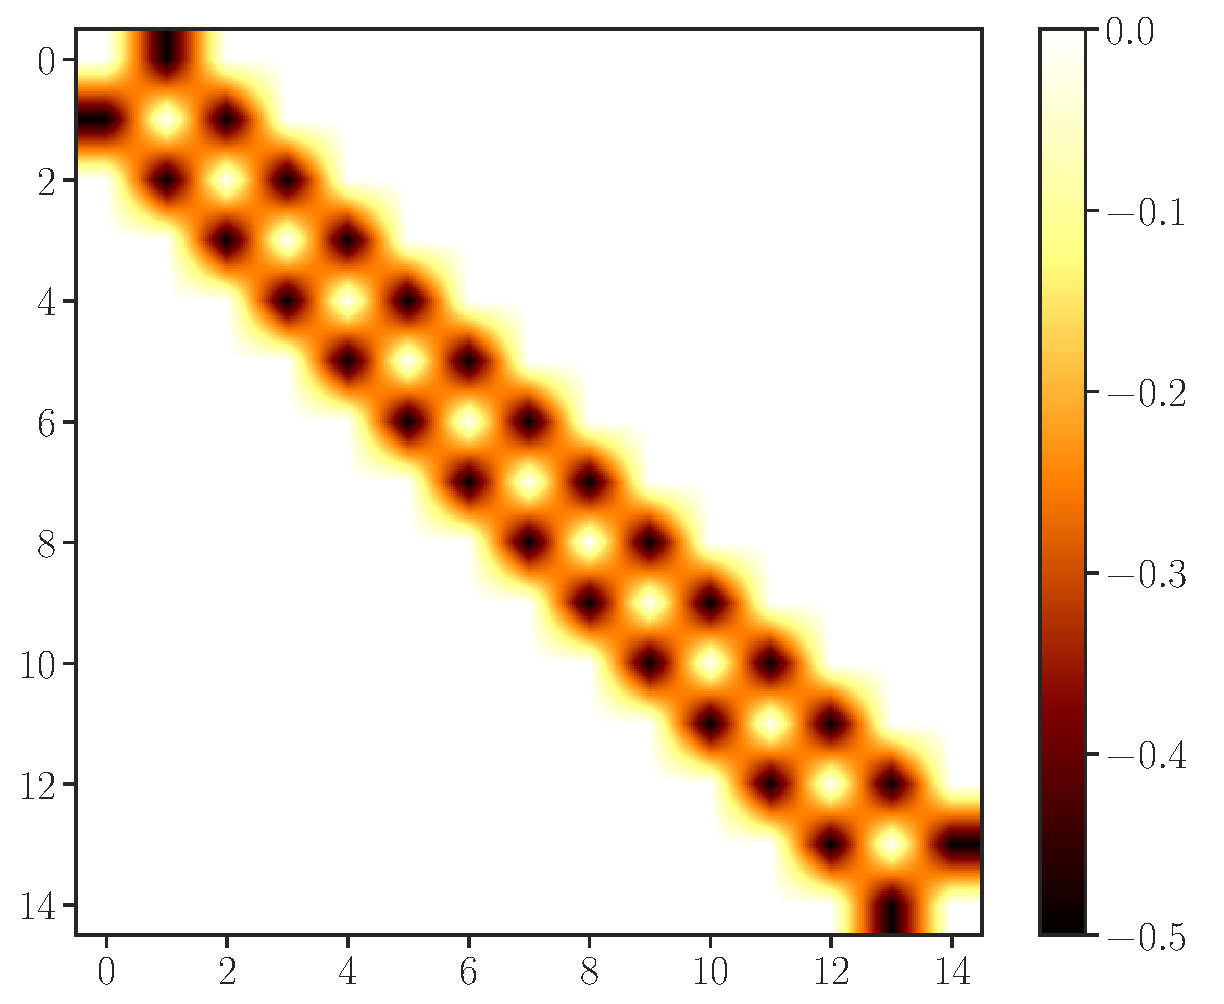
\includegraphics[width=\textwidth]{ColorMapMatrices_OBC}
			\caption{}
		\end{subfigure}
		\begin{subfigure}[b]{0.31\textwidth}
			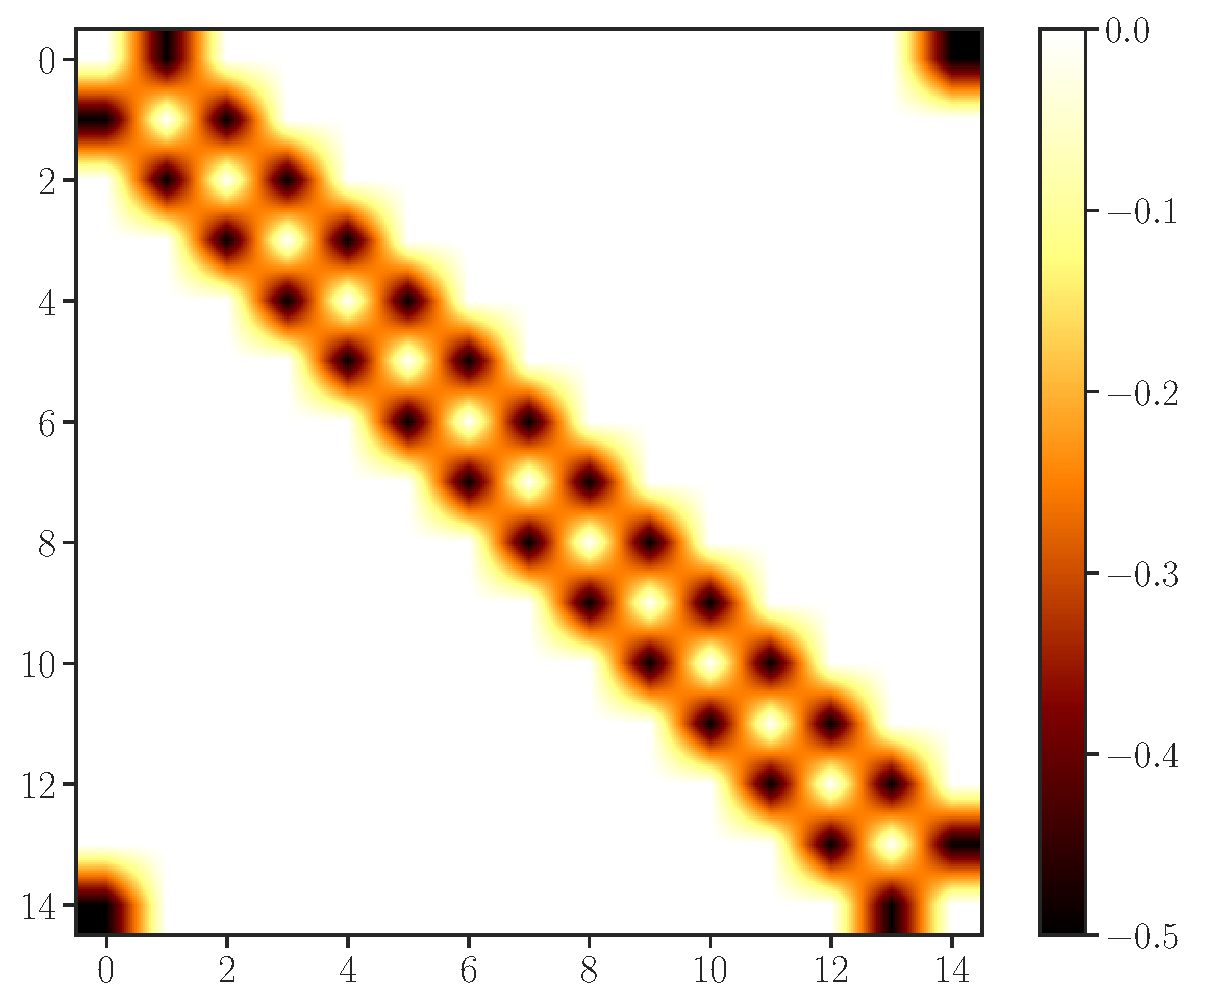
\includegraphics[width=\textwidth]{ColorMapMatrices_PBC}
			\caption{}
		\end{subfigure}
		\begin{subfigure}[b]{0.31\textwidth}
			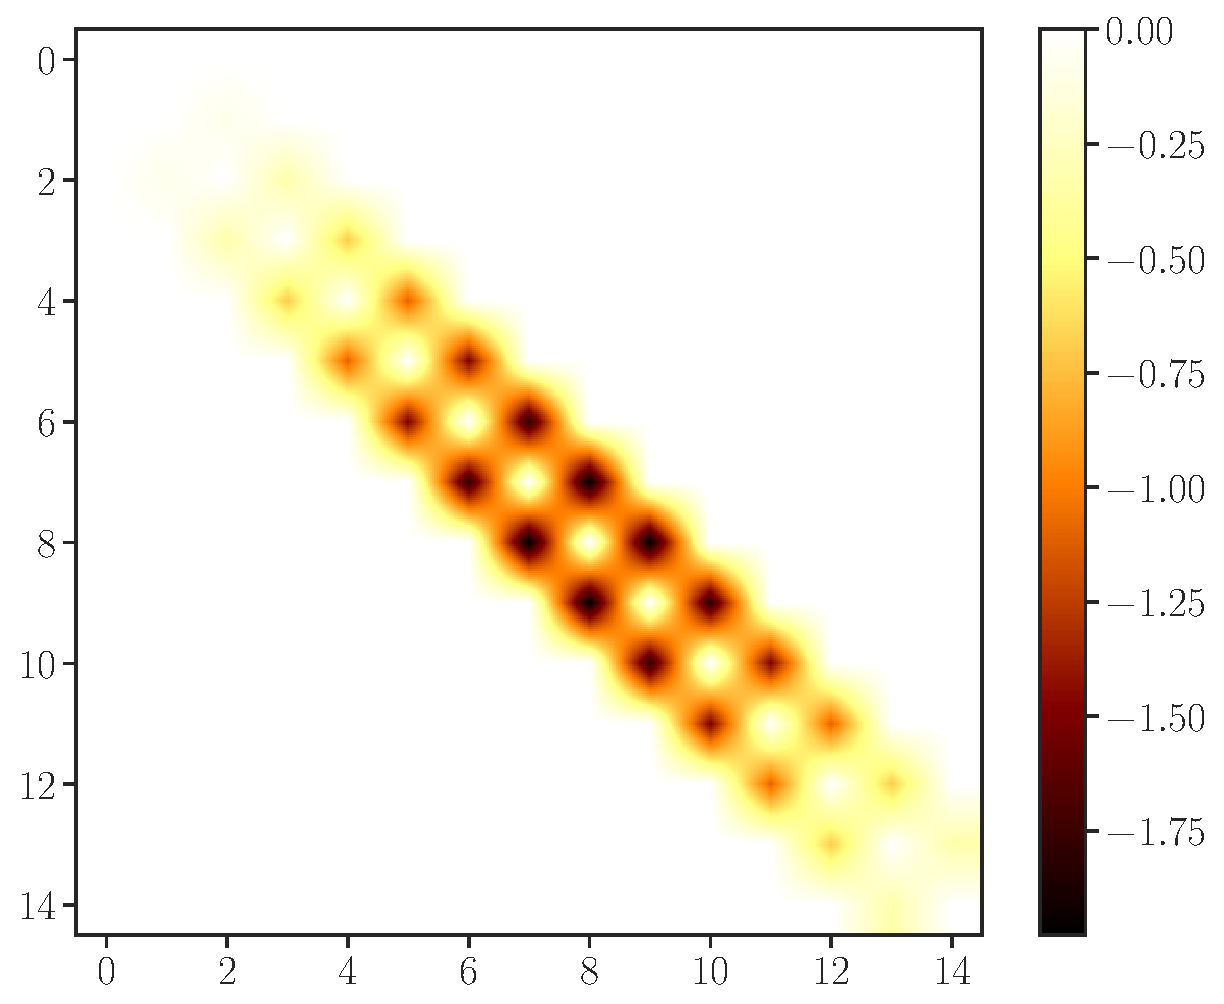
\includegraphics[width = \textwidth]{ColorMapMatrix_SSD}	
			\caption{}
		\end{subfigure}
		\caption{Structure of the tight-binding Hamiltonian for $L = 15$ and (a) open-boundary conditions (b) periodic-boundary conditions (c) sine-squared deformed.}
		\label{fig:matrix_representation_Hamiltonian}
\end{figure}
In all cases, we obtain a bi-diagonal matrix\footnote{If the diagonal elements $E_j$ are also included, we would have a tridiagonal matrix}. For periodic boundary conditions, we additionally have non-vanishing matrix elements $(L, 1)$ and $(1,L)$ in the upper right and lower left corner of the matrix, resulting from the terms $\mel{0}{\hat{c}_m \hat{c}_L^\dagger \hat{c}_1 \hat{c}_n^\dagger}{0}$ and $\mel{0}{\hat{c}_m \hat{c}_1^\dagger \hat{c}_L \hat{c}_n^\dagger}{0}$. 

\subsection{Ground state}

To diagonalize the matrix $\hat{H}_0$, we consider a change of basis from $\{ \ket{\varphi_m}\}$ to some other single-particle basis set $\{ \ket{\phi_j}\}$. In the second quantized formalism, such a change of basis corresponds to the following transformation operation for the creation and annihilation operators:
	 \begin{equation}
	 	\hat{a}_j = \sum_i \braket{\phi_j}{\varphi_i} \hat{c}_i \qq{and} \hat{a}_j^\dagger =\sum_i \braket{\varphi_i}{\phi_j} \hat{c}_i^\dagger
	 	\label{eq:transformation_operators_2nd}
	 \end{equation}
	 where $\hat{a}_j$ and $\hat{a}_j^\dagger$ are also fermionic operators satisfying the anti-commutation relations
	 If we let $U_{i,j} = \braket{\varphi_i}{\phi_j}$ denote the matrix elements of a unitary transformation, we can compactify \ref{eq:transformation_operators_2nd}, as such:
	 \begin{equation}
	 	\hat{a}_j = \sum_i (U^\dagger)_{ji} \hat{c}_i \qq{and} \hat{a}_j^\dagger = \sum_i (U^\dagger)^*_{ji} \hat{c}_i^\dagger =\sum_{i}  \hat{c}_i^\dagger U_{ij}
	 \end{equation}
	 where we used $U_{ij}^* = (U^\dagger)_{ji}$. Similarly, the inverse transformation:
	 \begin{equation}
	 	\hat{c}_n = \sum_i U_{ni} \hat{a}_i \qq{and} \hat{c}_n^\dagger = \sum_i \hat{a}_i^\dagger U^*_{ni} = \sum_i \hat {a}_i^\dagger (U^\dagger)_{in}
	 	\label{eq:inverse_transformation_operators2nd}
	 \end{equation}
	 can be obtained. Lastly, we aim to show that the transformation matrix is indeed unitary. For this, consider:
	 \begin{align}
	 	\delta_{j,k} &= \braket{\phi_j}{\phi_k} = \sum_i \braket{\phi_j}{\varphi_i}\braket{\varphi_i}{\phi_k} = \sum_i \braket{\varphi_i}{\phi_j}^* \braket{\varphi_i}{\psi_k} \\
	 	&= \sum_i U_{ij}^* U_{ik} = \sum_i (U^\dagger)_{ji} U_{ik} = (U^\dagger U)_{jk} \quad \Rightarrow \quad U^\dagger U = \mathbbm{1}
	 \end{align}
	Any hermitian matrix $A$, such as our Hamiltonians $\hat{H}_0$ and $\hat{H}_1$, can then be diagonalized by the unitary similarity transformation:
	 \begin{equation}
	 	U^\dagger A U = \begin{pmatrix}
	 		\lambda_1 & 0 &\dots & 0 \\
	 		0 & \lambda_2 & \dots & 0 \\
	 		\vdots & \vdots & \ddots & \vdots \\
	 		0 & 0 & \dots & \lambda_n
	 	\end{pmatrix}
	 	\label{eq:unitary_similarity_transformation}
	 \end{equation}
	 where $\lambda_1, \dots \lambda_n$ are the eigenvectors of the hermitian matrix $A$ and the columns of $U$ are spanned by the eigenvectors of the hermitian matrix $A$. 
	 \begin{equation}
	 	\hat{H}_0 = \sum_{i=1}^L E_i^{(0)} \hat{a}_i^\dagger \hat{a}_i = E_i^{(0)} \hat{n}_i 
	 \end{equation}
	 where $\hat{n}_i$ denotes the fermionic occupation number operator at site $i$. In the case of periodic boundary conditions, we recover the unitary transformation to the momentum basis, discussed in section \ref{sec:monentum_space_representation} \cite{Xueda}.
	 
\subsubsection{Correlation function ground state}
Once the diagonalizing unitary transformation \ref{eq:unitary_similarity_transformation} for $\hat{H}_0$ has been found, the ground state $\ket{G}$ for the half-filled fermion chain is:
	 \begin{equation}
	 	\ket{\psi(0)} =\ket{G} = \prod_{i=1}^{L/2} \hat{a}_i^\dagger \ket{0}
	 \end{equation}
Consequently, the resulting two-point (one-particle) correlation function is given by:
	\begin{equation}
		\mel{G}{\hat{c}_m^\dagger \hat{c}_n}{G} = \sum_{i \in \text{occ}} U_{ni} (U^\dagger)_{im}
	\end{equation}
	as can readily be verified by inserting the transformations \ref{eq:inverse_transformation_operators2nd} and using the fermionic anti-commutation rules.
	
	 
%	\subsection{Electrons filled on the left hand side of the chain}
%	
%	It can be shown that in this case the correlation matrix will take the form
%	\begin{equation}
%		\mel{H}{\hat{c}_n^\dagger \hat{c}_m}{H} = \sum_{j=1}^{L/2} (\mathcal{W} U^\dagger)_{nj} (U\mathcal{W}^\dagger)_{jm}
%	\end{equation}
%	where $\ket{H}$ corresponds to the state with electrons filled from the left hand side of the chain
%	\begin{equation}
%		\ket{H} = \sum_{j=1}^{L/2} \hat{c}_j^\dagger \ket{0}
%	\end{equation}
%	

\subsection{Single quench}

Next, we aim to find the equal-time two-point correlation function for a single quench:
	\begin{equation}
	\mathcal{C}_{m,n} = \mel{\psi(t)}{\hat{c}_m^\dagger \hat{c}_n}{\psi(t)}	
	\end{equation}
where $\ket{\psi(t)}$ here corresponds to the time evolved ground state $\ket{G}$ by $\hat{H}_1$. Since $\hat{H}_\text{SSD}$ is time-independent, the time evolution of a state in the Schrödinger picture is given by applying the unitary evolution operator $\hat{U} = \exp(i\hat{H}_\text{1} t)$ on the ground state $\ket{\psi(t=0)} = \ket{G}$:
	\begin{equation}
		\ket{\psi(t)} = \exp(-i \hat{H}_1 t) \ket{G}
	\end{equation}
Instead of working in the Schrödinger picture, we will work in the Heisenberg picture and consider time-independent states:
	\begin{equation}
		\mel{\psi(t)}{\hat{c}_m^\dagger \hat{c}_n}{\psi(t)} = \mel{G}{e^{i \hat{H}_1 t} \hat{c}_m^\dagger \hat{c}_n e^{-i \hat{H}_1 t}}{G} = \mel{G}{e^{i\hat{H}_1 t} \hat{c}_m^\dagger e^{-i \hat{H}_1 t} e^{i \hat{H}_1 t} \hat{c}_n e^{-i\hat{H}_1 t}}{G}
		\label{eq:Correlation_Matrix_singlequench}
	\end{equation}
	Where in the second equality we inserted the expression $\hat{U}^\dagger \hat{U} = \exp(i \hat{H}_1 t)\exp(-i \hat{H}_1 t) = \mathbbm{1}$. Our goal will be to simply the two expressions:
	\begin{equation}
		\bra{G} e^{i\hat{H}_1 t} \hat{c}_m^\dagger e^{-i \hat{H}_1 t} \qq{and}  e^{i \hat{H}_1 t} \hat{c}_n e^{-i\hat{H}_1 t}\ket{G}
	\end{equation}
	such that the two-point correlation function \ref{eq:Correlation_Matrix_singlequench} for a single-quench only depends on the unitary transformation that diagonalizes the Hamiltonians $\hat{H}_0$ and $\hat{H}_1$. \\
	
	 We have previously established that the unitary transformation $U$ diagonalizes $\hat{H}_0$. Similarly, another unitary transformation $V$ can be introduced which diagonalizes the sine-squared Hamiltonian $\hat{H}_1$ and results in the following basis change for our operators \cite{Xueda}:
	\begin{equation}
		\hat{b}_j = \sum_i (V^\dagger)_{ji} \hat{c}_i \qq{and} \hat{b}_j^\dagger = \sum_i (V^\dagger)^*_{ji} \hat{c}_i^\dagger =\sum_i \hat{c}_i^\dagger V_{ij}
	\end{equation}
	such that:
	\begin{equation}
		\hat{H}_1 = \sum_i E_i^{(1)} \hat{b}_i^\dagger \hat{b}_i
	\end{equation}
	and:
	\begin{equation}
		\hat{c}_n = \sum_j V_{nj } \hat{b}_j \qq{and} \hat{c}_n^\dagger = \sum_j (V^\dagger)^*_{nj} \hat{b}_j^\dagger = \sum_j \hat{b}_j (V^\dagger)_{jn}
	\end{equation}
	The operators $\hat{b}_j$ and $\hat{b}_j^\dagger$ can analogously be written in terms of our creation and annihilation operators $\hat{a}_i$ and $\hat{a}_i^\dagger$:
	\begin{align}
		\hat{b}_j &= \sum_i (V^\dagger)_{ji} \hat{c}_i = \sum_i (V^\dagger)_{ji} \sum_k U_{ik} \hat{a}_k = \sum_k (V^\dagger U)_{jk} \hat{a}_k \\
		\hat{b}_j^\dagger &= \sum_i  \hat{c}_i^\dagger V_{ij} = \sum_i \sum_k \hat{a}_k^\dagger (U^\dagger)_{ki} V_{ij} = \sum_k \hat{a}_k (U^\dagger V)_{kj}
	\end{align}
	If we define another Matrix as $W = V^\dagger U$ such that $W^\dagger = U^\dagger V$, we obtain the expression:
	\begin{equation}
		\hat{b}_j = \sum_k W_{jk} \hat{a}_k \qq{and} \hat{b}_j^\dagger = \sum_k \hat{a}_k^\dagger (W^\dagger)_{kj}
		\label{eq:expression_b_j}
	\end{equation}
	It follows that:
	\begin{align}
		e^{i \hat{H}_1 t} \hat{c}_n e^{-i \hat{H}_1 t} \ket{G} &=  e^{i \hat{H}_1 t} \sum_j V_{nj} \hat{b}_j e^{-i \hat{H}_1 t}\ket{G} 
	\end{align}
	Using the fact that $e^{i \hat{H}_1 t} \hat{b}_j e^{-i \hat{H}_1 t} = e^{-i E_j^{(1)} t} \hat{b}_j$ and using the expression $\hat{b}_j$ from \ref{eq:expression_b_j}, we get:
	\begin{align}
		\sum_j V_{nj} e^{i \hat{H}_1 t} \hat{b}_j e^{-i\hat{H}_1 t} = \sum_j V_{nj} e^{-i E_j^{(1)}t} \hat{b}_j = \sum_j V_{nj} e^{-i E_j^{(1)} t} \sum_j W_{jk} \hat{a}_k = \sum_j V_{nj} \sum_k W_{jk}^{(t), 1} \hat{a}_k
	\end{align}
	where we additionally defined:
	\begin{equation}
		W_{jk}^{(t),1} = e^{-i E_j^{(1)}} W_{jk}
	\end{equation}
	meaning we have:
	\begin{equation}
		e^{i \hat{H}_1 t} \hat{c}_n  e^{-i \hat{H}_1 t} \ket{G} = \sum_k [ V\cdot W^{(t), 1}]_{nk} \hat{a}_k
		\label{eq:expression_left_Evolution}
	\end{equation}
	Analogously we can show that:
	\begin{equation}
		\bra{G} e^{i \hat{H}_1 t} \hat{c}_m^\dagger e^{-i \hat{H}_1 t} = \sum_{k'}\bra{G} \hat{a}_{k'}^\dagger [V \cdot W^{(t), 1} ]^\dagger_{k',m}
	\end{equation}
	We note that this is simply the complex conjugate expression of \ref{eq:expression_left_Evolution}. Consequently, for the two-point correlation function we obtain:
	\begin{equation}
	\begin{split}
	\mel{G}{e^{i \hat{H}_1 t} \hat{c}_m^\dagger e^{-i\hat{H}_1 t} e^{-i \hat{H}_1 t} \hat{c}_n e^{-i \hat{H}_1 t}}{G} &= \mel {G}{\sum_{k'}\hat{a}_{k'}^\dagger [ V \cdot W^{(t),1}]_{k',m}^\dagger \sum_k [V \cdot W^{(t),1 } ]_{nk} \hat{a}_k}{G}\\
	&= \sum_{k \in \text{occ}} [ V \cdot W^{(t),1} ]_{nk} \cdot [V\cdot W^{(t),1} ]_{km}^\dagger
	\end{split}
	\end{equation}
	where in the second step, we used that the correlation matrix vanishes if $k' \neq k$ and $\mel{G}{\hat{a}_k^\dagger \hat{a}_k}{G} = 1$ for all occupied $k$'s in the ground state \cite{Xueda}.
	
	\subsection{Double quench}
	Moving on one step, we wish to obtain the correlation matrix for a double quench (full cycle) $T = T_0 + T_1$:
\begin{equation}
	\mathcal{C}_{m,n} = \mel{\psi(T)}{\hat{c}_m^\dagger \hat{c}_n}{\psi(T)}
\end{equation}
meaning we consider the state:
	\begin{equation}
		\ket{\psi(T)} = e^{-i \hat{H}_0 T_0} e^{-i \hat{H}_1 T_1} \ket{G}
	\end{equation}
	We have to evaluate:
	\begin{equation}
		e^{i\hat{H}_1 T_1}e^{i \hat{H}_0 T_0} \hat{c}_n e^{-i \hat{H}_0 T_0} e^{-i \hat{H}_1 T_1}\ket{G} = \sum_i U_{ni} e^{-i \epsilon_i^0 T_0} \sum_j (W^\dagger)_{ij} e^{-i\epsilon_j^1 T_1}\sum_k W_{jk} \hat{a}_k \ket{G}
	\end{equation}
	We define
	\begin{equation}
		W_{ik}^{(T_0),0} = e^{-i \epsilon_{i}^0 T_0}(W)^\dagger_{ik}
	\end{equation}
	which yields:
	\begin{equation}
		e^{i\hat{H}_1 T_1}e^{i \hat{H}_0 T_0} \hat{c}_n e^{-i \hat{H}_0 T_0} e^{-i \hat{H}_1 T_1}\ket{G} = \sum_{k \in \text{occ}} \left[ U \cdot W^{(T_0),0} \cdot W^{(T_1),1}\right]_{nk} \hat{a}_k \ket{G}
	\end{equation}
	For which we obtain the following correlation function:
	\begin{equation}
		\mel{\psi(T)}{\hat{c}_m^\dagger \hat{c}_n}{\psi(T)} = \sum_{k \in \text{occ}} \left[ U\cdot W^{(T_0),0} \cdot W^{(T_1),1}\right]_{nk} \cdot \left[ U \cdot W^{(T_0),0} \cdot W^{(T_1),1}\right]^\dagger_{km}
	\end{equation}
	\subsection{Generalization to $n$-cycles}
	The generalization to $n$-cycles, can essentially be seen as a product of double quenches. The wave-function after $n$-cycles with $nT = n(T_0 + T_1)$ is given by:
	\begin{equation}
		\ket{\psi(nT)} = e^{-i \hat{H}_0 T_0} e^{-i \hat{H}_1 T_1} \dots e^{-i \hat{H}_0. T_0 } e^{-i \hat{H}_1 T_1} \ket{G}
	\end{equation}
	and it can straightforwardly be obtained that the resulting correlation function is a product of the unitary transformation matrices:
	\begin{equation}
		\mathcal{C}_{m,n} = \mel{\psi(nT)}{\hat{c}_m^\dagger \hat{c}_n }{\psi(nT)} = \sum_{k \in \text{occ}} \mathcal{W}_{nk}  \cdot (\mathcal{W}^\dagger)_{km}
		\label{eq:correlation_matrix_Xueda}
	\end{equation}
	with 
	\begin{equation}
		\mathcal{W} = U \cdot [W^{(T_0),0} \cdot W^{(T_1), 1}]^n = U \cdot [ W^{(T_0),0} \cdot W^{(T_1), 1}] \dots [ W^{(T_0), 0} \cdot W^{(T_1), 1}] 
	\end{equation}
	and therefore implicitly depends on the how many states $k$ in the lattice are occupied \cite{Xueda}.

	
\section{Conformal field theory}
As previously mentioned, the dynamics of the Floquet protocol \ref{eq:Floquet_Hamiltonian1d} can analytically be solved with conformal field theory. It therefore seems appropriate to introduce some of the concepts found in a conformal field theory, starting with what conformality implies. \\

Letting $g_{\mu \nu}$ denote the metric tensor in a space-time of dimension $d$, the conformal group which describes conformal transformations are a subset of invertible mappings (coordinate transformation) $x^\mu \rightarrow \tilde{x}^\mu(x)$ that leave the metric invariant up to a scale change $\Omega(x)$:
\begin{equation}
g_{\mu \nu}(x) \rightarrow g_{\mu \nu}(\tilde{x}) = \Omega(x) g_{\mu \nu}(x)
= g_{\rho \sigma} \pdv{\tilde{x}^\rho}{x^\mu}\pdv{\tilde{x}^\sigma}{x^\nu}
\label{conformal_transformation} 
\end{equation}
and consequently preserve angles between two arbitrary vectors $v$ and $w$. The set of conformal transformation form the so-called conformal group \cite{Ginsparg}. In two-dimensions, an action of the conformal group can be regarded as two independent actions on $z$ and $\bar{z}$. In general, the transformed metric is of course not proportional to the original metric. To study when it is, we consider an infinitesimal transformation $x^\mu \rightarrow \tilde{x}^\rho = x^\rho + \epsilon^\rho(\vec{x}) + \mathcal{O}(\epsilon^2)$. Then:
\begin{equation}
	\pdv{\tilde{x}^\rho}{x^\mu} = \delta_{\mu}^\rho + \partial_\mu \epsilon^\rho \qq{and} \pdv{\tilde{x}^\sigma}{x^\nu} = \delta_{\nu}^\sigma + \partial_\nu \epsilon^\rho .
\end{equation}
Given this we obtain the following equation:
\begin{align}
	\Omega(x)g_{\mu \nu} &= g_{\rho \sigma} \pdv{\tilde{x}^\rho}{x^\mu}\pdv{\tilde{x}^\sigma}{x^\nu} + \mathcal{O}(\epsilon^2) \\
	&=g_{\rho \sigma}(\delta_{\mu}^\rho \delta_{\nu}^\sigma + \delta_{\mu}^\rho \partial_\nu \epsilon^\sigma + \partial_\mu \epsilon^\rho \delta_\nu^\sigma) + \mathcal{O}(\epsilon^2) \\
	&=g_{\mu \nu} + \delta_\nu \epsilon_\mu + \partial_\mu \epsilon_\nu
\end{align}
To now satisfy the requirement of a conformal transformation \ref{conformal_transformation}, i.e scale invariance, we have to fulfill the condition:
\begin{equation}
	\partial_\mu \epsilon_\nu + \partial_\nu \epsilon_\mu = f(\vec{x}) g_{\mu \nu}
\end{equation}
where the resulting factor $f(\vec{x})= \frac{2}{d} \partial_\rho \epsilon_\rho$ is determined by taking the trace on both sides with $g^{\mu \nu}$:
\begin{equation}
		g^{\mu \nu}(\partial_\nu \epsilon_\mu + \partial_\mu \epsilon_\nu) = f(x) g_{\mu \nu} g^{\mu \nu} \;\Rightarrow \;
		2(\partial_\nu \epsilon^\nu) = d \cdot f(x)
\end{equation}
and $d$ is the dimension of the metric tensor. To conclude we therefore obtain the following scale change:
\begin{equation}
	\Omega(x) = 1 + \frac{2}{d} \partial_\nu \epsilon_\nu
\end{equation}
and the resulting equation is
\begin{equation}
	\partial_\nu \epsilon_\mu + \partial_\mu \epsilon_\nu = \frac{2}{d}(\partial \cdot \epsilon) g_{\mu \nu}
	\label{eq:conformal_requirement}
\end{equation}
For $d=1$, any $\epsilon$ satisfies this equation. For our considerations, mainly the case $d=2$ will be relevant \cite{Schellekens,Francesco}.
\section{Conformal group in two-dimensions}
%Consider a point on the plane $(x_0, x_1)$ and a coordinate change $x^\mu \rightarrow z^\mu = \tilde{x}^\mu(x)$. We know that the covariant metric tensor transforms as
%\begin{equation}
%	g^{\mu \nu} \rightarrow \tilde{g}^{\mu \nu} = \left( \pdv{\tilde{x}^\mu}{x^\alpha}\right) \left( \pdv{z}\right)
%\end{equation}
To simply things, we will mainly be working in Euclidean space, where the metric is defined to be $g_{\mu \nu} = \delta_{\mu\nu}$. In two dimensions the so-called conformal Killing equation \ref{eq:conformal_requirement} reduces to:
\begin{equation}
	\pdv{\epsilon_0}{x_0} = -\pdv{\epsilon_0}{x^1} \qq{and} \pdv{\epsilon_0}{x^0} = \pdv{\epsilon_1}{x^1}
	\label{eq:Cauchy-Riemann}
\end{equation}
Identifying $\epsilon_0$ with the real part of a complex function and $\epsilon_1$ the imaginary part, we notice that we recovered the Cauchy-Riemann equations for holomorphic functions and anti-holormorphic functions. It therefore makes sense to work with complex coordinates $z$ and $\bar{z}$:
\begin{align}
	z = x^0 + ix^1 \qq{and} \bar{z} = x^0 - ix^1 
\end{align}
where 
\begin{equation}
	x^0 = \frac{1}{2}(z + \bar{z}),\quad x^1 = \frac{1}{2i}(z - \bar{z}), \quad \partial_z = \frac{1}{2}(\partial_0 - \partial_1). \quad \partial_{\bar{z}} = \frac{1}{2}(\partial_0 + i\partial_1)
\end{equation}
for which we obtain $\epsilon(z) = \epsilon^0 + i\epsilon^1$ and $\bar{\epsilon}(\bar{z}) = \epsilon^1 - i\epsilon^2$. Since naturally two independent algebras arise when considering the algebra of the conformal transformation generators, we can regard $z$ and $\bar{z}$ as independent coordinates \cite{Schellekens}. This corresponds to the original coordinates $(x_1,x_2) \in \mathbb{R}^2$ to be taken as $(x_1, x_2) \in \mathbb{C}^2$ and then transforming them to $z, \bar{z}$ respectively. It should therefore be emphasized that $\bar{z}$ is a distinct complex coordinate and not simply the complex conjugate of $z$. At some point $\bar{z}$ is then however to be identified with the complex conjugate $z^*$ of $z$ again. It follows that going to complex variables, the equation \ref{eq:Cauchy-Riemann} further reduces to:
\begin{equation}
	\partial_z \epsilon(z, \bar{z}) = 0 \qq{and} \partial_z \bar{\epsilon}(z, \bar{z}) =0
\end{equation}
and analogously for the derivative with respect to $\bar{z}$. The general solution is that $\epsilon$ is an arbitrary function of $z$ and does not depend on $\bar{z}$ and $\bar{\epsilon}$ is an arbitrary function of $\bar{z}$, meaning a two-dimensional conformal transformation coincides with the analytic coordinate transformations:
\begin{equation}
	z \rightarrow f(z), \quad \bar{z} \rightarrow \bar{f}(\bar{z})
\end{equation}
where $f(z)$ is an arbitrary function of $z$. Expressed alternatively, a holomorphic function $f(z) = z + \epsilon(z)$ gives rise to an infinitesimal two-dimensional conformal transformation $z \mapsto f(z)$. \cite{Francesco}\cite{Schellekens}


\subsection{Fields}
Fields only depending on $z$, i.e $\phi(z)$ are called chiral fields and fields $\phi(\bar{z})$ only depending on $\bar{z}$ are called anti-chiral fields. It is also common to refer to them as holomorphic and anti-holomorphic, respectively. The conformal dimensions $(h, \bar{h})$\footnote{the bar here does not mean complex conjugation. Both numbers are real. It simply serves simply to distinguish the two quantities} are obtained from $\phi(z,\bar{z})$ with the scaling transformation $z \rightarrow \lambda z$:
\begin{equation}
	\phi(z, \bar{z}) \mapsto \tilde{\phi}(z,\bar{z}) = \lambda^h \bar{\lambda}^{\bar{h}} \phi(\lambda z, \bar{\lambda}\bar{z})
\end{equation}
If a field, under conformal transformation $z \rightarrow f(z)$, changes such that:
\begin{equation}
	\phi(z,\bar{z}) \rightarrow \tilde{\phi}(z, \bar{z}) =\left(\pdv{f}{z}\right)^h \left(\pdv{\bar{f}}{\bar{z}}\right)^{\bar{h}}\phi(f(z), \bar{f}(\bar{z}))
	\label{eq:conformal_transformation2d}
\end{equation}
it is referred to as a primary field of conformal dimension $(h, \bar{h})$. This is equivalent to the statement that $\phi(z, \bar{z}) \dd z^h \dd \bar{z}^{\bar{h}}$ is invariant. If this statement only holds for $f \in$ SL$(2,\mathbb{C})/\mathbb{Z}^2$, i.e only for global conformal transformations\footnote{A section on the Witt algebra and global versus local transformation, can be found in the Appendix}, then $\phi$ is called a quasi-primary field \cite{Blumenhagen}.
\section{Floquet conformal field theory}
\label{sec:Floquet_Conformal_Field_Theory}
In this section we will briefly give an overview of some of the results found in the Floquet Conformal Theory \cite{Xueda}\cite{Lapierre}\cite{Andersen} which will give us a theoretical analytically solvable method for obtaining many of the quantities we wish to consider. To describe the Floquet system with the help of conformal field theory, it is convenient to instead work with the energy-momentum tensor. In such framework, our Floquet system can be described by:
	\begin{equation}
	\hat{H}(t) = 
		\begin{dcases}
		\hat{H}_\text{SSD} = \int_0^L \dd x \, T_{00}(x)\quad &0<t< T_1 \\
		\hat{H}_0 = 2\int_0^L \dd x \, \sin^2\left(\frac{\pi x}{L} \right) T_{00}(x) &T_1 < t < T_1 + T_0
		\end{dcases}
	\end{equation}
 Let $\ket{\psi(nT)}$ be the stroboscopic time evolved Floquet state after $n$ cycles. Most of the quantities we aim to study can be obtained by evaluating the two-point correlation function $G(x_2,T,x_2,0)= \mel{\psi(nT)}{\mathcal{O}_1(x_1) \mathcal{O}_2(x_2)}{\psi(nT)}$ of two local operators $\mathcal{O}(x_1)$ and $\mathcal{O}_2(x_2)$. Introducing Euclidean coordinates $\omega = \tau + ix$ and imaginary time, the two local operators we wish to consider are the fields $\phi(\omega_1, \bar{\omega}_1)$ and $\phi(\omega_0, \bar{\omega_0})$. For a 1-cycle drive, the resulting two-point correlation function is then given by:
 \begin{equation}
 	G(x, \tau,x_0, 0) = \expval{e^{\tau_1 \hat{H}_\text{SSD}} e^{\tau_0 \hat{H}_0} \phi(\omega_1, \bar{\omega_1}) e^{-\tau_0 \hat{H}_0} e^{-\tau_1 \hat{H}_\text{SSD}}\phi(\omega_0, \bar{\omega_0})}
 \end{equation}
where we have and $\tau = \tau_0 + \tau_1$. Next we map to the complex plane with the conformal mapping $z = \exp(2\pi \omega/L)$. Since we assumed that $\phi$ is a primary field, according to equation \ref{eq:conformal_transformation2d} we expect the two-point function to transform as follows:
\begin{equation}
	G(x, \tau;x_0, 0) = \left(\pdv{z_1}{\omega_1}\right)^h \left(\pdv{\bar{z}_1}{\bar{\omega}_1} \right)^{\bar{h}}\expval{e^{\tau_1 \hat{H}_\text{SSD}} e^{\tau_0 \hat{H}_0} \phi(z_1, \bar{z_1}) e^{-\tau_0 \hat{H}_0} e^{-\tau_1 \hat{H}_\text{SSD}}\phi(z_0, \bar{z_0})}
\end{equation}
where one can readily verify that:
\begin{equation}
	\left(\pdv{z_1}{\omega_1}\right)^h \left(\pdv{\bar{z}_1}{\bar{\omega}_1} \right)^{\bar{h}} = \left(\frac{2\pi}{L}\right)^{4h}
\end{equation}
This is equivalent to evaluating the evolution of the operator $\mathcal{O}(nT) = F^{-n} \mathcal{O}_1(x_1) \mathcal{O}_2(x_2) F^n$ and applying it to the ground state $\ket{\psi_0}$ of $\hat{H}_0$. Generally such operator evolution does not have a closed form solution \cite{Lapierre}. It turns out however, that for the Floquet drive with the SSD Hamiltonian as a deformation, the time evolution of the operator product $\mathcal{O}_1(x_1) \mathcal{O}_2(x_2)$ for a one-cycle time translation is equivalent to a Möbius transformation \footnote{which is inherently conformal (angle preserving).} for each point in $\mathbb{C}$:
\begin{equation}
	\tilde{z_1} = f(z) = \frac{az + b}{cz + d} \qq{with} a,b,c,d \in \mathbb{C}, ad - bc \neq 0
\end{equation}
with the parameters:
\begin{align*}
a &= \left( 1 + \frac{\pi \tau_1}{L}\right)\exp( \frac{\pi \tau_0}{L}), &  b &= - \frac{\pi \tau_1}{L} \exp(- \frac{\pi \tau_0}{L}) \\
c & = \frac{\pi \tau_1}{L}\exp(\frac{\pi \tau_0}{L}), & d &= \left( 1 - \frac{\pi \tau_1}{L} \right)\exp(- \frac{\pi \tau_0}{L})
\end{align*}
where $\tau_0 = i T_0$ and $\tau_1 = iT_1$ represent the imaginary time periods. The two-point function at different times for a 1-cycle drive is then more explicitly determined by:
\begin{equation}
	\expval{e^{\tau_1 \hat{H}_{\text{SSD}}} e^{\tau_0 \hat{H}_0} \phi(\omega_1, \bar{\omega_1}) e^{-\tau \hat{H}_0} e^{-\tau_1 \hat{H}_{\text{SSD}}} \phi(\omega_0, \bar{\omega}_0)} = \left(\frac{2\pi}{L}\right)^{4h} \left(\pdv{\tilde{z}_1}{z_1}\right)^h \left(\pdv{\tilde{\bar{z_1}}}{\bar{z}_1}\right)^{\bar{h}} \expval{\phi(\tilde{z}_1, \tilde{\bar{z}}_1) \phi(z_0, \bar{z}_0)}
\end{equation}



and we obtain the following expression for the operator evolution:
\begin{equation}
	F^{-1} \mathcal{O}(z, \bar{z}) F^1 = \left( \pdv{z_1}{z} \right)^h \left( \pdv{\bar{z}_1}{\bar{z}} \right)^{\bar{h}} \mathcal{O}(z_1, \bar{z}_1)
\end{equation}

%\begin{equation}
%	G(x, T, x_0, 0) = e^{H_1 \tau_1}e^{H_0 \tau_0} \mathcal{O}(\omega, \bar{\omega})e^{-H_0 \tau_0} e^{-H_1 \tau_1} = \left(\pdv{z}{w}\right)^h \left( \pdv{\bar{z}}{\bar{w}}\right)^{\bar{h}} \left(
%\end{equation}

%
%and therefore
%\begin{equation}
%	\mel{\psi_0}{\mathcal{O}(x,t)\mathcal{O}{x_0,0}
%\end{equation}
Obtaining the $n$-cycle Floquet time evolution, can be simply be seen as a the following composition of the initial Möbius transformation:
\begin{equation}
	\tilde{z}_n = f^n(z) = \frac{Az + B}{Cz + D}
	\label{Möbius_Transformation}
\end{equation}
The two-point correlation function for stroboscopic times after $n$ cycles is best obtained by expanding the $n$-cycle Möbius transformation by writing the 1-cycle Möbius transformation in its normal form, which centers around finding the fixed points $f(\gamma) = \gamma$. For a single-cycle, this yields the following quadratic condition:
\begin{equation}
	c\gamma^2 - (a-d)\gamma - b = 0
\end{equation}
which has at most two fixed points, with the exception of the identity mapping $z \mapsto f(z) = z$. Denoting the two fixed point of the Möbius transformation as $\gamma_{1}$ and $\gamma_2$, the above equation gives us the two roots:
\begin{equation}
	\gamma_{1} = \frac{a - d - \sqrt{(a-d)^2 + 4bc}}{2c}, \quad \gamma_2 = \frac{a - d + \sqrt{(a-d)^2 + 4bc}}{2c}
\end{equation}
To include the fact that we are considering $n$-cycles, we introduce the rotation $\eta$ (also referred to as multiplier) relative to the fixed points:
\begin{equation}
	\eta = \frac{c\gamma_2 + d}{c \gamma_1 + d} = \frac{a + d + \sqrt{(a-d)^2 + 4bc}}{a + d - \sqrt{(a-d)^2 + 4bc}}
	\label{eq:multiplier}
\end{equation}
The normal form for a one-cycle evolution simply amounts to finding the points $z_1$ satisfying:
\begin{equation}
	\frac{\tilde{z}_1 - \gamma_1}{\tilde{z}_1 - \gamma_2} = \eta \frac{z - \gamma_1}{z - \gamma_2}
\end{equation}
and for $n$-cycles:
\begin{equation}
	\frac{\tilde{z}_n - \gamma_1}{\tilde{z}_n - \gamma_2} = \eta^n \frac{z - \gamma_1}{z - \gamma_2}
\end{equation}
This shows that the characteristics of the entire stroboscopic time evolution is encoded in the multiplier $\eta$. We note that since $a = \bar{d}$ (where here the hat does denote complex conjugation) the first term $a - d$ in the multiplier $\eta$ in equation (\ref{eq:multiplier}) is real. Without having explicitly found the form of the correlation function, the stroboscopic time evolution can already be classified, according to the sign of term inside the square root of $\eta$ \cite{Andersen}:
\begin{equation}
	\Delta = \frac{1}{4} (a -d)^2 + bc
\end{equation}
\begin{enumerate}
	\item \textbf{Elliptical Class:} In this case the equation $f(\gamma) = \gamma$ has two distinct roots which are conjugate to each other $\gamma_1 = \gamma_2^*$ and the rotation parameter $\eta$ is a pure phase $\abs{\eta}=1$, i.e $\eta \in \mathbb{C}$  which corresponds to an imaginary $\Delta < 0$. The system is periodic, corresponding to the \textit{non-heating phase}.
	\item \textbf{Hyperbolic Class:} The two distinct roots $\gamma_1$ and $\gamma_2$ are real. This corresponds to $\Delta > 0$ since then the square root is also real and consequently $\eta \neq 1$ and $\eta \in \mathbb{R}$. This corresponds to the \textit{heating phase}.
	\item \textbf{Parabolic Class:} The two roots coincide with each other $\gamma = \gamma_1 = \gamma_2$ due to vanishing discriminant $\Delta = 0$. The transformation, which sends the fixed point $\gamma $ to infinity is given by:
	\begin{equation}
		g(z) = \frac{1}{z -\gamma}
	\end{equation}
	If $\gamma = \infty$ is the sole fixed point, then the transformation $gfg^{-1}$ fixes infinity which has to imply that $f(z)$ is a translation, i.e $f(z) = z + b$. This corresponds to the \textit{critical phase}.
\end{enumerate}

Using an analytic continuation $\tau \rightarrow it$ and inserting the explicit expression for our parameters, $\Delta$ is given by:
\begin{equation}
	\Delta = \left( \frac{\pi^2 T_1^2}{L^2} - 1\right)\sin^2\left(\frac{\pi T_0}{L}\right) - \frac{\pi T_1}{L}\sin^2\left( \frac{2\pi T_0}{L}\right)
	\label{eq:Delta}
\end{equation}
and is clearly periodic in $T_0$. The $n$ cycle Möbius transformation can then explicitly be written in terms of the parameters:
\begin{align}
	A &= \gamma_1 - \eta^n \gamma_2, & B &= (\eta^n - 1) \gamma_1 \gamma_2 \\
	C &= 1 - \eta^n, & D &= \gamma_1 \eta^n - \gamma_2
\end{align}

\subsection{Conformal transformations of the Energy-Momentum Tensor}
In general, the energy-momentum tensor is not a primary field since it has a non-vanishing central charge $c$ \cite{Ginsparg}. Under a conformal transformation $z \rightarrow f(z)$ the energy-momentum tensor therefore transforms slightly different than a primary field:
\begin{equation}
	\Tilde{T}(z) = \left( \pdv{f}{z}\right)^2 T(f(z)) + \frac{c}{12} S(f(z),z)
\end{equation}
where $S(f(z),z)$ denotes the Schwarzian derivative:
\begin{equation}
	S(f,z) = \frac{1}{(\partial_z f)^2}\left( (\partial_z f) (\partial_z^3 f) - \frac{3}{2}(\partial_z^2 f)^2\right)
\end{equation}
The Schwarzian derivate can be thought of as a tool to measure to what extent a transformation corresponds to a Möbius transformation. We note that we only obtain a Schwarzian derivative if we transform between different geometries, not however, if we transform between Möbius transformations. The first step is to map the strip to the complex plane using the exponential mapping $z = \exp(2\pi \omega/L)$:
\begin{equation}
	\mel{G}{F^{-n} T(\omega) F^{n}}{G} = \left(\pdv{z}{w}\right)^2 \mel{G}{F^{-n} T(z) F^{n}}{G} - \left( \frac{2 \pi}{L}\right)^2 \frac{c}{24}
\end{equation}
Now, we map the complex plane to itself, resulting in the driven möbius coordinates $\tilde{z}_n$. After $n$-cycle driving, the expectation value of the energy-momentum tensor on the strip therefore becomes:
\begin{equation}
	\mel{G}{\hat{F}^{-n} T(\omega) \hat{F}^n}{G} = \left(\pdv{z}{w}\right)^2 \left(\pdv{\tilde{z}_n}{z}\right) \mel{G}{T(\tilde{z}_n)}{G}- \left(\frac{2\pi}{L}\right)^2 \frac{c}{24}
\end{equation}
Lastly, we need to evaluate the expectation value of the energy-momentum tensor $\mel{G}{T(\tilde{z}_n)}{G}$. This is done by performing another conformal transformation to the upper half-plane with $\xi = \sqrt{z} = \exp(\pi \omega /L)$. Since this is not a Möbius transformation this generates a Schwarzian derivative:
\begin{equation}
	\frac{c}{12}S(\xi,z) =  \frac{c}{12} \left( \frac{\xi'''(z)}{\xi'(z)} - \frac{3}{2} \left( \frac{\xi''(z)}{\xi'(z)}\right)^2 \right) = \frac{c}{32z^2}
\end{equation}
meaning we have:
\begin{equation}
	\mel{G}{\hat{F}^{-n} T(\omega) \hat{F}^n}{G} = \left(\pdv{z}{w}\right)^2 \left(\pdv{\tilde{z}_n}{z}\right) \left[ \mel{G}{T(\xi)}{G} + \frac{c}{32{z_n}^2}\right]- \left(\frac{2\pi}{L}\right)^2 \frac{c}{24}
\end{equation}
It turns out that $\mel{G}{T(\xi)}{G}$ is translationally invariant in the horizontal direction and therefore vanishes. Subtracting the initial term obtained from the Schwarzian derivative, we get:
\begin{equation}
	\mel{G}{F^{-n} T(\omega) F^{n}}{G} = \left( \pdv{z}{w} \right)^2 \left(\pdv{\tilde{z}_n}{z}\right)^2 \frac{c}{32\tilde{z}_n^2}
\end{equation}
and the energy density is given by:
\begin{equation}
	\mathcal{E}(x,t) =  \expval{T(x,nT)} + \expval{\bar{T}(x, nT)} = \frac{c}{32}\left[\left( \pdv{z}{w} \right)^2 \left(\pdv{\tilde{z}_n}{z}\right)\frac{1}{\tilde{z}_n^2} + \left(\pdv{\bar{z}}{\bar{\omega}}\right)^2 \left(\pdv{\bar{\tilde{z}}_n}{\bar{z}}\right) \frac{1}{\bar{\tilde{z}}_n^2}  \right]
\end{equation}
After an analytic continuation $\tau_0 \rightarrow iT0, \tau_1 \rightarrow i T_1$, the expectation value of $T$ and $\bar{T}$ can be expressed in terms of the Möbius parameters \ref{Möbius_Transformation}:
%TODO How to get to this equation
\begin{equation}
\begin{split}
	\expval{T(x,t = nT)} = \left( \frac{2\pi}{L}\right)^2 \frac{c}{32}\frac{(AD - BC)^2 z^2}{(Az + B)^2(Cz + D)^2} \\
	\expval{\bar{T}(x, t = nT)} = \left(\frac{2\pi}{L}\right)^2 \frac{c}{32} \frac{(AD - BC)^2 \bar{z}^2}{(A\bar{z} + B)^2 (C\bar{z} + D)^2}
\end{split}
\end{equation}
The total energy is then constructed as follows:
\begin{equation}
	E(t = nT) = \frac{1}{2\pi}\int_{0}^L \dd x \; (\expval{T} + \expval{\bar{T}}) = \frac{2\pi}{L} \frac{c}{16} \frac{AD + BC}{AD - BC}
\end{equation}
As expected, total energy and energy density expect therefore implicitly depend on the parameters $T_0/L$ and $T_1/L$ and $n$ \cite{Lapierre}.
\section{Evolution of energy and energy density}
Equipped with the knowledge of Floquet CFT, we turn to our lattice model again. The aim of this section will be to study the evolution of the total energy $E$ and energy density $\mathcal{E}$. Obtaining the total energy corresponds to forming the expectation value with the time-evolved state $\ket{\psi(nT)}$ and can be written in terms of the previously obtained correlation function (\ref{eq:correlation_matrix_Xueda}) as follows:
\begin{equation}
	E(nT) =\expval*{\hat{H}_0} = \mel{\psi(nT)}{\hat{H}_0}{\psi(nT)} = \sum_{i=1}^{L-1} \mathcal{C}_{i, i+1} + \mathcal{C}_{i+1, i}
	\label{eq:Total_Energy}
\end{equation}
In the preceding section, we established, that the total energy implicitly depends on the driving parameters $T_0/L$ and $T_1/L$. Our goal will be to analyze exactly how the driving parameters influence the total energy of our system. The result for $T_0/L = [0, 2]$ and $T_1/L = [0, 2]$ can be seen in Fig. \ref{fig:Phase_Diagram_Total_Energy}. As expected from Floquet conformal field theory, we observe the formation of two phases; heating in the low-frequency driving regime and non-heating in the high-frequency driving regime, corresponding to the hyperbolic and elliptical class of Möbius transformations respectively. We also note, that the phase diagram is periodic in $T_0/L$ and aperiodic in $T_1/L$\footnote{ This is expected, since $\Delta$ from \ref{eq:Delta} is periodic in $T_0$ and aperiodic in $T_1$}. \\

Furthermore, we observe in Fig. \ref{eq:Evolution_of_total_energy}, that the energy in the heating phase exponentially grows as the number of cycles $n$ is increased and periodically varies in the non-heating phase\footnote{The phase for the non-heating case is dependent on the parameters $T_0$ and $T_1$}. It should be noted that the parameters chosen for the heating phase in Fig. \ref{eq:Evolution_of_total_energy} correspond to a slowly heating system, since the exponential increase only holds in the low-energy limit. Inevitably, as the cycles increase, the total energy starts to plateau \cite{Fan}. \\

\begin{figure}[h]
	\centering
	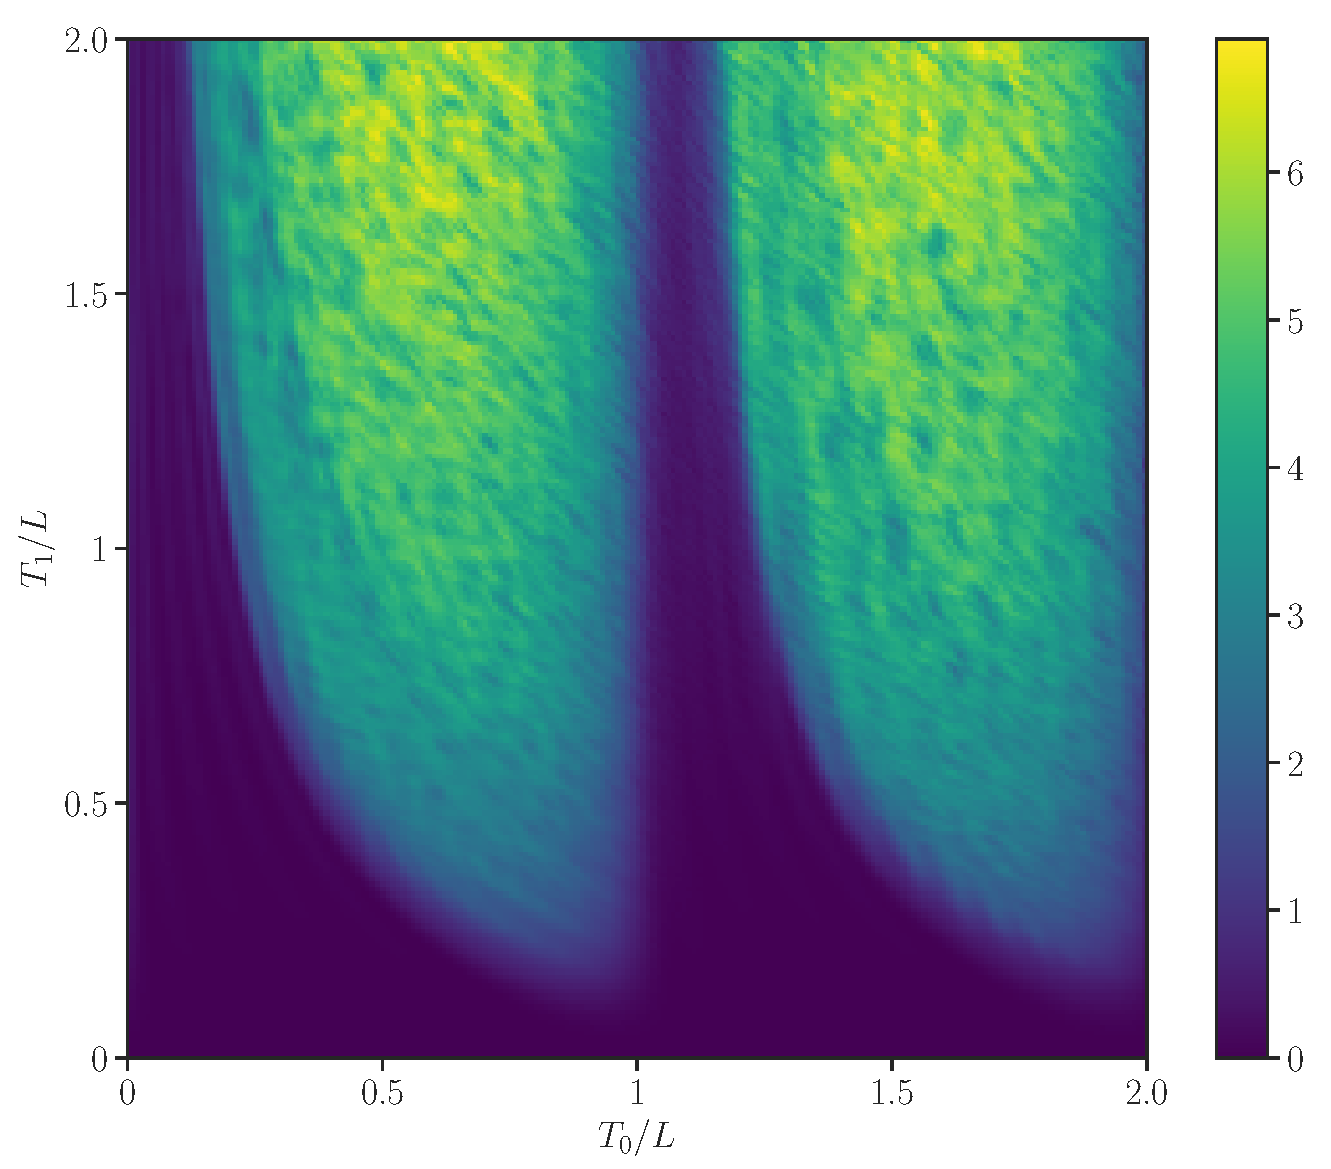
\includegraphics[width=0.8\textwidth]{PhaseDiagram}
	\caption{The Total Energy for a 6-cycle Floquet driven one-dimensional system of $L = 100$ sites as a function of the the two different driving periods $T_0$ and $T_1$.}
	\label{fig:Phase_Diagram_Total_Energy}
\end{figure}
For a quickly heating system in the low-frequency, long-time regime (for example, $T_0/L = 0.5$ and $T_1/L = 1.5$) the total energy quickly converges to its maximum energy value. This is to be expected, as the Hilbert space is finite dimensional (meaning only a finite number of eigenstates and finite energies $E_m$ exist). We can see this limitation analytically by considering that in a finite system, the time-evolved Floquet state can be expanded in terms of energy-eigenfunctions $\ket{u_m}$ as follows; $\ket{\psi(nT)} = \sum_m c_m(nT) \ket{u_m}$. For the total energy after $n$-cycles we therefore have:
\begin{equation}
\begin{split}
	E(nT) &= \mel{\psi(nT)}{\hat{H}_0}{\psi(nT)} \\
	&= \sum_{m,m'} c_m(nT) c_{m'}(nT) \mel{u_{m'}}{\hat{H}_0}{u_m}
\end{split}
\end{equation}

\begin{figure}[h]
\centering
\begin{subfigure}[t]{0.49\textwidth}
	\centering
	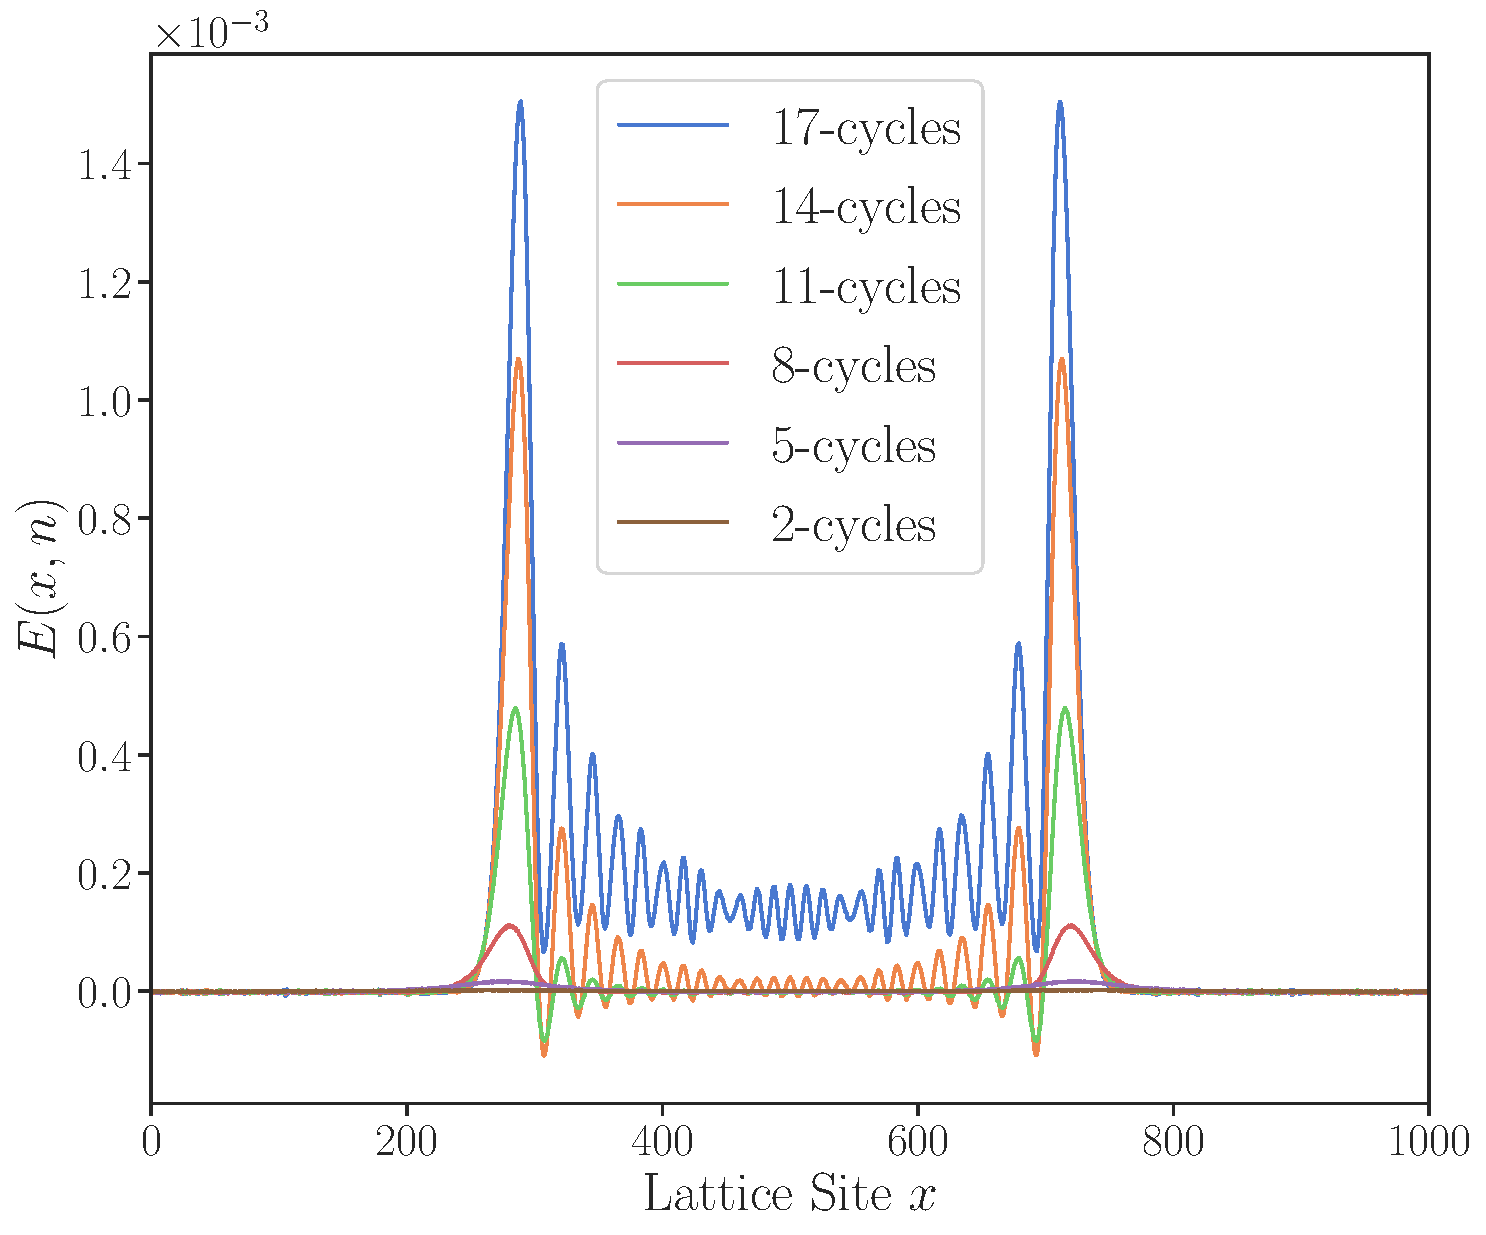
\includegraphics[width =\textwidth]{Energy_Density1}
	\caption{}
	\label{Energy_density_heating}
\end{subfigure}
\begin{subfigure}[t]{0.49\textwidth}
	\centering
	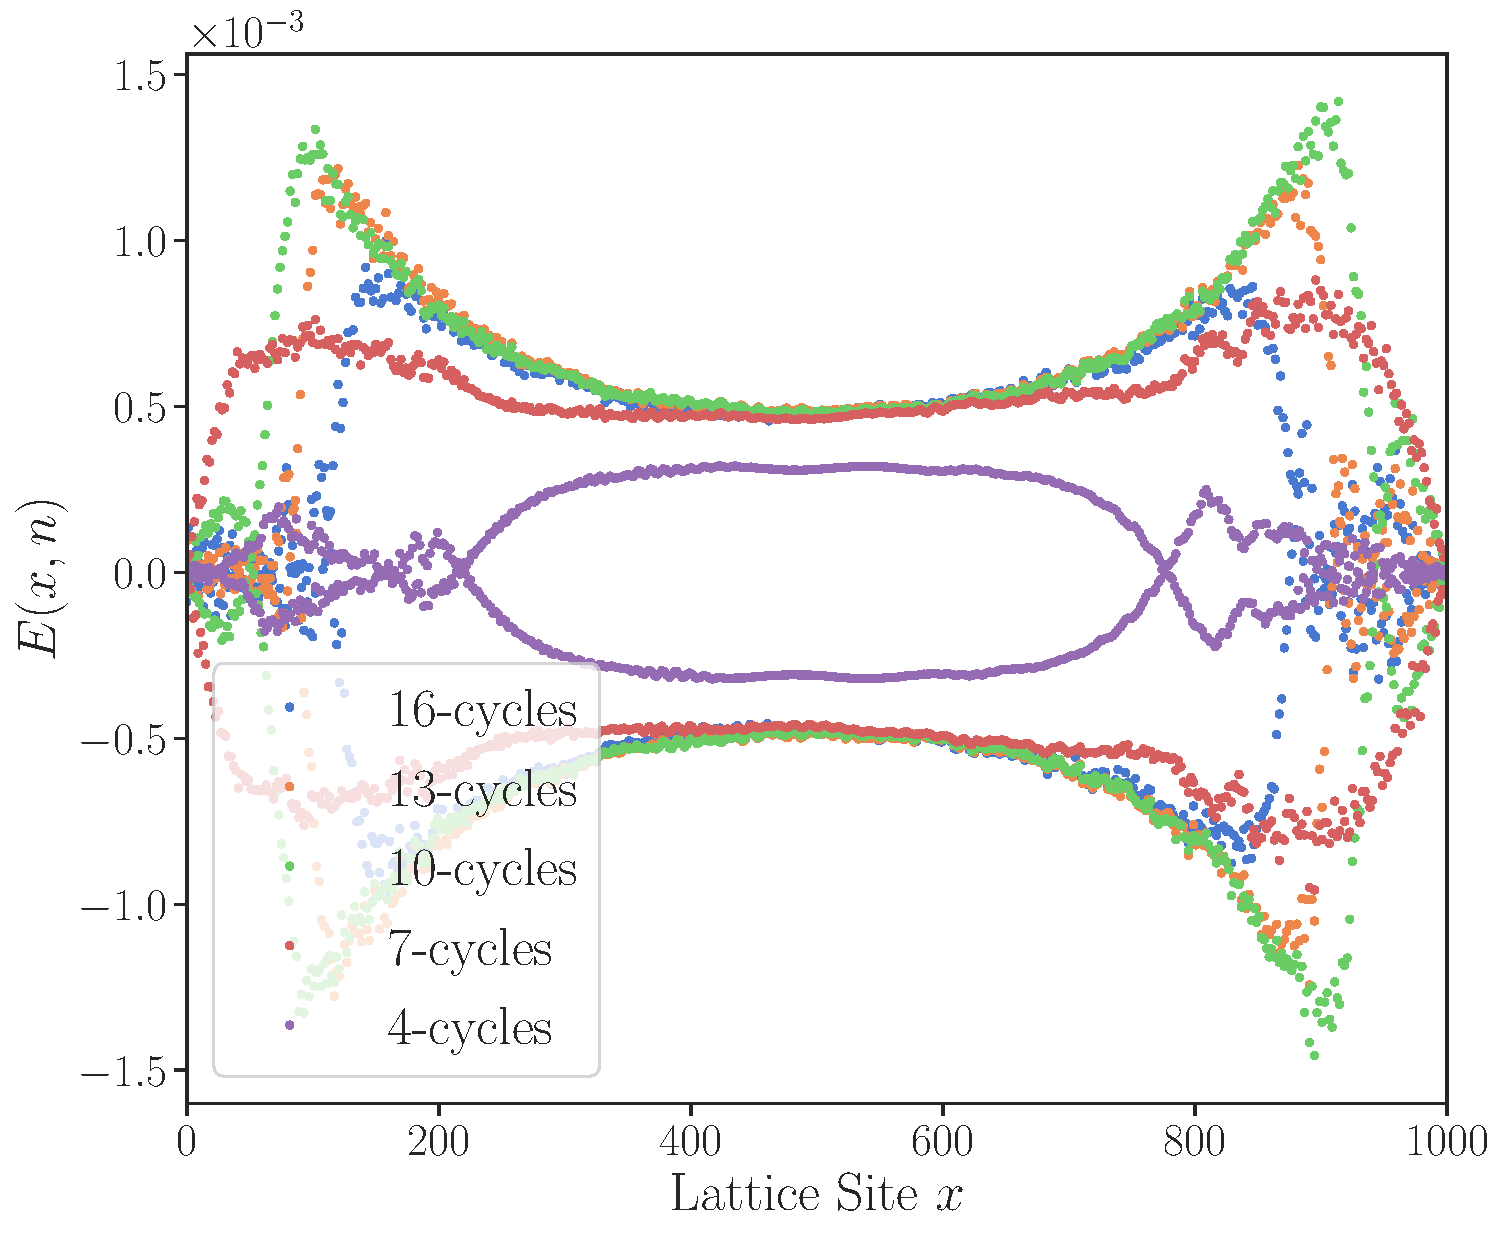
\includegraphics[width =\textwidth]{Energy_Density2}
	\caption{}
	\label{Energy_density_non-heating}
\end{subfigure}
\caption{Energy density for a heating phase (a) $T_0 = 0.95L, T_1 = 0.05L$ and non heating phase (b) $T_0 = 0.2L, T_1 = 0.8L$. The CFT-predicated locations for the chiral peak and anti-chiral peak in the heating phase are $x_{\text{chiral}} = 276$ and $x_{\text{anti-chiral}} = 724$.}
\end{figure}
Using the eigenvalue equation $\hat{H}_0 \ket{u_m} = E_m \ket{u_m}$, we get
\begin{equation}
\begin{split}
	E(nT) &= \sum_{m,m'} c_m(t) c_{m'}(t) E_m \delta_{m,m'} \\
	&= \sum_m \abs{c_m(t)}^2 E_m \qq{with} \sum_m \abs{c_m(t)}^2 = 1
\end{split}
\end{equation}
In this picture, the infinite temperature state therefore simply corresponds to the saturated maximal energy state. \\

To better understand in what manner the heating occurs, we wish to analyze the energy density, which can be regarded as the local component of the total energy \ref{eq:Total_Energy} and is therefore given by:
\begin{equation}
	\mathcal{E}(i,n) = \mathcal{C}_{i, i+1} + \mathcal{C}_{i+1, i}
\end{equation}
The energy density for the heating phase and non-heating phase  in an early-time regime are shown in Fig. \ref{Energy_density_heating} and \ref{Energy_density_non-heating}, respectively. We observe, that in the heating phase, most of the energy accumulates around two peaks, whereas in the non-heating phase the energy keeps oscillating in a patternless manner as the number of cycles increases. As established in section \ref{sec:Floquet_Conformal_Field_Theory}, the Floquet dynamics boils down to classifying conformal mappings according to their fixed points $\gamma_1$ and $\gamma_2$ or the sign inside the square root of the multiplier $\eta$. The location of the energy peaks can then be determined with the unstable fixed point of the Möbius transformation:
	$x_{\text{chiral}} = L\log(\gamma_2)/2\pi$ and $x_{\text{anti-chiral}} = L - L\log(\gamma_2)/2\pi$ \cite{Xueda}. We find, that the anti-chiral and chiral peaks calculated in the Floquet CFT framework are consistent with the accumulation points found in our lattice model.\\

For a late-time regime corresponding to cycles roughly larger than $n = 18$, however, the CFT predictions are not accurate anymore, since more and more excitations other than the chiral and anti-chiral appear. In Fig. \ref{fig:Energy_density-late-regime}, for example, the energy density for a heating phase in the late-time regime can be seen. As expected, we observe smeared out, saturated chiral and anti-chiral peaks\footnote{This is due to the fact that there are only a finite number of degrees of freedom.} and emerging excitations near the center of the system \cite{Fan}.







\begin{figure}
\centering
\begin{subfigure}[t]{0.49\textwidth}
	\centering
	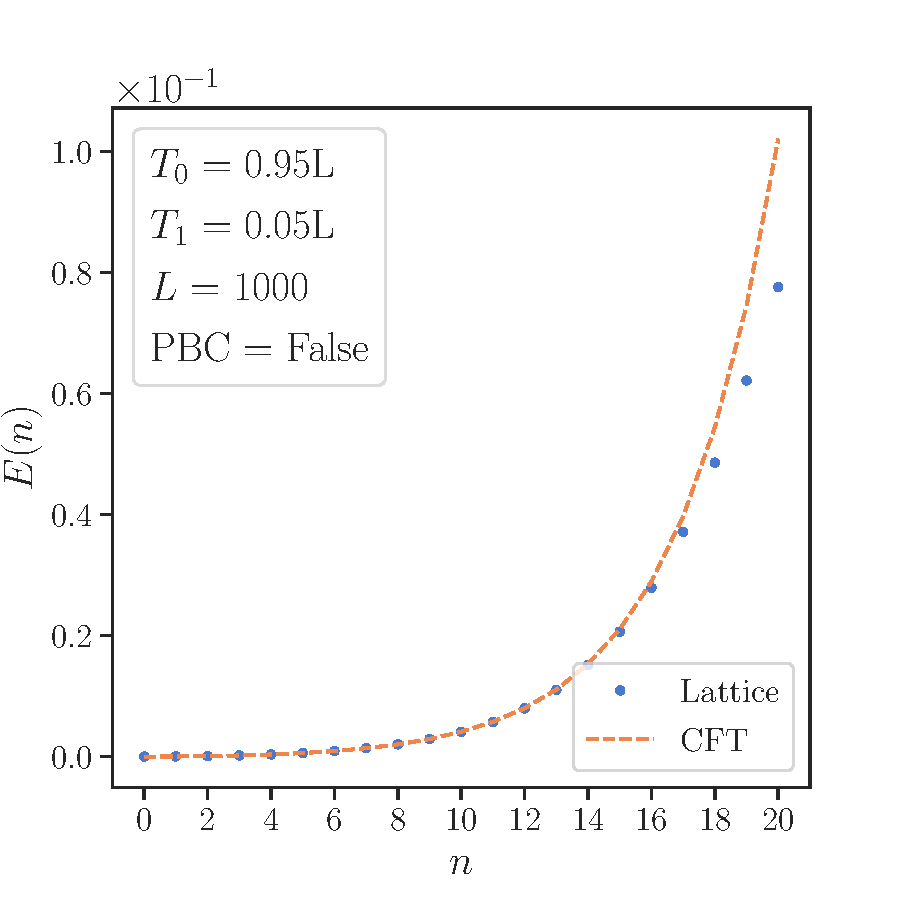
\includegraphics[width =\textwidth]{TotalEnergyHeating}
	\end{subfigure}
\begin{subfigure}[t]{0.49\textwidth}
	\centering
	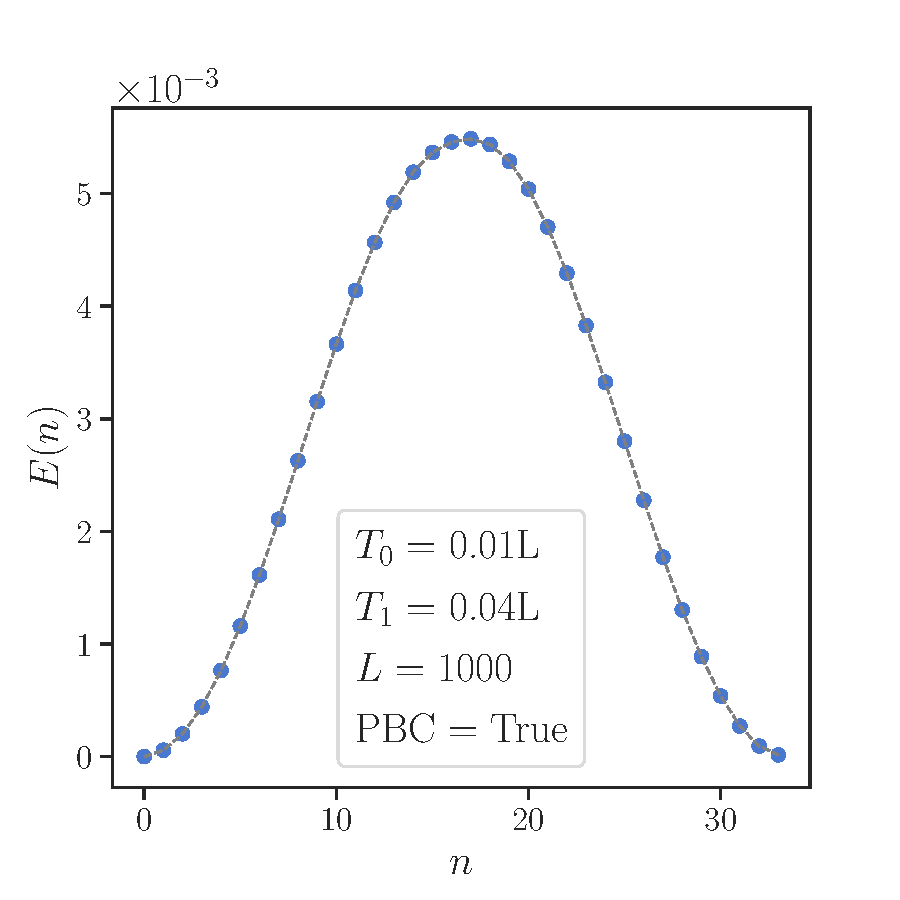
\includegraphics[width =\textwidth]{TotalEnergyNonHeating}
\end{subfigure}
\caption{Evolution of total energy $E(n)$ of a (left) heating phase (right) non-heating phase with respect to the number of cycles $n$. In the heating-phase, we observe that the lattice results deviate from the CFT predictions at around $n=18$. In contrast, even in the long-time limit, the non-heating phase can still correctly be described with CFT.}
\label{eq:Evolution_of_total_energy}
\end{figure}



\section{Entanglement entropy}

To further characterize the Floquet dynamics a study of the entanglement entropy is conducted. To this end, the entire composite bipartite quantum system $\mathcal{H} = \mathcal{H}_A \otimes \mathcal{H}_B$ is first split up into two subsystems $A$ and $B$. Here we assume that we have the best possible knowledge obtainable by the system, such that we can describe the composite state by the pure state $\ket{\Psi} \in \mathcal{H}$. Even for a pure state the perfect knowledge of the composite system however does not guarantee that the individual parts also are described by pure states. Only in the case where $\ket{\Psi}$ is a product state, i.e $\ket{\Psi} = \ket{\phi} \otimes \ket{\psi}$ for any two states $\ket{\phi} \in \mathcal{H}_A$ and $\ket{\psi} \in \mathcal{H}_B$. In this case the reduced density matrices are given by:
\begin{equation}
	\rho_A = \ket{\phi}\bra{\phi} \qq{and} \rho_B = \ket{\psi}\bra{\psi}
\end{equation}
If $\ket{\Psi}$ however cannot be written as a product state, the reduced states are not pure and are described by an ensemble $\mathcal{E}$ of mixed states. Since a system is usually not perfectly isolated (a general trait of open systems such as the one considered in this thesis), it must be described by an incoherent superposition of several pure states $\ket{\Psi_i}$. The density operator for an ensemble $\mathcal{E}(p_i, \ket{\Psi_i})$\footnote{An ensemble yields the complete description of the system.} can be expressed as:
\begin{equation}
	\rho = \sum_i p_i \ket{\Psi_i} \bra{\Psi_i}
\end{equation}


Any measurement of on one of the subsystems can then be fully characterized by the reduced density matrices, which are obtained from the total density matrix $\rho = \ket{\Psi}\bra{\Psi}$ (with $\ket{\Psi}$ being a pure state) by tracing out the degrees of freedom of their respective complementary subsystem. The reduced density matrices are therefore given by
\begin{equation}
	\rho_A = \text{Tr}_B(\rho) \qq{and} \rho_B = \text{Tr}_A(\rho)
\end{equation}
where $\text{Tr}_B$ and $\text{Tr}_A$ indicate the partial trace. If $\ket{a_1}$ and $\ket{a_2}$ are two arbitrary vectors in $\mathcal{H}_A$ of system $A$ and $\ket{b_1}$ and $\ket{b_1}$ any two vectors in space $B$ the partial trace is defined as:
\begin{equation}
	\text{Tr}_B(\ket{a_1}\bra{a_2} \otimes \ket{b_1} \otimes \ket{b_2}) = \ket{a_1} \bra{a_2} \text{Tr}(\ket{b_1} \bra{b_1}) 
\end{equation}

The entanglement entropy now describes the quantum entanglement of a composite quantum system, such as $\mathcal{H} = \mathcal{H}_A \otimes \mathcal{H}_B$. For such a bipartite system, the entanglement entropy can be quantified with the help of the von Neumman Entropy:
\begin{equation}
	S_A = - \text{Tr}[\rho_A \ln(\rho_A)] = \sum_i - \lambda_i \ln(\lambda_i) + (1-\lambda_i) \ln(1 -\lambda_i)
	\label{eq:von-Neumann_entropy}
\end{equation}
where $\lambda_i$ are the eigenvalues of the reduced density operator $\rho_A$ obtained via the eigendecomposition of the reduced density matrix
\begin{equation}
	\rho_A = \sum_i \lambda_i \ket{i} \bra{i}
\end{equation}
Since the spectrum of the two reduced density matrices $\rho_A$ and $\rho_B$ are identical the following holds:
\begin{equation}
S_A = -\text{Tr}[(\rho_A \ln(\rho_A))] = - \text{Tr}[(\rho_B\ln(\rho_B)] = S_B
\end{equation}
for any pure composite state $\rho_A = \ket{\Psi} \bra{\Psi}_{AB}$ and bipartition of the two subsystems. This is the reason, often entanglement entropy is simply denoted as entropy $S$ without explicitly referring to one of the subsystems.It should therefore be evident, that the entanglement entropy is not proportional to the size of a subsystem but rather describes a measure of mutual connection between the two subsystems. This can be observed in Fig. \ref{EntanglementEvolution}. If the entanglement cut is $x = L$, the total entanglement entropy $S$ vanishes, since $S_A = S_B$. \\
	
If we have $M$ non-zero eigenvalues $\lambda_n$ in the eigendecomposition, which all take on the value $\lambda_n = 1/M$ for $n = 1, \dots M$, the entropy reaches its maximum value of $S_A = \ln(M)$. In the case of a product state, the entropy vanishes \cite{Peschel2,Neupert2}

\subsection{Reduced density matrix from the correlation function}
The reduced density matrices for a tight-binding system, can directly be computed with the help of the two-point correlation functions \cite{Peschel_Ingo-Calculation_of_reduced_density_matrices_from_correlation_functions}\cite{Peschel_Ingo-Reduced_density_matrices_and_entanglement_entropy_in_free_lattice_models} Considering, any arbitrary free-fermion Hamiltonian:
	\begin{equation}
	\hat{H}_0 = \sum_{i,j} t_{ij}( \hat{a}_i^\dagger \hat{a}_j + \text{h.c})
	\label{eq:free_fermion_Hamiltonian}
	\end{equation}	
	that describes hoppings from site $i$ to site $j$ and vice verse. The eigenstates of such a Hamiltonian are known to be Slater determinants\footnote{Since the wave-functions need to be antisymmetric under the exchange of a fermion}. Denoting $\ket{\psi}$ be one such eigenstate, then according to Wick's theorem, all higher order (i.e two-particle, three-particle) correlation functions factorize into products of one particle functions. For example for the four-point (2 particle) correlation function, we obtain:
	\begin{equation}
		\mel{\psi}{\hat{c}_n^\dagger \hat{c}_m^\dagger \hat{c}_k \hat{c}_l}{\psi} = \expval*{\hat{c}_n^\dagger \hat{c}_l}_{\psi} \expval*{\hat{c}_m^\dagger \hat{c}_k}_{\psi} - \expval*{\hat{c}_n^\dagger \hat{c}_k}_\psi \expval*{\hat{c}_m^\dagger \hat{c}_l}_\psi
		\label{eq:Wick_theorem_correlationfunction}
	\end{equation}
	If we consider a subsystem $A$ of $M$ sites, we know that by definition, the reduced density matrix will reproduce all expectation values for that subsystem. Let $\hat{\mathcal{O}}$ be an Observable of subsystem $A$ and suppose we have the ensemble $\mathcal{E} = \{p_j , \ket{\psi_j}\}$ (Each pure state $\ket{\psi_j}$ appears with probability $p_j$ in the mixed state). The reduced density matrix	\begin{equation}
		\rho = \sum_j p_j \ket{\psi_j} \bra{\psi_j}
	\end{equation}
	then allows for the evaluation of an arbitrary state (mixed or pure):
	\begin{equation}
		\expval*{\hat{\mathcal{O}}} = \sum_j p_j \expval*{\psi_j}{\hat{\mathcal{O }}}{\psi_j} = \sum_j p_j \text{Tr}(\ket{\psi_j} \bra{\psi_j} \hat{\mathcal{O}}) =\text{Tr}\left( \sum_j p_j \ket{\psi_j}\bra{\psi_j} \hat{\mathcal{O}}\right) = \text{Tr}(\rho \hat{\mathcal{O}})
	\end{equation}
Similarly to \ref{eq:Wick_theorem_correlationfunction}, we therefore expect the expression $\expval*{ \hat{c}_n^\dagger \hat{c}_m^\dagger \hat{c}_k \hat{c}_l}= \text{Tr}(\rho \hat{c}_n^\dagger \hat{c}_m^\dagger \hat{c}_k \hat{c}_l)$ to also factorize into single particle functions:
	\begin{equation}
		\mathcal{C}_{i,j} = \text{tr}(\hat{c}_i^\dagger \hat{c}_j \rho)
	\end{equation}
	For this to be the case, the reduced density matrix $\rho$ has to be a Gaussian state in which a free-fermion Hamiltonoperator appears in the exponential:
	\begin{equation}
		\rho_a = \frac{1}{Z} \exp(- \hat{H}_a) \qq{with} \hat{H}_a = \sum_i h_{ij} \hat{c}_i^\dagger \hat{c}_j
		\label{eq:reduced_density_matrix}
	\end{equation}
	The constant $Z$, in reference to statistical physics, ensures the correct normalization $\text{tr}(\rho_a) = 1$. Importantly, the canonical transformation which diagonalizes the correlation matrix coincides with the transformation that diagonalizes the Hamiltonian \ref{eq:free_fermion_Hamiltonian}, appearing in the exponential of the reduced density matrix\footnote{Evidently, they share the same eigenvalues and eigenvectors.}. Since $\hat{H}_1$ is also a free particle operator, the reduced density matrix after $n$-cycle driving, will still have to be of the exponential form:
	\begin{equation}
		\rho_\alpha = \frac{1}{Z} e^{-\mathcal{H}_\alpha} \qq{with} \mathcal{H}_\alpha = \sum_{k=1}^L \epsilon_k \hat{c}_k^\dagger \hat{c}_k
	\end{equation}
	but with a time-evolved operator:
	\begin{equation}
		\mathcal{H}_\alpha(nT) = \sum_{k}^L \epsilon_k(nT) \hat{c}_k^\dagger(t) \hat{c}_k
	\end{equation}
	The eigenvalues of the time-dependent operator $\epsilon_k(nT)$ are then obtained from the correlation matrix at time $nT = n(T_0 + T_1)$\footnote{This only holds if the total number of particles is conserved}:
\begin{equation}
		\mathcal{C}_{i,j} = \mel{\psi(nT)}{\hat{c}_i^\dagger \hat{c}_j}{\psi(nT)} = \mel{G}{\hat{F}(nT)^\dagger \hat{c}_i^\dagger \hat{c}_j\hat{F}(nT)}{G}
		\label{eq:two_point_correlation_functionEE}
\end{equation}
Therefore to compute the von-Neumann Entropy after $n$-cycles,  we will simply make use of the right hand side of the expression \ref{eq:von-Neumann_entropy} and insert the eigenvalues obtained from diagonalizing the two-point correlation function \ref{eq:two_point_correlation_functionEE} \cite{Peschel2, Peschel_Ingo-Calculation_of_reduced_density_matrices_from_correlation_functions,Peschel_Ingo-Reduced_density_matrices_and_entanglement_entropy_in_free_lattice_models}.
	

\subsection{Evolution of entanglement entropy}
The aim of this section will be to study the stroboscopic evolution of the von-Neumann entropy $S_A$ for the two different phases under Floquet driving. \\

In a non-heating phase, seen in Fig. \ref{EntanglementEvolutionNonHeating}, we observe an oscillation of the entanglement entropy similar to the total energy in the non-heating phase. In contrast, the heating phase in Fig. \ref{EntanglementEvolutionHeating}, shows a linear entanglement growth for early times and saturates, similarly to the total energy, in the long-time limit. The reason for this is again that in a lattice model the degrees of freedoms and the energy bandwidth are finite. According to Floquet CFT, the half-system entanglement entropy and energy are related:
\begin{equation}
	E_\text{heating}(n) \propto \exp(6S_A(n))
	\label{eq:correspondence_total_energy_EE}
\end{equation}
The relation \ref{eq:correspondence_total_energy_EE} is expected to hold in for large system sizes and in the early-time, low energy limit. Interestingly, however, in our numerical simulations, seen in Fig. \ref{Entanglement_relation-energy}, we were not able to reproduce this relation, indicating a departure from the expected results.
%\begin{figure}[h]
%\centering
%\includegraphics[width = 0.8\textwidth]{Entanglement_Entropy_relation}
%\caption{}
%\end{figure}


\begin{figure}[h]
\centering
\begin{subfigure}[t]{0.49\textwidth}
	\centering
	\includegraphics[width =\textwidth]{Entanglement_EntropyEvolutionCutoff}
	\caption{}
	\label{EntanglementEvolutionHeating}
\end{subfigure}
\begin{subfigure}[t]{0.49\textwidth}
	\centering
	\includegraphics[width =\textwidth]{Entanglement_EntropyEvolutionCutoff-nonheating}
	\caption{}
	\label{EntanglementEvolutionNonHeating}
\end{subfigure}
\caption{Entanglement Evolution of a system of length $L = 500$ as a function of the number of cycles $n$ for different subsystem sizes $A$ for (a) a heating phase with parameters, $T_0 = T_1 =0.9L$ (b) non-heating phase with parameters $T_0 = 0.01L$ and $T_1 = 0.04L$.}
\end{figure}


In Floquet CFT it was shown \cite{Fan} that the observed energy peaks in the heating phase and kinks in the entanglement entropy coincide. To verify this prediction, we wish to study the entanglement entropy density as a function of the driving cycle $n$. We fix the subsystem $B = (x, L]$ and vary the end point $x \in (0,L)$ for system $A = [0,x]$ . The results are shown in Fig. \ref{EntanglementEvolution}. The points where the entanglement entropy shows kinks are referred to as chiral and anti-chiral peaks and seem to coincide with the energy peaks observed in Fig. \ref{Energy_density_heating}. \\


Notably, the entanglement entropy increases only past the initial background value if the entanglement cut for the subsystem $A = [0,x]$ with $x \in [0,L]$ includes one of the energy peaks. This is due to the fact that the entanglement entropy only grows in the area between the two kinks while maintaining the initial background value everywhere else.

\begin{figure}[h]
\centering
\begin{subfigure}[t]{0.49\textwidth}
	\centering
	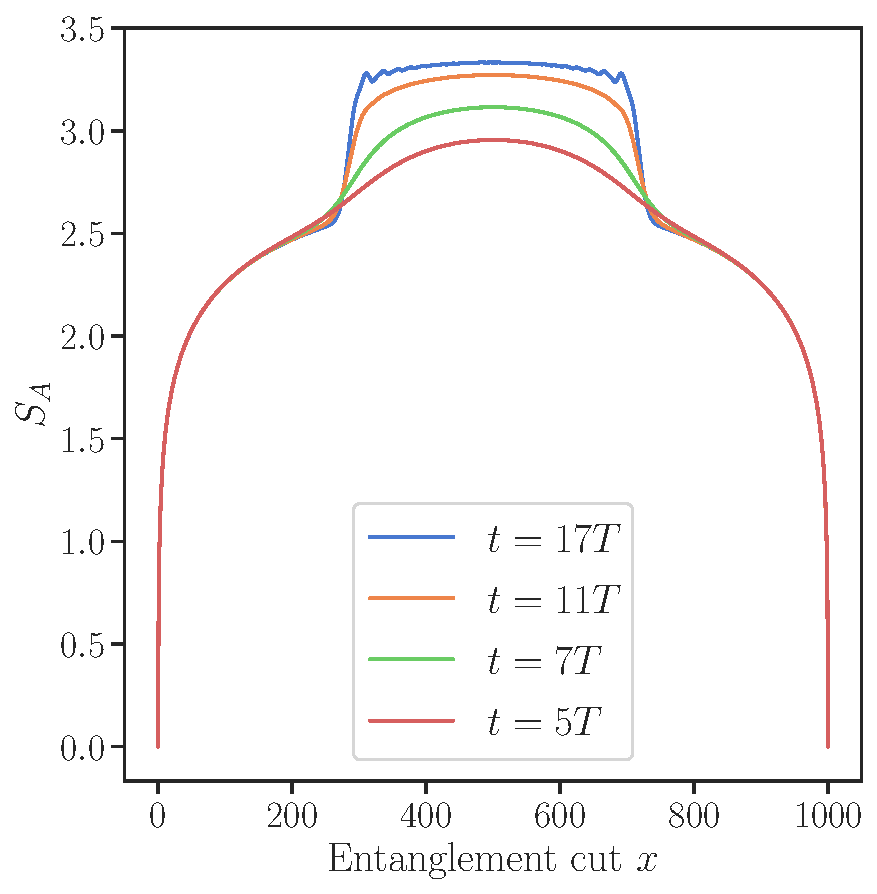
\includegraphics[width =\textwidth]{Entanglement_Entropy}
	\caption{}
	\label{EntanglementEvolution}
\end{subfigure}
\begin{subfigure}[t]{0.49\textwidth}
	\centering
	\includegraphics[width =\textwidth]{Entanglement_Entropy_relation}
	\caption{}
	\label{Entanglement_relation-energy}
\end{subfigure}
\caption{(a) Evolution of entanglement entropy as a function of the entanglement cut $x$ for the subsystem $A[0:x]$. The Floquet system parameters are $T_0 = 0.95L$ and $T_1=0.05L$ and we have periodic boundary conditions (b) The entanglement entropy and $\log(E(n))/6$ are plotted as a function of the number of cycles to verify the correspondence \ref{eq:correspondence_total_energy_EE}}
\end{figure}

%\section{The quasi-particle picture}
%To provide an understanding for the formation of the two energy peaks one can aim to try to describe the evolution with the help of quasi-particles. The velocity of the quasi-particles at the beginning of each cycle is given by the sine-square envelope:
%\begin{equation}
%	v(x_i) = 2\sin^2(\pi x_i/L)
%\end{equation}
%since the operator products $\hat{c}_i \hat{c}_{i+1}$ and its adjoint represent kinetic terms.




%\begin{figure}[h]
%	\centering
%	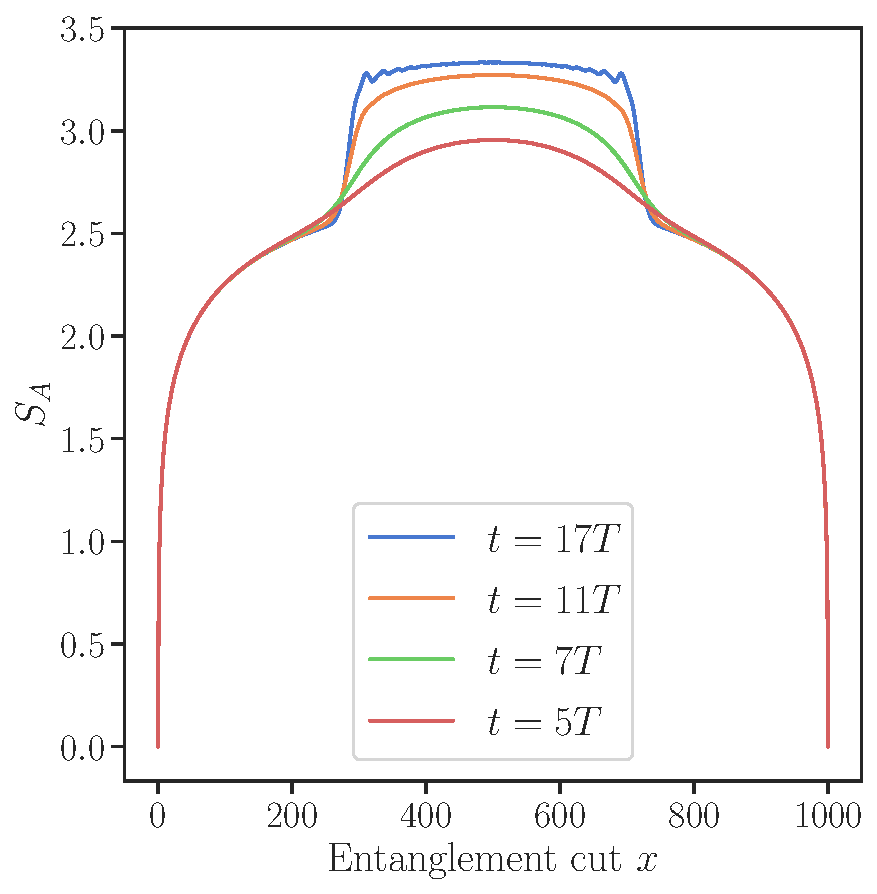
\includegraphics[width=0.8\textwidth]{Entanglement_Entropy}
%	\caption{Evolution of entanglement entropy as a function of the entanglement cut $x$ for the subsystem $A[0:x]$. The Floquet system parameters are $T_0 = 0.95L$ and $T_1=0.05L$ and we have periodic boundary conditions.}
%	\label{EntanglementEvolution}
%\end{figure}
%The observed entanglement pattern for the heating phase can be further understood by analyzing the emergence of quasi-particles and their behaviors as we change from the $\hat{H}_0$ to $\hat{H}_{\text{SSD}}$. Hamiltonian in any given Floquet driving cycle. 



\chapter{Floquet system in two dimensions}
In one-dimension, we have observed that the Floquet time evolution leads to a formation of two phases; heating and non-heating, depending on the driving parameters $T_0$ and $T_1$. We found that the numerical results on the lattice model in large parts were consistent with the predictions of Floquet conformal field theory. In this chapter, we wish to now analyze whether a similar phase structure can also be observed in a two-dimensional Floquet system on a lattice. It should be noted however that we will have to rely solely on numerics as there is no analytically solvable model available for a Floquet system in two dimensions.\\

 At $t=0$, we again, prepare the initial state $\ket{\psi(t=0)}$ to be the ground state of the periodic-tight-binding model\footnote{We employ periodic boundary conditions both in $x$ and $y$ directions}:
\begin{equation}
\begin{split}
	\hat{H}_0 =  \sum_{i = 1}^{L_x} \sum_{j=1}^{L_y}& \Big( -t_1 \left[ \hat{c}^\dagger(i, j) \hat{c}(i+1, j) + \hat{c}^\dagger(i+1, j)\hat{c}(i, j) \right] \\
	&-t_2 \left[\hat{c}^\dagger(i,j) \hat{c}(i,j+1) + \hat{c}^\dagger(i, j+1)\hat{c}(i,j) \right] \Big)
	\label{eq:Floquet_Hamiltonian0}
\end{split}
\end{equation}  
and then time evolve the ground state with the sine-squared deformed Hamiltonian for time $T_1$:
 \begin{equation}
 \begin{split}
		\hat{H}_\text{1} = \sum_{i=1}^{L_x-1} \sum_{j=1}^{L_y-1}\Big(&-t_1 \mathcal{F}\left(i+\frac{1}{2}, j\right) \left[ \hat{c}^\dagger(i,j)\hat{c}(i+1, j) + \hat{c}^\dagger(i+1,j) \hat{c}(i,j)\right]  \\
& -t_2 \mathcal{F}\left(i, j + \frac{1}{2}\right) \left[\hat{c}^\dagger(i, j) \hat{c}(i, j + 1) + \hat{c}^\dagger(i, j+1) \hat{c}(i,j) \right]\Big)
\label{eq:Floquet_Hamiltonian1}
\end{split}
\end{equation}
where $\mathcal{F}(x,y)$ corresponds to the function \ref{eq:sine_squared_deformation2d}. To complete a cycle, we then drive the state with $\hat{H}_0$ for a time $T_0$. To summarize, the time-dependent Hamiltonian is given by:
	\begin{equation}
	\hat{H}(t) = 
		\begin{dcases}
		\text{SSD-Hamiltonian } (\ref{eq:Floquet_Hamiltonian0}) \quad &0<t< T_1 \\
		\text{PBC-Hamiltonian } (\ref{eq:Floquet_Hamiltonian1}) \quad &T_1 < t < T_1 + T_0
		\end{dcases}
		\label{eq:Floquet_Hamiltonian2d}
	\end{equation}
where in both cases, we will for simplicity, set $t_1 = t_2$ = 1.
Since nothing about the protocol changes, the factorization of the Floquet operator \ref{eq:Floquet_operator_n_cycles} still holds. The only difference to the one-dimensional case is the extra degree of freedom resulting from a two-dimensional basis state being described by two indices rather than one, which leads to an ambiguity as to how the basis states are supposed to be ordered (i.e does the state $\ket{1,2}$ come before $\ket{2,1}$ or the other way around). For a square lattice, we have $L_x = L_y$ and therefore require $L^2$-basis states. In our numerical implementations we will stick to natural ordering, meaning we order the basis states $(i,j)$ as such:
\begin{itemize}
	\item Start at lattice location $(0,0)$, corresponding to the first element in the flattened vector and assign it index $k = 1$
	\item Increment $j$ to traverse the vertical $y$-direction.
	\item Once the end of the lattice has been reached, return to $j = 0$ and increment $i$ by one. This procedure is repeated such that the entire lattice has been indexed by $k$.
\end{itemize}
Once the basis-ordering has been decided upon, we proceed in a similar fashion as in 1D, by first obtaining the explicit matrix form for our Hamiltonians \ref{eq:Floquet_Hamiltonian0} and \ref{eq:Floquet_Hamiltonian1}. The shape of the resulting matrices are shown in the Fig. below:
\begin{figure}[h]
\centering
		\begin{subfigure}[b]{0.31\textwidth}
			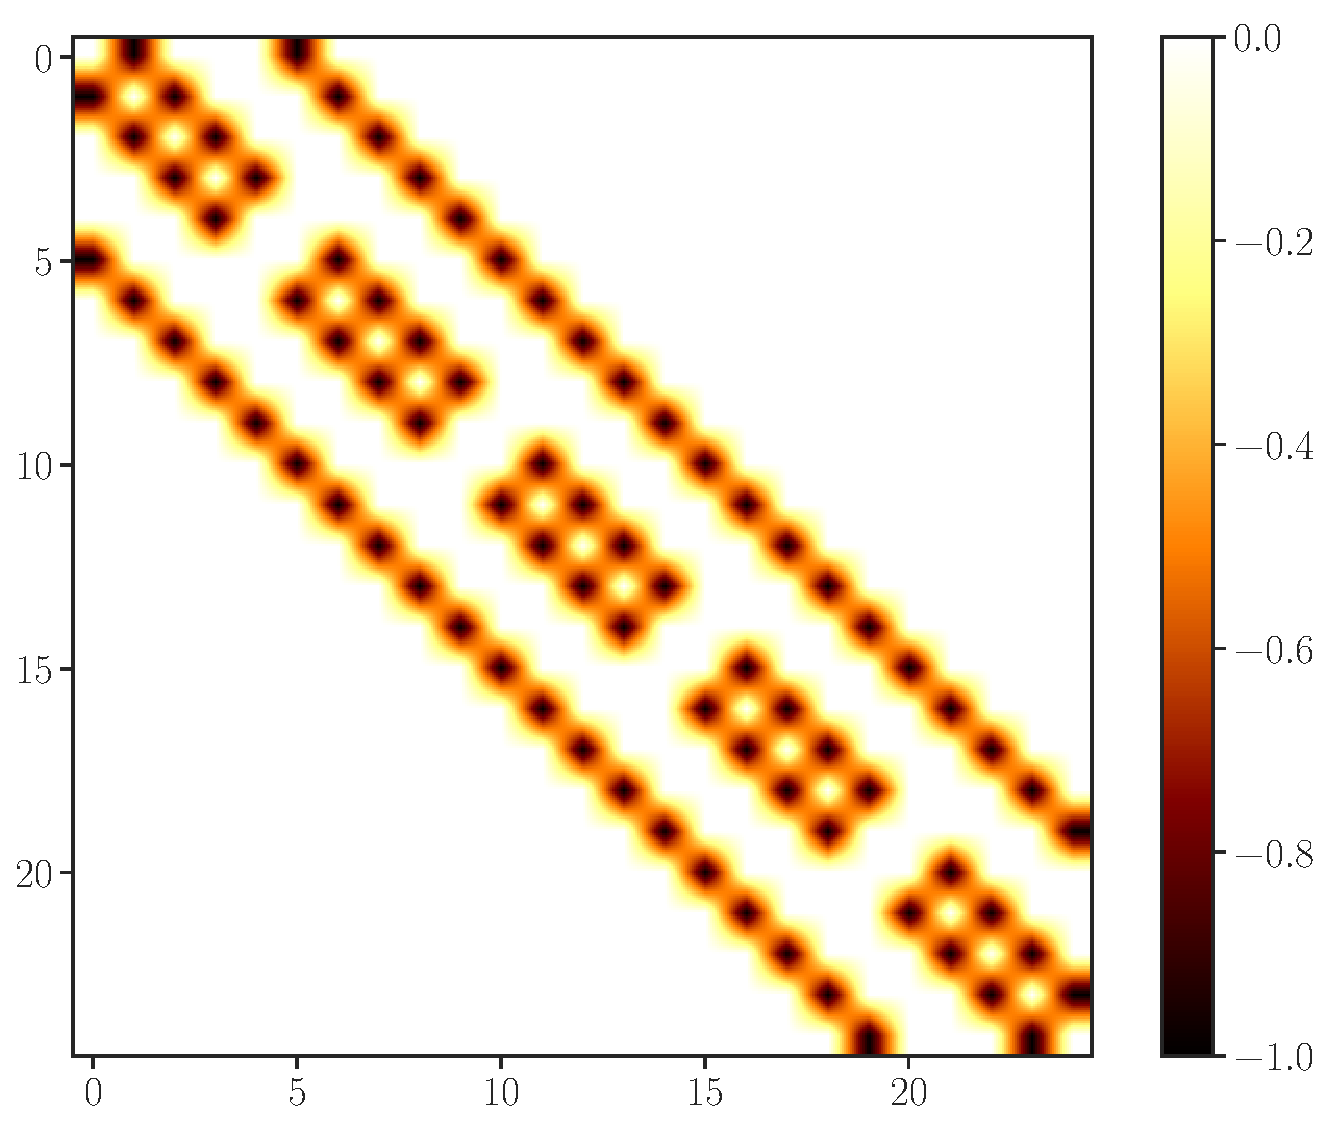
\includegraphics[width=\textwidth]{ColorMapMatrix_OBC_2D}
			\caption{}
		\end{subfigure}
		\begin{subfigure}[b]{0.31\textwidth}
			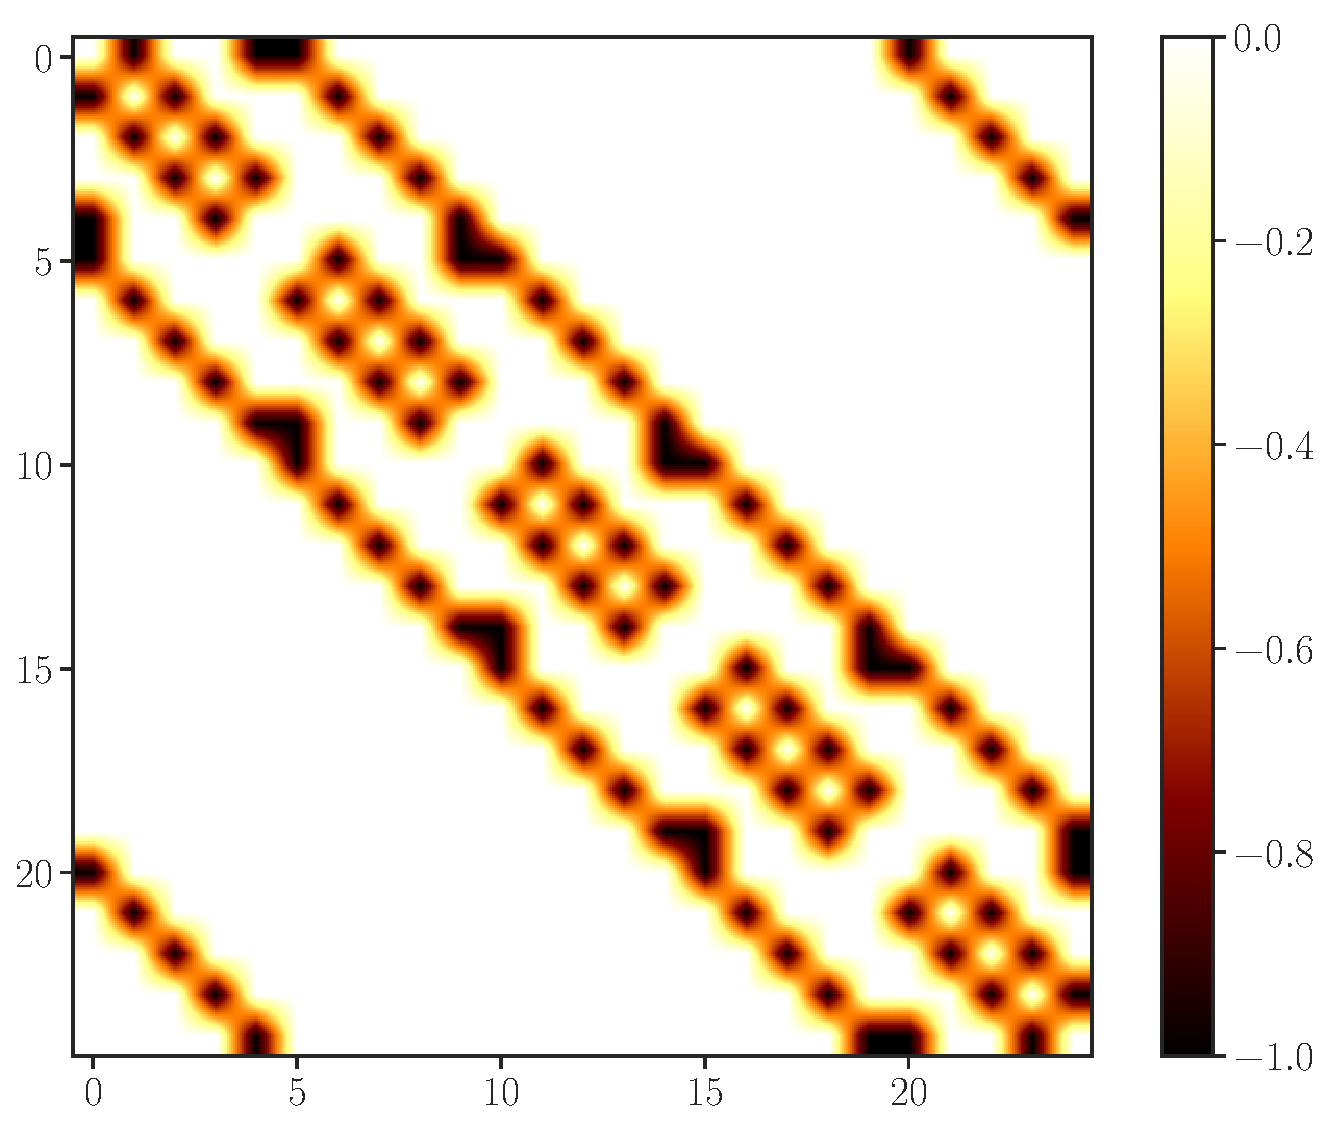
\includegraphics[width=\textwidth]{ColorMapMatrix_PBC_2D}
			\caption{}
		\end{subfigure}
		\begin{subfigure}[b]{0.31\textwidth}
			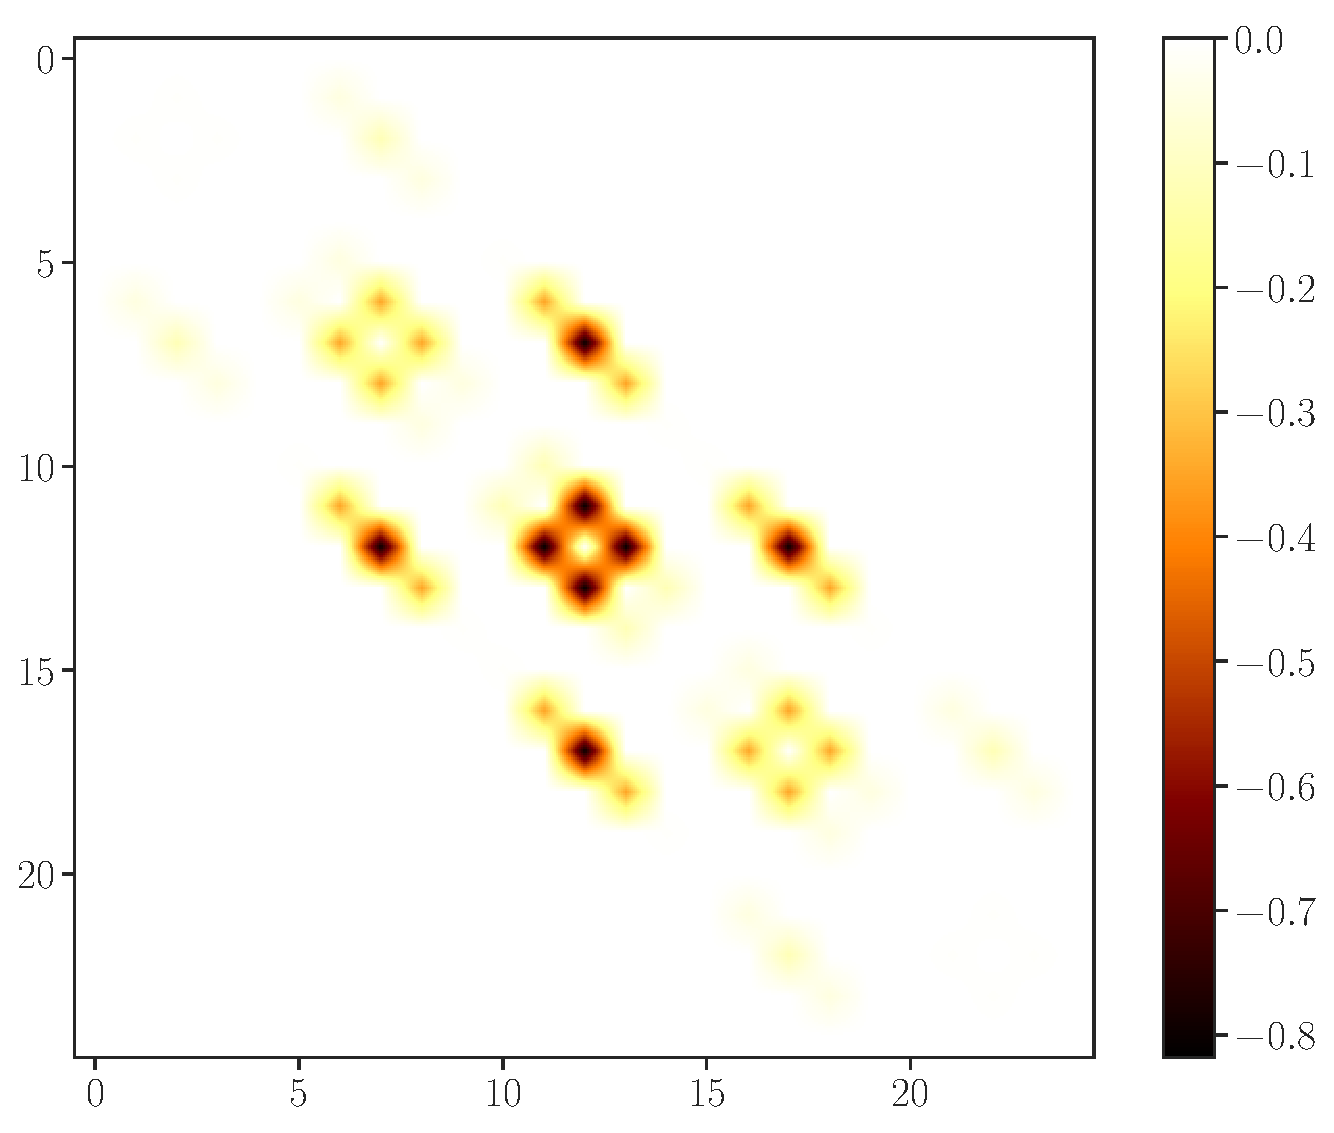
\includegraphics[width = \textwidth]{ColorMapMatrix_SSD_2D}	
			\caption{}
		\end{subfigure}
		\caption{Structure of the tight-binding Hamiltonian for $L_x = L_y = 5$ and (a) open-boundary conditions (b) periodic-boundary conditions (c) sine-squared deformed.}
\end{figure}
The procedure to obtain the correlation function after $n$-cycles for the two-dimensional case, follows analogously the procedure introduced in section \ref{sec:correlation_function_1d}. The only difference is the dimensions of the matrices and the number of occupied modes. The correlation function after $n$-cycles is still given by \ref{eq:correlation_matrix_Xueda}. 
\section{Total energy}
The total energy for the two-dimensional lattice in terms of the two-point correlation function is simply given by:
\begin{equation}
\begin{split}
E(n) =\expval*{\hat{H}_0} = \mel{\psi(nT)}{\hat{H}_0}{\psi(nT)} = \sum_{i=1}^{L-1}\sum_{j=1}^{L-1} & \Big(\mathcal{C}[(i,j),(i+1,j)] + \mathcal{C}[(i,j), (i, j+1)] \\
 &+ \mathcal{C}[(i+1,j),(i,j)] + \mathcal{C}[(i,j+1), (i,j)] \Big)
\end{split}
\end{equation}
Similarly, to the one-dimensional case, we wish to analyze the heating and non-heating phase structure. The results obtained for a square lattice with $L_x = L_y = 15$ sites after $5$-cycles, is shown in Fig. \ref{Phase-structure2d}. Due to the low resolution, we note, that the exact transition lines in the phase structure, namely in the ranges shortly after a period are hard to make out\footnote{This is suspected to be the case due to the small system size of only $L = 15$}. However a comparison with Fig. \ref{fig:Phase_Diagram_Total_Energy}, still allows for the conclusion that the phase-structure period in the two-dimensional case, is $1/4$-th that of the one-dimensional one.  Not surprisingly, we also observe, that due to the larger degrees of freedom and the larger Hilbert space, the total energy values are substantially larger than in the one-dimensional case. \\

\begin{figure}[h]
\centering
\begin{subfigure}[t]{0.49\textwidth}
	\centering
	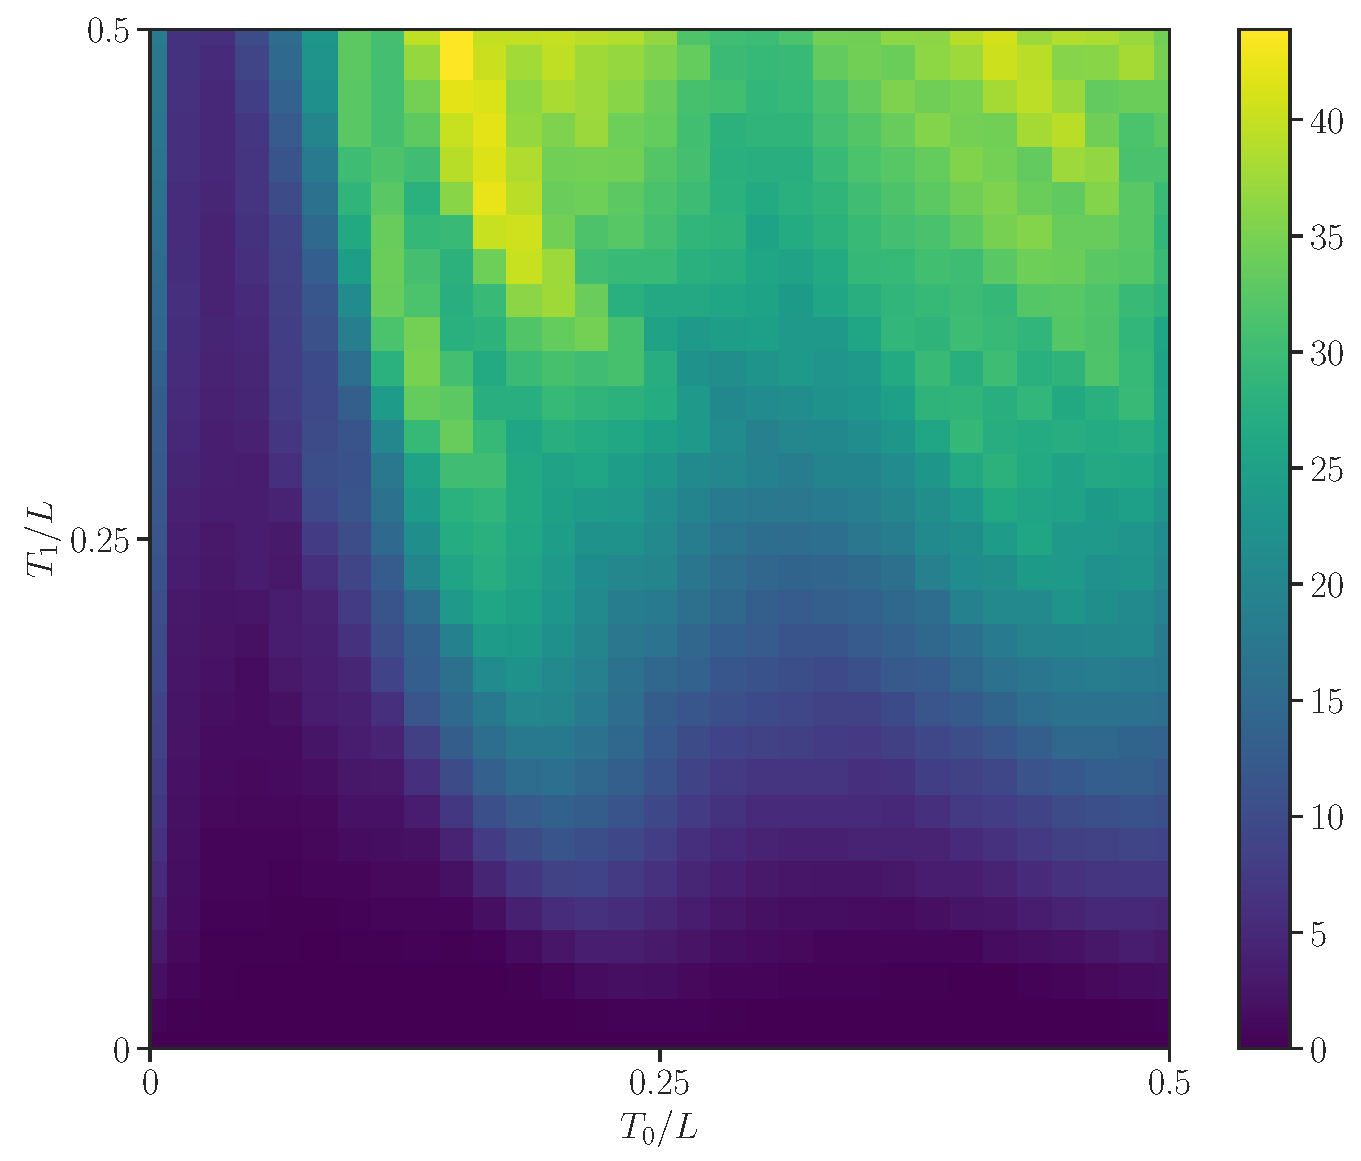
\includegraphics[width =\textwidth]{PhaseDiagram2D}
\end{subfigure}
\begin{subfigure}[t]{0.49\textwidth}
	\centering
	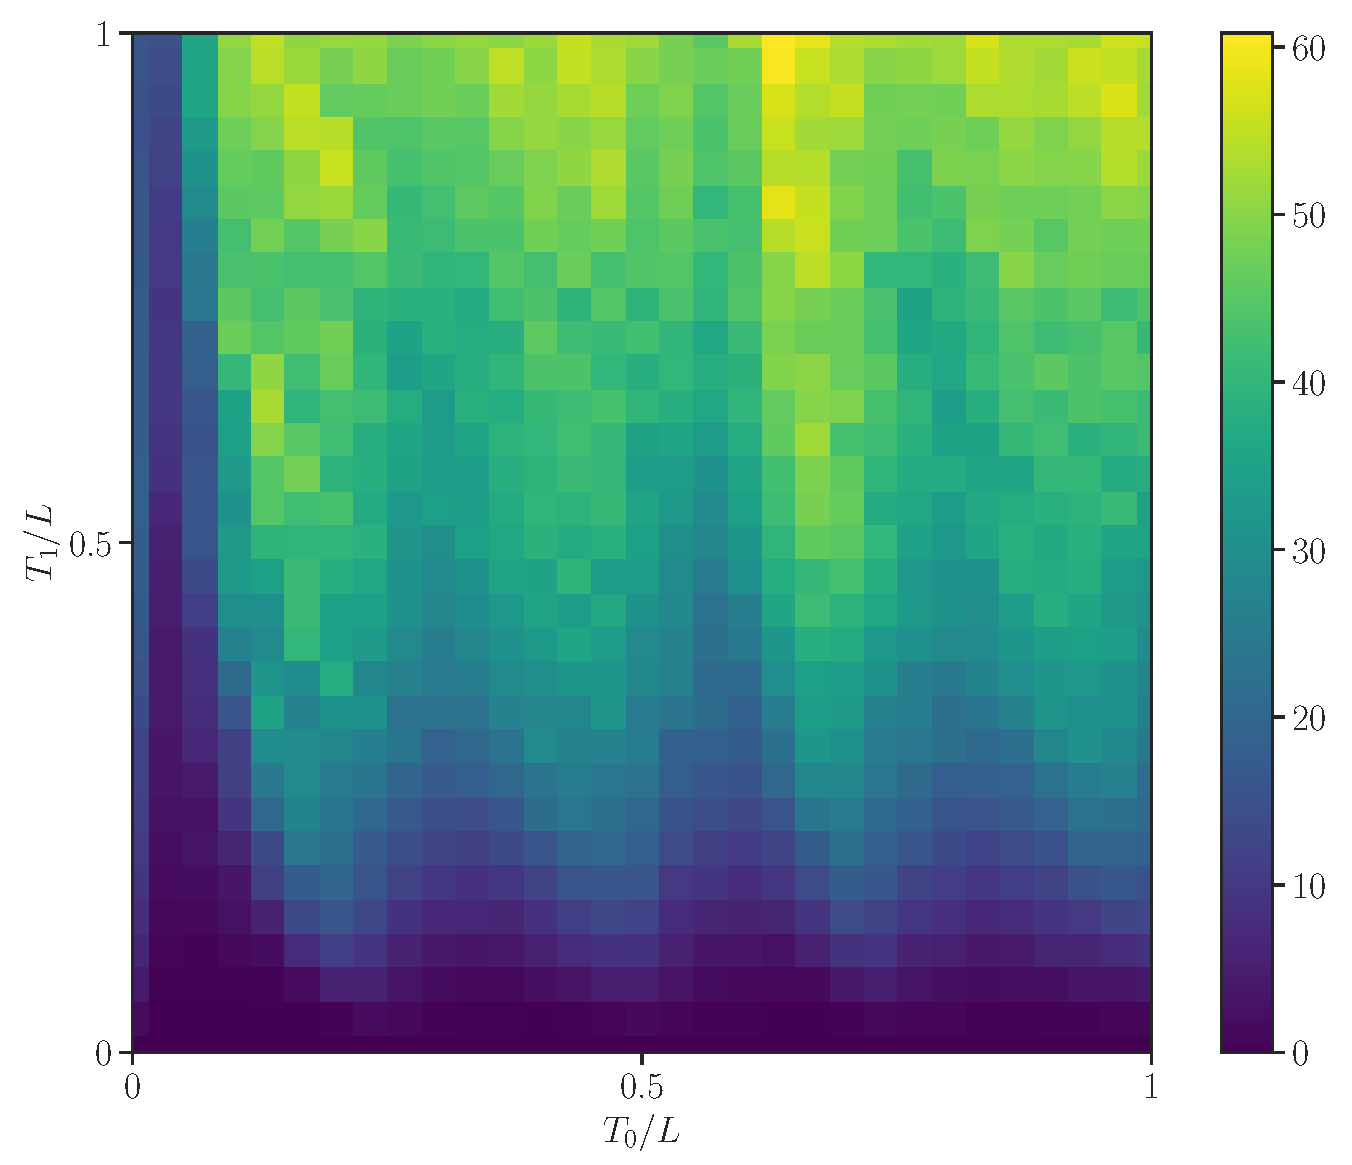
\includegraphics[width =\textwidth]{PhaseDiagram2D-2}
\end{subfigure}
\caption{Phase diagram for a 5-cycle driven two-dimensional square lattice with $L_x = L_y =15$ and periodic boundary conditions.}
\label{Phase-structure2d}
\end{figure}
In the next step, we wish to analyze the evolution of the total energy for the heating and non-heating phase. The results for two examples of a heating and non-heating phase are shown in Fig. \ref{fig:Total_energy_evolution}. The heating phase is similar to the one-dimensional case  where it shows a steep increase in total energy for the first few cycles until the energy saturates at around $E =140$ and oscillates slightly around that value. A similar behavior for other heating phases can be observed in Fig. \ref{Total_Energy_heating2d-multiple}.  In contrast to the one-dimensional case, we observe that the non-heating phase is not periodic anymore but rather stays constrained within an energy window between $E = 12.5$ and $E=17.5$, meaning that in the non-heating case, the system stays constrained in a very small sector of the total Hilbert space and never returns to its initial ground state. The reason for this is that, in one-dimension, the particles were restricted to moving left or right, meaning the probability that the trajectory of all quasiparticle at time $t$ returns them to their initial position, is much more likely than in the two-dimensional case due to the higher degrees of freedom.

\begin{figure}[h]
\centering
\begin{subfigure}[t]{0.49\textwidth}
	\centering
	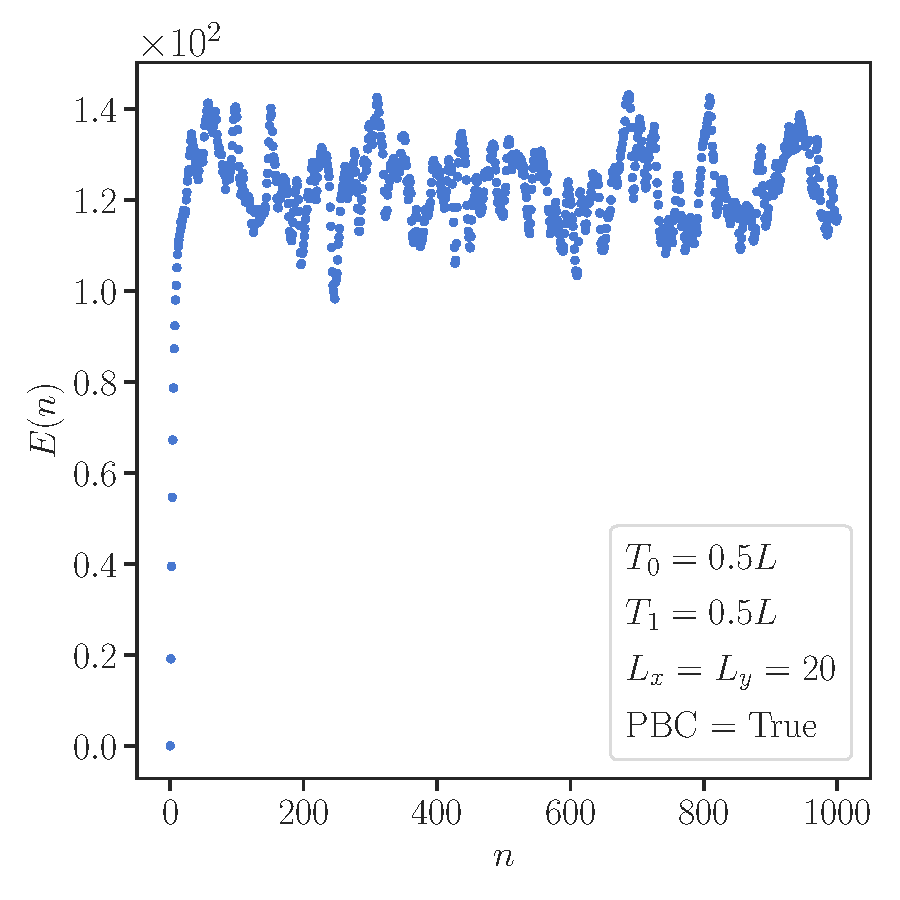
\includegraphics[width =\textwidth]{TotalEnergyHeating2d}
\end{subfigure}
\begin{subfigure}[t]{0.49\textwidth}
	\centering
	\includegraphics[width =\textwidth]{TotalEnergyNonHeating2d}
\end{subfigure}
\caption{Total energy evolution as a function of the cycles for a (left) heating phase and (right) non-heating phase}
\label{fig:Total_energy_evolution}
\end{figure}

In Fig. \ref{Evolution_total_energy_differentT1}, we can furthermore see that by increasing $T_1$, the system slowly transitions from a non-heating phase to a heating phase where an ever-growing energy bandwidth can be observed.
\begin{figure}[h]
\centering
\includegraphics[width = 0.85\textwidth]{TotalEnergyNonHeating2d_Multiple}
\caption{Evolution of total energy $E(n)$ for the two-dimensional Floquet System as a function of the number of cycles $n$ for different parameters of $T_1$. }
\label{Evolution_total_energy_differentT1}
\end{figure}



\section{Energy density}
Lastly, we will study the energy density of our Floquet system. This quantity can again be expressed in terms of the two-point correlation function: 
\begin{equation}
\begin{split}
	\mathcal{E}(i,j,n) =  & \mathcal{C}[(i,j),(i+1,j)] + \mathcal{C}[(i,j), (i, j+1)] \\
 &+ \mathcal{C}[(i+1,j),(i,j)] + \mathcal{C}[(i,j+1), (i,j)]
\end{split}
\end{equation}
In contrast to the one-dimensional case, however, in two-dimension a clear pattern characterizing the heating and non-heating cannot be found.  This becomes evident when looking at the results obtained in Fig. \ref{eq:Energy_density_heating2d} where no reoccurring pattern amongst all different highly-symmetric heating phases emerges. This means that even though there seems to be a tendency for energy to accumulate away from the centers of the system and more towards the boundary, no clear notion of heating and non-heating sectors can be determined. It should also be noted that the bandwidth of energy values, i.e the highest energy values and lowest energy value in the energy density spectrum, is more narrow in two- than in one-dimension, meaning the heating occurs in a more spatially uniform way compared to the case in one-dimension, where only the chiral and anti-chiral peaks absorb the heat at early times. \\

 For certain choices of parameters, however, the distinction between heating and non-heating sectors can still become quite pronounced.  Such an example is shown in Fig. \ref{fig:Energy_density2d-1}, where a clear circular heating sector can be found.

\begin{figure}[h]
\begin{subfigure}{.5\textwidth}
  \centering
  \includegraphics[width=\linewidth]{heatmapED_2D-heating1.pdf}
  \caption{}
\end{subfigure}
\begin{subfigure}{.5\textwidth}
  \centering
  \includegraphics[width=\linewidth]{heatmapED_2D-heating2.pdf}  
  \caption{}
\end{subfigure}
\begin{subfigure}{.5\textwidth}
  \centering
  \includegraphics[width=\linewidth]{heatmapED_2D-heating3.pdf}
  \caption{}
\end{subfigure}
\begin{subfigure}{.5\textwidth}
  \centering
  \includegraphics[width=\linewidth]{heatmapED_2D-heating4.pdf}  
  \caption{}
\end{subfigure}
\caption{Energy density for 10 cycles and a square Lattice with $L_x = L_y = 50$ for the time parameters (a) $T_0 = T_1 = 0.5L$ (b) $T_0 = 0.5L$, $T_1 = 0.9L$ (c) $T_0 = 0.2L, T_1 = 0.5L$ (d) $T_0 = 0.2L, T_1 = 0.2L$}
\label{eq:Energy_density_heating2d}
\end{figure}

\begin{figure}[h]
\centering
\includegraphics[width=0.8\textwidth]{Energydensity2d_nearest.pdf}	
\caption{Heating phase for the 2D Floquet System after 10 cycles for a system of $L = 50$ Lattice Sites. The parameters here are $T_0 = -0.5L$ and $T_1 = 0.5L$.}
\label{fig:Energy_density2d-1}
\end{figure}
%\begin{figure}[h]
%\centering
%\begin{subfigure}[t]{0.49\textwidth}
%	\centering
%	\includegraphics[width =\textwidth]{Energydensity2d_nearest.pdf}
%\end{subfigure}
%\begin{subfigure}[t]{0.49\textwidth}
%	\centering
%	\includegraphics[width =\textwidth]{Energy_Density2D_nearest2.pdf}
%\end{subfigure}
%\caption{(left) (right)}
%\end{figure}


%\begin{figure}[h]
%\centering
%\begin{subfigure}[t]{0.49\textwidth}
%	\centering
%	\includegraphics[width =\textwidth]{TotalEnergyHeating2d}
%\end{subfigure}
%\begin{subfigure}[t]{0.49\textwidth}
%	\centering
%	\includegraphics[width =\textwidth]{TotalEnergyNonHeating2d}
%\end{subfigure}
%\caption{(left) Total Energy Evolution as a function of the cycles for a heating phase (right)}
%\end{figure}



\chapter{Conclusion}
The bulk of this thesis included verifying the analytical predictions made by Floquet CFT by simulating the dynamics of the Floquet system numerically on a lattice. Even though no solvable framework for this case currently exists, we then conducted a study analyzing whether similar predictions for the two-dimensional system can be made. \\

In one-dimension an emergence of a heating and non-heating phase was observed. In the non-heating phase, the total energy and entanglement entropy were found to periodically oscillate as a function of the number of cycles $n$. The characteristic feature of the heating phase was the formation of two energy absorbing accumulation points, the chiral and anti-chiral peak, which were found to share the entirety of the systems entanglement entropy. The total energy (in the early-time driving regime) was additionally found to be exponentially increasing. All of the above the obtained results seemed to match the predictions made by the Floquet CFT. The only significant departure from the analytical predictions is the expected relation between entanglement entropy and total energy of the system.\\

In the two-dimensional square lattice system, a similar phase structure as in one-dimension was observed. A notable change, however is the decrease of the phase-structure periodicity from 1 to $1/4$-th. We also observed that the periodicity of the total energy for the non-heating phase was broken. Instead, the phase gets stuck in a narrow energy window and never returns to its initial ground state energy. \\


We also found that the clear notion of chiral and anti-chiral energy accumulation points in one-dimension, have no corresponding counterpart in two-dimensions. It turns out that the shape and location of the heating sectors greatly vary for different heating phases. This can be reasoned by arguing that a two-dimensional system has more degrees of freedom, leading to more varied trajectories of the quasiparticles. The probability of quasiparticles accumulating at the same lattice site is therefore a lot less likely than in one-dimension.\\

Further investigations of the two-dimensional system could include analyzing the evolution of the entanglement entropy. Due to the natural ordering of the basis states, identifying the correct corresponding state sub-sectors for the bipartition of the total system, may pose complications in its implementation. The question then naturally arises, whether entanglement entropy and total energy share a correspondence  similar to the one obtained in one-dimension\footnote{We do not refer to the Floquet CFT energy-entanglement prediction here}. Finally, the resulting dynamics of different initial states, such as a thermal one, could be studied.

\printbibliography[heading=bibintoc,title={Bibliography}]
\newpage


\begin{appendices}
\appendix
\appendixpage
\addappheadtotoc
\chapter{Additional Information}
\section{Thermal initial state}
Instead of considering the initial state of our Floquet system to be the pure ground state of $\hat{H}_0$ at temperature $T=0$ with Fermi-Dirac distribution \ref{Fermi-Dirac-DistributionT=0}, we can also consider a thermal state at thermal equilibrium. To study the expectation value at finite temperatures, we resort to the density matrix formalism. In the canonical ensemble (fixed $N$, $V$ and $T$), the probabilities of the energy eigenstates $\ket{\psi_i}$ are proportional to the Boltzmann factor $p_i \propto \exp(-\beta E_i)$, where $k_BT = 1/\beta$. As such, the density matrix reads
\begin{equation}
	\rho = \sum_{i} e^{-\beta E_i} \ket{\psi_i} \bra{\psi_i} = e^{-\beta \hat{H}_0}
\end{equation}
The expectation value of an observable $\mathcal{O}$ is then given by:
\begin{equation}
	\expval{\mathcal{O}} = \frac{\text{Tr}[\mathcal{O}\rho]}{\text{Tr}(\rho)} = \frac{1}{Z} \sum_i e^{-\beta E_i} \mel{\psi_i}{\mathcal{O}}{\psi_i}
\end{equation}
where $Z$ denotes the canonical partition function $Z = \sum_i e^{-\beta E_i}$. It can be shown that the two-point correlation function $\mathcal{C}_{ij} = \expval{\hat{c}_i \hat{c}_j}$ for the initial state simply has to be modified as such:
\begin{align}
		\mathcal{C}_{ij} &= \frac{1}{\text{Tr}(e^{-\beta \hat{H}_0})} \sum_{\{n_k\}}\mel{\{n_k\}}{\hat{c}_i^\dagger \hat{c}_j}{\{n_k\}} e^{-\beta \sum_k n_k \epsilon_k} \\
		&= \frac{1}{\text{Tr}(e^{-\beta \hat{H}_0})} \sum_{k} U_{ki}^* U_{kj} \sum_{\{n_k\}} \mel{\{n_k\}}{\hat{c}_k^\dagger \hat{c}_k}{\{n_k\}}e^{-\beta \sum_k n_k \epsilon_k} \\
		& = \sum_k U_{ki}^* U_{kj} \expval{n_k}
\end{align}
where we used the unitary transformation $U$ which diagonalizes $\hat{H}_0$ and \ref{eq:inverse_transformation_operators2nd}. To obtain the correlation function at later times, the same procedure can be applied. It should be noted that in the CFT Calculations, the phase heating/non-heating phase structure will remain even if the system is prepared in a thermal state \cite{Fan}.


\section{Witt Algebra}
To find the algebra of the generators we consider the infinitesimal conformal transformation
\begin{equation}
\begin{split}
	z &\rightarrow \tilde{z} = z + \epsilon(z), \quad \epsilon(z) = \sum_{n = -\infty}^\infty c_n (-z^{n+1}) \\
	\bar{z} &\rightarrow \bar{z} + \bar{\epsilon}(\bar{z}) = \bar{z}, \quad \bar{\epsilon}(\bar{z}) = \sum_{n = -\infty}^\infty \bar{c}_n (- \bar{z}^{n+1})
\end{split}
\end{equation}
where the infinitesimal parameters $\epsilon_n$ and $\bar{\epsilon}_n$ are constant. The differential operators that generate the infinitesimal transformations are
\begin{equation}
	L_n = -z^{n+1} \partial_z, \quad \bar{L}_n = - \bar{z}^{n+1} \partial_{\bar{z}}
\end{equation}
These operators satisfy the following commutation relation
\begin{equation}
	\comm{L_m}{L_n} = (m-n)L_{m+n}, \quad \comm{\bar{L}_m}{\bar{L}_n} = (m - n) \bar{L}_{m + n}, \quad \comm{L_m}{\bar{L}_n} = 0
\end{equation}
These two algebras are independent of each since they $L_n$'s and $\bar{L}_m$'s commute with each other meaning that the (local) conformal algebra is simply the direct sum of the two isomorphic algebras $\mathcal{A}. \oplus \bar{\mathcal{A}}$. Since these two are independent we therefore say $z$ and $\bar{z}$ are independent since the action of the conformal group in two dimensions factorizes into independent actions on $z$ and $\bar{z}$ and we are effectively considering $\mathbb{C}^2$ and $\mathbb{C}$. The generator for an arbitrary conformal transformation is thus
\begin{equation}
	\sum_n c_n L_n + \bar{c}_n \bar{L}_n
\end{equation}
and generates conformal transformations of functions $f(z, \bar{z})$ \cite{Schellekens,Francesco}

%\subsubsection{Global subgroup}
% It should be noted that the algebra of infinitesimal conformal transformation in an Euclidean two-dimensional space is infinite-dimensional. However we run into a problem, as the Witt algebra generated by the set $\{L_n\}$ is not well defined everywhere on the Euclidean plane $\mathbb{R}^2 \simeq \mathbb{C}$. It is clear that it is necessary not to work on $\mathbb{C}$ but rather on the Riemann sphere $S^2 \simeq \mathbb{C} \cup \infty$ as it is the conformal compactification of $\mathbb{R}^2$. We find that for the generators to be non-singular at the two points $z = 0$ and $z=\infty$ certain restrictions on the values of $n$ have to be imposed. We find that only the the finite subalgebra consisting of the operators $\{L_{-1}, L_0, L_{+1} \}$ are globally well defined and generate the so-called global conformal transformation on the Riemann sphere $S^2 = \mathbb{C} \cup \infty$. We identify $L_{-1} = - \partial_z$ and $\bar{L}_{-1}$ as the generators of translations,
%\begin{center}
%\begin{tabular}{ccc}
%Generator & Local Transformation & Global Transformation \\
%\hline
%	$-\epsilon L_{-1}$ & $z \rightarrow z + \epsilon$ & $z \rightarrow z + \alpha $\\
%	$-\epsilon L_0$ & $z \rightarrow z + \epsilon z$ & $z \rightarrow \lambda z$ \\
%	$-\epsilon L_1 $& $z \rightarrow z + \epsilon z^2  $& $z \rightarrow z/(1-\beta z)$ \\
%\end{tabular}
%\end{center}
%
%What will become evident, is that the conformal group on the Riemann sphere is simply the Möbius group SL$(2, \mathbb{C})/ \mathbb{Z}^2$ as combining the above transformation in the table we get
%\begin{equation}
%	z \rightarrow \frac{az + b}{cz + d}, \; \bar{z} \rightarrow \frac{\bar{a} \bar{z} + \bar{b}}{\bar{c} \bar{z} + \bar{d}} \qq{with} ad-bc = 1
%\end{equation}


\chapter{Additional Plots}
\begin{figure}
\centering
\includegraphics[width = 0.75\textwidth]{TotalEnergyHeating2d_Multiple}
\caption{Evolution of the total energy for different parameters $T_1/L$ of a heating phase.}
\label{Total_Energy_heating2d-multiple}
\end{figure}


\begin{figure}
\centering
\includegraphics[width = 0.75\textwidth]{Energy_Density_late-time-regime}
\caption{The energy density in the late-time regime for a lattice of $L=1000$ sites and parameters $T_0/L = 0.95$ and $T_1/L = 0.05$.}
\label{fig:Energy_density-late-regime}
\end{figure}



\begin{figure}
\begin{subfigure}{.5\textwidth}
  \centering
  \includegraphics[width=\linewidth]{eigenstate_profile2D_H0-2}
  \caption{}
\end{subfigure}
\begin{subfigure}{.5\textwidth}
  \centering
  \includegraphics[width=\linewidth]{eigenstate_profile2D_H0.pdf}  
  \caption{}
\end{subfigure}

\begin{subfigure}{.5\textwidth}
  \centering
  \includegraphics[width=\linewidth]{eigenstate_profile2D.pdf}
  \caption{}
\end{subfigure}
\begin{subfigure}{.5\textwidth}
  \centering
  \includegraphics[width=\linewidth]{eigenstate_profile2D-1.pdf}  
  \caption{}
\end{subfigure}
\caption{Spatial probability distribution for the eigenfunctions (a) $\abs{\varphi_2(x,y)}^2$ and (b) $\abs{\varphi_{12}(x,y)}^2$ fof the PBC tight-binding model and (c) $\abs{\varphi_{501}(x,y)}^2$ and (d) $\abs{\varphi_{1600}(x,y)}^2$ for the SSD deformed model on a square lattice of size $L_x = L_y = 50$. The index in the subscript denotes the energy level $l$.}
\end{figure}

\begin{figure}
\centering
		\begin{subfigure}[b]{0.45\textwidth}
			\includegraphics[width=\textwidth]{DensityprofileOBC}
			\caption{}
		\end{subfigure}
		\begin{subfigure}[b]{0.45\textwidth}
			\includegraphics[width=\textwidth]{DensityprofileSSD}
			\caption{}
		\end{subfigure}
		\caption{Density profile $\expval{n(x,y)} = \sum_{i (E_i < 0)} \abs{\varphi_{i}(x,y)}^2$ of the groundstate for (a) open boundary conditions, (b) sine squared deformed. As is the case in one-dimension, the sine-squared deformation shows translational invariance in the bulk of the system while still maintaining some boundary effects on the edges of the system.}
\end{figure}
\end{appendices}






\end{document}